%%
%% This is file `thesis.tex',
%% generated with the docstrip utility.
%%
%% The original source files were:
%%
%% nudtpaper.dtx  (with options: `thesis')
%%
%% This is a generated file.
%%
%% Copyright (C) 2018 by TomHeaven <hanlin_tan@nudt.edu.cn>
%%
%% This file may be distributed and/or modified under the
%% conditions of the LaTeX Project Public License, either version 1.3a
%% of this license or (at your option) any later version.
%% The latest version of this license is in:
%%
%% http://www.latex-project.org/lppl.txt
%%
%% and version 1.3a or later is part of all distributions of LaTeX
%% version 2004/10/01 or later.
%%
%% To produce the documentation run the original source files ending with `.dtx'
%% through LaTeX.
%%
%% Thanks LiuBenYuan <liubenyuan@gmail.com> for maintainence.
%% Thanks Xue Ruini <xueruini@gmail.com> for the thuthesis class!
%% Thanks sofoot for the original NUDT paper class!
%%
%1. 规范硕士导言
% \documentclass[master,ttf]{nudtpaper}
%2. 规范博士导言
% \documentclass[doctor,twoside,ttf]{nudtpaper}
%3. 如果使用是Vista
% \documentclass[master,ttf,vista]{nudtpaper}
%4. 建议使用OTF字体获得较好的页面显示效果
%   OTF字体从网上获得，各个系统名称统一，不用加vista选项
%   如果你下载的是最新的(1201)OTF英文字体，建议修改nudtpaper.cls，使用
%   Times New Roman PS Std
% \documentclass[doctor,twoside,otf]{nudtpaper}
%   另外，新版的论文模板提供了方正字体选项FZ，效果也不错哦
% \documentclass[doctor,twoside,fz]{nudtpaper}
%5. 如果想生成盲评，传递anon即可，仍需修改个人成果部分
% \documentclass[master,otf,anon]{nudtpaper}
%
\documentclass[master,ttf,anon]{nudtpaper}
%\usepackage{lmodern} % 这个包导致英文字体与Word的渲染效果不一致，故去掉
\usepackage{mynudt}
\usepackage{multirow,array}
\usepackage{tikz,amsmath}
\usetikzlibrary{decorations.pathreplacing}

\classification{TP181}
\serialno{1605xxxx}
\confidentiality{公开}
\UDC{004.8}
\title{基于KAN的因果结构与函数联合发现方法研究}
\displaytitle{基于 KAN 的因果结构与函数联合发现方法研究}
\author{马一鸣}
\zhdate{\zhtoday}
\entitle{Research on KAN-based Joint Discovery Method for Causal Structure and Function}
\enauthor{Yiming Ma}
\endate{\entoday}
\subject{管理科学与工程}
\ensubject{Management Science and Engineering}
\researchfield{信息管理和信息系统}
\supervisor{黄宏斌\quad{}研究员}
\cosupervisor{}  % 协助指导教师，没有就空着
\ensupervisor{Prof. Hongbin Huang}
\encosupervisor{} % 协助指导教师英文，没有就空着
\papertype{工学}
\enpapertype{Engineering}
% 加入makenomenclature命令可用nomencl制作符号列表。

\begin{document}
	\graphicspath{{figures/}}
	% 制作封面，生成目录，插入摘要，插入符号列表 \\
	% 默认符号列表使用denotation.tex，如果要使用nomencl \\
	% 需要注释掉denotation，并取消下面两个命令的注释。 \\
	% cleardoublepage% \\
	% printnomenclature% \\
	\maketitle
	\frontmatter
	\tableofcontents
	\listoftables
	\listoffigures

	\midmatter
	\begin{cabstract}
当前人工智能系统多依赖数据中的统计相关性，缺乏可解释性与鲁棒性。因果发现旨在从观测数据中揭示变量间内在作用机制，是推动人工智能从“关联驱动”向“因果驱动”演进的关键。然而，现有因果发现方法多聚焦于有向无环图（DAG）结构学习，忽视了对结构因果模型中因果函数的刻画。传统深度学习求解器基于通用逼近定理设计，其稠密连接与黑箱特性使得学到的因果机制缺乏可解释性。此外，现有方法应对真实场景数据，并且模型难以支持精确的干预决策与反事实推理。鉴于此，本文引入柯尔莫哥洛夫 - 阿诺德网络（KAN），利用其符号化潜力与函数分解特性，研究基于 KAN 的因果结构与函数联合发现方法。

首先，提出基于 KAN 的连续优化因果发现算法（DAG-KAN）。针对现有方法重结构轻机制的局限，该算法构建轻量级单层 KAN 架构，实现因果结构与函数映射的端到端联合学习。基于 Kolmogorov-Arnold 表示定理，利用可学习 B 样条基函数显式拟合变量间非线性因果机制。设计适配 KAN 结构的节点独立性矩阵，通过边稀疏性约束学习因果邻接矩阵，并引入 L1正则化策略作用于样条系数，实现因果边的自动剪枝。在连续优化框架下加入无环性约束，确保学习到有向无环图。实验表明，该方法在加性模型数据上的结构学习精度优于主流方法，在高维复杂场景下结构汉明距离平均降低 22.6\%，且函数拟合均方误差达到 $10^{-3}$ 精度。

其次，提出基于 KAN 的知识融合因果发现算法（Causal-KAN）。针对真实场景普遍存在的非参数或半参数数据，设计知识嵌入层与局部连接激活层架构。通过在输入层引入因果掩码机制，将部分已知因果父节点关系硬编码为网络约束，在保障因果忠实性的同时具有深层网络函数逼近能力。这种结构化先验有效缩小了模型搜索空间，避免非因果变量的干扰。实验表明，该方法通过嵌入因果知识可有效防止过拟合，且学习到的因果函数具有可解释性，对节点规模和噪声水平敏感度低，鲁棒性较好。

本文提出的 DAG-KAN 与 Causal-KAN 方法，将因果发现研究从因果存在性判断推进至因果作用机制解析，构建了兼具可解释性与实用鲁棒性的因果函数学习方法。该方法能够显式表达变量间的作用机制，为精准医疗、政策干预等需要理解干预效果的领域提供了可操作的因果知识。
\end{cabstract}
\ckeywords{因果发现；Kolmogorov-Arnold 网络；因果函数；知识融合}

\begin{eabstract}
Current artificial intelligence systems largely rely on statistical correlations in data, lacking interpretability and robustness. Causal discovery aims to uncover the intrinsic mechanisms underlying the relationships between variables in observational data, and is key to driving the evolution of artificial intelligence from a “correlation-driven” to a “causal-driven” paradigm. However, existing causal discovery methods primarily focus on learning directed acyclic graph (DAG) structures, neglecting the characterization of causal functions within structural causal models. Traditional deep learning solvers are designed based on general approximation theorems; their dense connections and black-box nature result in learned causal mechanisms that lack interpretability. Furthermore, existing methods struggle with real-world data, and the models often fail to support precise intervention decisions and counterfactual reasoning. In light of this, this paper introduces the Kolmogorov–Arnold Network (KAN) and leverages its symbolic potential and function decomposition capabilities to investigate a KAN-based method for the joint discovery of causal structures and functions.

First, we propose a continuous optimization-based causal discovery algorithm (DAG-KAN) based on KAN. To address the limitation of existing methods that prioritize structure over mechanism, this algorithm constructs a lightweight single-layer KAN architecture to achieve end-to-end joint learning of causal structure and function mapping. Based on the Kolmogorov-Arnold representation theorem, we use learnable B-spline basis functions to explicitly fit nonlinear causal mechanisms between variables. We design a node independence matrix tailored to the KAN structure, learn the causal adjacency matrix under edge sparsity constraints, and introduce an L1 regularization strategy applied to spline coefficients to achieve automatic pruning of causal edges. By incorporating acyclicity constraints within the continuous optimization framework, we ensure the learned graph is a directed acyclic graph (DAG). Experiments demonstrate that this method achieves higher structural learning accuracy than mainstream methods on additive model data, reduces the average structural Hamming distance by 22.6\% in high-dimensional complex scenarios, and attains a mean squared error of $10^{-3}$ in function fitting.

Second, we propose a knowledge-fusion causal discovery algorithm based on KAN (Causal-KAN). To address the prevalence of non-parametric or semi-parametric data in real-world scenarios, we design an architecture comprising a knowledge embedding layer and a locally connected activation layer. By introducing a causal masking mechanism at the input layer, we hard-code known causal parent-child relationships as network constraints, thereby ensuring causal fidelity while maintaining the function approximation capabilities of deep neural networks. This structured prior effectively reduces the model search space and avoids interference from non-causal variables. Experiments demonstrate that this method effectively prevents overfitting by embedding causal knowledge, and the learned causal functions are interpretable, exhibit low sensitivity to node scale and noise levels, and demonstrate good robustness.

The DAG-KAN and Causal-KAN methods proposed in this paper advance causal discovery research from determining the existence of causality to analyzing causal mechanisms, establishing a causal function learning method that combines interpretability with practical robustness. This method can explicitly express the mechanisms of action between variables, providing actionable causal knowledge for fields such as precision medicine and policy intervention that require an understanding of intervention effects.

\end{eabstract}
\ekeywords{Causal Discovery; Kolmogorov-Arnold Networks; Causal Function; Knowledge Fusion}


	\chapter*{符号使用说明}
% 可以根据需要在chapter后加星星/去掉星星

\begin{denotation}
	
	% 核心因果建模符号
	\item[$V$]           变量集合
	\item[$X_{i}$]       单个观测变量
	\item[$PA_{i}$]      变量$X_{i}$的父节点集合
	\item[$G$]           因果结构对应的有向无环图
	\item[$\mathcal{E}$] 因果图中的边集合
	\item[$W$]           因果邻接矩阵
	\item[$f_{i}$]       变量$X_{i}$的因果函数
	\item[$U_{i}$]       变量$X_{i}$的外生噪声项
	\item[SCM]           结构因果模型
	\item[SEM]           结构方程模型
	\item[FCM]           函数因果模型
	
	% KAN相关符号
	\item[KAN]           柯尔莫哥洛夫-阿诺德网络
	\item[$\phi_{j,i}$]  KAN中输入$X_{i}$到输出$X_{j}$的单变量激活函数
	\item[$B_{q}(x)$]    B样条基函数
	\item[$C_{j,i,q}$]   KAN的可学习系数）
	\item[$g$]           B样条基函数的网格分辨率
	\item[$k$]           B样条基函数的阶数
	
	% 算法与优化符号
	\item[DAG-KAN]       基于KAN的连续优化因果发现算法
	\item[Causal-KAN]    基于KAN的知识融合因果发现算法
	\item[$\lambda$]     正则化系数
	\item[$\ell_{1}$]    L1正则化
	\item[$\mathcal{L}$] 模型拟合损失函数
	\item[$h(W)$]        无环性约束函数
	\item[$\nabla$]      梯度算子
	\item[$\eta$]        优化器学习率
	
	% 评估指标符号
	\item[SHD]           结构汉明距离
	\item[TPR]           真正例率
	\item[FPR]           假正例率
	\item[MSE]           均方误差
	\item[$R^{2}$]       决定系数
	\item[$\rho$]        皮尔逊相关系数
	
	% 数据集与实验符号
	\item[ER模型]        埃尔德什-雷尼随机图模型
	\item[SF模型]        无标度随机图模型
	\item[$d$]           变量维度
	\item[$n$]           样本数量
	\item[$\sigma$]      噪声水平
	
	% 其他常用符号
	\item[$\partial_{k}f_{j}$] 函数$f_{j}$对变量$X_{k}$的偏导数
	\item[$\|\cdot\|_{F}$] 弗罗贝尼乌斯范数
	\item[$tr(\cdot)$]   矩阵的迹
	
\end{denotation}


	%书写正文，可以根据需要增添章节; 正文还包括致谢，参考文献与成果
	\mainmatter
	\renewcommand\UrlFont{\timesnr}
	\makeatletter
	\newcounter{blankpages}
	\def\cleardoublepage{%
		\clearpage
		\if@twoside
		\ifodd\c@page
		\else
		\hbox{}\newpage\stepcounter{blankpages}%
		\thispagestyle{empty}%
		\if@twocolumn\hbox{}\newpage\fi
		\fi
		\fi
	}
	\newcommand{\@romannoblank}[1]{%
		\@roman{\numexpr#1-\value{blankpages}\relax}%
	}
	\makeatother

%	\input{data/chap00}
	\chapter{绪论}
\section{研究背景}

当前诸多的人工智能系统归根结底是依赖于数据中的统计相关关系。这种基于相关性建模范式的人工智能系统在各种领域无处不在，如大语言模型、推荐系统、预测模型，但其内在局限性日益凸显。仅依赖相关关系的人工智能系统存在诸多深层次问题：首先，相关性无法揭示变量间的内在作用机制，导致模型缺乏可解释性，难以回答"为什么"这类根本性问题；其次，相关关系对数据分布变化极为敏感，当训练数据与测试数据存在分布偏移时，模型性能会急剧下降，泛化能力严重受限；再者，相关性容易受到混杂因素的干扰，产生虚假关联，使得决策系统可能基于错误的逻辑链条进行推理；最后，纯相关性模型无法支持反事实推理，限制了其在需要因果推断的复杂决策场景中的应用潜力。

因果关系作为解决上述问题的核心概念，其本质在于揭示变量间的定向作用机制，即一个变量的变化如何引起另一个变量的变化，这种作用机制独立于观测分布而存在，具有方向性、不变性与可干预性三大特征 \cite{Pearl2009, Peters2017}。因果关系不仅关注"是什么"，更深入探究"为什么"和"会怎样"，为人工智能系统提供了理解世界运行规律的新范式。
因果关系在智能决策、系统鲁棒性和知识发现方面具有深远意义。在现实世界应用中，其重要性主要体现在以下三个方面：
第一，增强决策的可靠性与可解释性。因果模型能够识别真正的驱动因素，避免被表面相关性误导，使人工智能系统在医疗诊断、金融风控等高风险领域做出更加可靠且可解释的决策，满足监管要求和用户信任需求。
第二，提升系统的适应性与泛化能力。基于因果机制的模型能够识别数据中的不变规律，即使在环境变化或数据分布偏移的情况下，仍能保持稳定的性能表现，这对于自动驾驶、工业控制等需要长期稳定运行的系统至关重要。
第三，支持主动干预与策略优化。因果推理使人工智能系统能够预测不同干预措施的效果，支持反事实推理，为个性化推荐、精准营销、政策制定等需要主动干预的场景提供科学依据，实现从被动预测到主动优化的转变。

因果关系可以分为因果发现、因果推断与反事实推理三大主流研究分支，这一体系与Pearl提出的因果关系之梯高度一致，分别对应观察、干预与想象三个递进层次 \cite{Pearl2009}。因果发现致力于从观测或干预数据中自动识别变量间的因果结构，包括因果对的判定、因果方向的确定以及完整因果图的构建，典型应用涵盖基因调控网络构建与复杂工业系统的故障溯源\cite{Cavenaghi2024}；因果推断则建立在已知因果结构的基础上，重点在于量化原因变量变化对结果变量的影响程度，广泛应用于药物疗效评估与公共政策效果分析等领域 \cite{Garrido2021}；反事实推理作为因果推理的最高层次，旨在探讨与事实相反的情境下结果可能发生的变化，该方法要求模型能够刻画潜在结果或基于结构因果模型进行完备建模，典型应用包括法律责任判定、个性化医疗决策支持以及算法公平性审计等 \cite{Parafita2022}。因果发现产生了因果结构和函数，是因果推断和反事实推理的基石，本文研究聚焦于因果发现。

{\Huge 这一段还要重写}因果发现旨在从数据中精准挖掘变量间的真实因果关联，厘清因果作用的方向与路径，构建能够客观反映变量内在依赖机制的因果结构模型。发现因果结构模型为后续因果效应量化、反事实推理等任务提供可靠的结构基础，并且对推动人工智能从“关联驱动”向“因果驱动”升级具有至关重要的意义 \cite{Squires2023, Yao2021}。当前，因果发现方法存在两种主流的分类范式：第一种依据方法的核心思想将因果发现方法划分为基于约束的方法、基于评分的方法以及基于结构不对称性的方法；第二种则从结构识别的实现逻辑出发，将因果发现方法分为两大类，即通过组合和搜索算法识别图形结构的方法，以及基于连续优化识别图形结构的方法。本文的研究重点聚焦于第二种分类范式中的后者，即基于连续优化的图形结构识别方法。从实现逻辑与性能特性来看，这两类结构识别方法存在显著差异：通过组合和搜索算法识别图形结构的方法，核心思路是先生成大量候选因果图形结构，再通过独立性检验或评分函数筛选出最优结构，其本质是在离散的图形结构空间中进行搜索；这类方法的优势在于理论逻辑直观、可解释性较强，但随着变量维度的提升，候选图形结构的数量呈指数级增长，导致搜索空间急剧扩大，不仅计算复杂度激增、效率低下，还极易陷入局部最优解，难以适用于高维变量场景。与之相对，基于连续优化识别图形结构的方法，核心思路是将离散的因果图形结构（通常用邻接矩阵表征）转化为连续的优化变量，通过构建含无环性等约束条件的连续可微目标函数，利用梯度下降等高效优化算法求解最优解，进而得到对应的因果结构 \cite{Zheng2020}；该类方法有效突破了组合和搜索算法在高维场景下的瓶颈 \cite{Chowdhury2024}，具备三大核心优势：一是将离散搜索转化为连续优化，大幅降低了高维场景下的计算复杂度，提升了结构识别的效率\cite{Zheng2020, Chowdhury2024}；二是可灵活融入正则化机制，便于实现结构稀疏性约束，更符合真实世界中因果结构“稀疏连接”的特性 \cite{Rashid2022, Fang2023}；三是易于与神经网络等数据驱动模型深度融合，能够更好地捕捉变量间的复杂非线性因果关联，显著提升复杂数据场景下的结构识别精度，因此成为近年来高维因果发现领域的研究热点\cite{Rashid2022, Fan2022, Deng2025}。

然而，传统的因果发现方法，特别是基于连续优化的因果发现方法主要聚焦于发现一个有向无环图（Directed Acyclic Graph, DAG），该有向无环图与特征内涵的因果关系相容，即有向无环图表示了特征之间的因果关联 \cite{HeinzeDeml2018}，但是这种依赖于有向无环图的因果关系表示方法仅能识别特征之间是否存在因果关联，无法揭示因果特征之间的内在机理，也就是因果函数（Causal Function, CF）\cite{Greenland2002}。事实上，图模型和结构方程模型是两种不同的表示因果关系的方法，前者主要使用有向无环图刻画因果，而后者使用结构方程的形式 。图\ref{有向无环图与函数因果模型之间的关系}展示了有向无环图与结构方程模型之间的关系，有时，结构方程模型也被称为函数因果模型（Functional Causal Model, FCM），顾名思义，FCM肯定了CF在因果模型中的作用，CF是因果关系的重要组成部分 \cite{Bongers2021}。对比可以发现，有向无环图缺失了CF的表示，以结构汉明距离（表现为缺边、多边和反向边三类边的和）为核心评价标准的传统方法在目标上有所欠缺。加入CF具备多方面优势：一是能够精准刻画因果作用机理，明确原因变量对结果变量的具体影响模式（如线性影响、非线性影响），提升因果模型的解释性；二是增强因果模型的干预与预测能力，基于因果函数可直接计算干预原因变量后的结果变化，为精准决策提供量化依据；三是提升模型的泛化性能，因果函数刻画的是变量间的本质依赖关系，相较于仅识别结构的DAG模型，在数据分布发生变化的场景下仍能保持较好的性能稳定性；四是为反事实推理提供支撑，通过因果函数可重构“若原因变量处于其他状态”的反事实场景，进而评估不同决策方案的潜在效果 \cite{Pearl2009}。
\begin{figure}[H]
	\centering
	\includegraphics[width=\linewidth]{有向无环图与函数因果模型之间的关系}
	\caption{有向无环图与函数因果模型之间的关系}
	\label{有向无环图与函数因果模型之间的关系}
\end{figure}

在上述动机的驱使下，本文主要探究以函数因果模型为目标的因果发现。具体而言，本文引入了一种可解释性强且符号化的神经网络Kolmogorov-Arnold Networks（KAN），并将其作为求解器融入到基于连续优化的因果发现方法之中，通过Kolmogorov-Arnold表示定理来表示因果函数。KAN的核心原理基于Kolmogorov-Arnold表示定理，该定理指出：任意多元连续函数都可分解为单变量函数的叠加与复合形式 \cite{Ziming2025}。KAN正是基于这一原理构建的神经网络模型，其网络结构由输入层、隐藏层与输出层组成，隐藏层通过一系列单变量基函数对输入变量进行映射，输出层则对隐藏层的映射结果进行线性组合，最终实现对多元函数的精准拟合；同时，KAN的结构具备天然的符号化特性，可通过稀疏正则化等方法筛选出关键的基函数与组合关系，从而实现因果函数的可解释性表达。本文致力于从观测数据中获得与特征分布相容的FCM，为因果发现领域提供一种面向可解释性和干预的研究思路。

本文主要面向真实世界应用场景的需求，研究基于KAN的因果发现的理论与方法。本章接下来的内容将会围绕这一主题展开：1.2节首先回顾国内外在因果发现领域和Kolmogorov-Arnold表示定理驱动下的神经网络研究现状的研究工作，1.3节和1.4节分析该领域目前有待解决的问题以及本文提供的解决思路，最后1.5节给出本文的组织结构并简介每章的具体内容。


\section{国内外研究现状}

本文的国内外研究现状由因果发现和Kolmogorov-Arnold表示定理驱动下的神经网络两大部分构成。1.2.1节首先介绍基于观测数据的因果发现方法，并介绍基于观测数据的方法分类标准以及每一类算法的技术特点和设计思想。1.2.2节介绍其中一种基于先验知识融合的因果发现方法，并介绍该方法的总体框架和核心思想。1.2.3节对当前研究现状进行分析与总结，分析领域内的空白并接引本文的研究内容。

\subsection{基于观测数据的因果发现方法}

因果发现作为探究因果关系的重要一环，其核心价值在于从观测数据中剥离虚假关联、还原变量间的真实因果结构，为后续因果推断、决策优化提供可靠的结构基础，是连接数据驱动与因果推理的核心桥梁。因果发现的内涵是通过数据驱动的方法识别变量间的因果依赖关系并构建因果图模型，意义在于打破传统统计学习中“关联不等于因果”的局限，使模型能够从“预测是什么”向“解释为什么”进阶，进而支撑更可靠的干预决策与跨场景泛化。在因果领域内，因果发现有两种分类方法，其一是依据方法论可以分为基于约束的方法、基于评分的方法、利用结构不对称的方法、混合方法四类 \cite{Vowels2022}；其二是依据数据空间类型可以分为基于组合和搜索的因果发现方法和基于连续优化的方法。两种分类方法互有交叉，本文采用第二种分类方法。

{\hei 1.基于组合和搜索的因果发现方法}

表~\ref{causal_discovery_methods}列举了基于组合和搜索的因果发现方法，该类方法包含了基于约束的方法、基于评分的方法、利用结构不对称的方法、混合方法四类。此外，表还提供了每种算法与相关的假设的关系，包括充分性（即是否假设不存在隐藏变量）、忠实度（某些方法实现较轻或宽松的忠实度），以及无循环性（一些方法可以学习反馈环和循环）。最后显示了方法的输出图类型（DAG、CPDAG、PAG等。）。

基于约束的因果发现方法的核心思想是通过检验数据中的条件独立性约束来构建因果图结构。其基本逻辑为：先假设变量间存在全连接的初始结构，再通过一系列条件独立性检验逐步删除不满足约束的边，最终得到与数据中条件独立性一致的因果图或马尔可夫等价类 \cite{Glymour2019}。
该方法不预设具体的函数模型形式，对数据分布的假设相对宽松，尤其在高维变量场景下展现出良好的可扩展性\cite{Schoelkopf2021}。然而，其有效性高度依赖于条件独立性检验的可靠性，在样本量有限时易产生偏差，且在处理非线性关系及复杂图结构时面临挑战\cite{Schoelkopf2021}。
代表性方法包括PC算法、FCI算法等。其中PC算法通过逐步筛选变量的条件集来检验条件独立性，进而确定边的存在性与方向\cite{Spirtes2000}；
FCI算法则在PC算法基础上拓展，能够处理存在隐藏变量与选择偏倚的场景，输出部分祖先图（PAG）\cite{Spirtes1995}；
在PC和FCI的基础之上，后续开发了一系列的改进算法。
KCI\cite{Sun2007}与KCI-test\cite{Zhang2012}从检验方法泛化性切入，RFCI\cite{Colombo2011}优化隐变量处理逻辑，Parallel-PC\cite{Le2019}提升高维计算效率，PC-stable\cite{Colombo2014}增强算法稳定性，FCI-soft\cite{Kocaoglu2020}与psi-FCI\cite{Jaber2020}则分别改进约束阈值与偏倚处理机制。
基于约束的因果发现方法的优势在于无需预设具体的因果模型形式，对数据分布的假设较为宽松，且在高维变量场景下具有一定的可扩展性；局限在于过度依赖条件独立性检验的可靠性，当样本量较小时检验结果易出现偏差，进而导致图结构推断错误，同时难以处理变量间的非线性依赖关系，且在复杂图结构中对条件集的选择较为敏感\cite{Vowels2022}。

基于评分的因果发现方法将因果发现转化为图结构的搜索与优化问题，核心是定义一个评分函数来量化候选因果图与观测数据的契合程度，再通过搜索算法找到评分最优的图结构。其核心框架包括两部分：一是评分函数的设计，二是高效的搜索策略。
常用的评分函数有贝叶斯信息准则（BIC）\cite{Geiger1994}、贝叶斯 狄利克雷等价（BDe）评分\cite{Heckerman1995}、最小描述长度（MDL）\cite{Adriaans2008}等，其中BIC评分兼顾模型拟合度与复杂度，可有效避免过拟合；BDe评分适用于离散数据，需预设先验分布。
搜索策略则用于解决候选图结构的组合爆炸问题，常用的有贪婪搜索\cite{Cooper1992}、爬山法\cite{Heckerman1995}、遗传算法\cite{Elidan2008}等，
进阶方法如贪婪等价搜索（GES）\cite{Chickering2003}则通过搜索马尔可夫等价类来提升效率；
在GES的基础之上，开发了许多改进算法，包括BC\cite{ElGhaoui2008}与TC\cite{Pellet2008}优化评分函数的正则化机制，Adaptive Lasso\cite{Michailidis2010}实现因果结构的稀疏性约束，GIES\cite{Hauser2012}拓展隐变量场景下的等价类搜索，Pen-PC\cite{Ha2015}融合评分与约束机制提升推断精度，K-A*\cite{Scanagatta2016}创新启发式搜索策略加速高维图优化，GES-mod\cite{AlonsoBarba2013}改进等价类方向判定规则；值得一提的是，CAM\cite{Buehlmann2013}算法通过将加性因果机制嵌入评分函数设计，并利用加性噪声模型的非对称性实现因果方向的直接识别，同时以结构约束缩小搜索空间。
基于评分的因果发现方法的优势在于直观易懂，能够直接量化图结构与数据的匹配程度，且对条件独立性检验的依赖较低，可处理部分非线性场景；局限在于搜索过程易陷入局部最优解，尤其在变量数量较多时，搜索效率大幅下降，同时评分函数的选择对结果影响较大，且难以确定因果图的方向（通常输出马尔可夫等价类，如CPDAG）\cite{Vowels2022}。

利用结构不对称的方法的核心思路是利用因果关系中存在的结构不对称性来识别因果方向，突破了传统方法难以区分马尔可夫等价类中因果方向的局限。其基本逻辑为：在因果关系X→Y中，原因X与结果Y的生成机制存在不对称性（如噪声分布、函数复杂度、边际分布与条件分布的独立性等），这种不对称性可通过数据挖掘并用于因果方向推断。代表性方法包括基于非高斯加性噪声模型（LiNGAM）\cite{Shimizu2006}、后非线性加性噪声模型（Non-linear ANM）\cite{Patrik2008}、信息几何因果推断（IGCI）\cite{Janzing2012}等，其中LiNGAM假设数据生成过程为线性且噪声非高斯，通过独立成分分析（ICA）分离噪声，进而确定因果方向；Non-linear ANM凭借非线性因果函数与加性噪声的结构不对称设计，实现了从线性到非线性因果场景的方向推断拓展；IGCI则利用“原因的边际分布与因果机制独立”的假设，通过信息几何度量来区分因果方向；以及PNL算法\cite{Zhang2009}凭借 “线性变换 + 非线性映射 + 加性噪声” 的复合结构设计，拓展了结构不对称方法在复杂非线性因果中的适用性。利用结构不对称的方法的优势在于无需干预数据即可实现因果方向的识别，为解决“因果推断基本问题”提供了新思路；局限在于需要较强的模型假设，这些假设在真实场景中可能不成立，且大多为局部方法，难以直接构建大规模因果图。

除了以上三类方法之外，MMHC\cite{Tsamardinos2006}、ARGES\cite{Nandy2016}等算法融合了基于约束和基于评分方法的核心思想，作为一种兼顾两种思想优势的混合方法。总体而言，基于组合和搜索的因果发现方法将图形结构DAG视为离散组合对象，图形的核心是 “节点间有无边、边的方向” 等离散属性，学习目标是从 “所有可能的离散结构集合”中筛选出符合数据特征的结构。可能的DAG数量随着变量数量的增加呈超指数增长\cite{Harary1973}，正如Peters等人\cite{Peters2017}指出，10个变量的可能DAG数量$>4\times10^{18}$，该搜索问题是NP-hard问题\cite{Chickering1996}。因此，传统因果发现方法在低维数据场景下具备良好的性能和可解释性，但普遍面临高维数据下搜索空间爆炸、强假设依赖与真实场景脱节、难以揭示因果内在机制等问题。
\begin{table}[H]
	\centering
	\begin{minipage}[t]{\linewidth}
		\caption{基于组合和搜索的因果发现算法}
		\label{causal_discovery_methods}
		\begin{tabularx}{\linewidth}{lcccccc}
			\toprule[1.5pt]
			\textbf{算法} & \textbf{年份} & \textbf{类型} & \textbf{充分性} & \textbf{忠诚性} & \textbf{无循环性} & \textbf{输出类型} \\
			\midrule[1pt]
			PC\cite{Spirtes2000} & 1993 & 约束 & 是 & 是 & 是 & CPDAG \\
			FCI\cite{Spirtes1995} & 1995 & 约束 & 否 & 是 & 是 & POIPG \\
			KCI\cite{Sun2007} & 2007 & 约束 & 是 & 是 & 是 & CPDAG \\
			KCI-test\cite{Zhang2012} & 2012 & 约束 & 是 & 是 & 是 & CPDAG \\
			RFCI\cite{Colombo2011} & 2012 & 约束 & 否 & 是 & 是 & PAG \\
			Parallel-PC\cite{Le2019} & 2014 & 约束 & 是 & 是 & 是 & CPDAG \\
			PC-stable\cite{Colombo2014} & 2014 & 约束 & 是/否 & 是 & 是/否 & CPDAG \\
			FCI-soft\cite{Kocaoglu2020} & 2019 & 约束 & 否 & 松弛 & 是 & MEC \\
			psi-FCI\cite{Jaber2020} & 2020 & 约束 & 否 & 松弛 & 是 & Psi-EC \\

			EG\cite{Elidan2008} & 2009 & 评分 & 是 & 是 & 是 & BT-DAG \\
			CAM \cite{Buehlmann2013} & 2014 & 评分 & 是 & 是 & 是 & CPDAG \\
			K2\cite{Cooper1992} & 1992 & 评分 & 否 & 是 & 是 & CPDAG \\
			HGC\cite{Heckerman1995} & 1995 & 评分 & 是 & 是 & 是 & CPDAG \\
			GES\cite{Chickering2003} & 2002 & 评分 & 是 & 是 & 是 & CPDAG \\
			BC\cite{ElGhaoui2008} & 2008 & 评分 & 是 & -- & 否 & UG \\
			TC\cite{Pellet2008} & 2008 & 评分 & 是 & 是 & 是 & CPDAG \\
			Adaptive Lasso\cite{Michailidis2010} & 2010 & 评分 & 是 & 是 & 是 & DAG \\
			GIES\cite{Hauser2012} & 2012 & 评分 & 是 & 是 & 是 & PDAG \\
			GES-mod\cite{AlonsoBarba2013} & 2013 & 评分 & 是 & 是 & 是 & CPDAG \\
			Pen-PC\cite{Ha2015} & 2015 & 评分 & 是 & 是 & 是 & CPDAG \\
			K-A*\cite{Scanagatta2016} & 2016 & 评分 & 是 & 是 & 是 & DAG \\

			LiNGAM\cite{Patrik2008} & 2006 & 结构不对称 & 是 & 否 & 是 & DAG \\
			non-linear ANM \cite{Janzing2012} & 2008 & 结构不对称 & 是 & 是 & 是 & DAG \\
			PNL {Zhang2009} & 2009 & 结构不对称 & 是 & 否 & 是 & DAG \\
			MMHC \cite{Tsamardinos2006} & 2006 & 混合 & 是 & 是 & 是 & DAG \\
			ARGES \cite{Nandy2016} & 2018 & 混合 & 是 & 是 & 是 & CPDAG \\

			\bottomrule[1.5pt]
		\end{tabularx}
	\end{minipage}
\end{table}


基于连续优化的因果发现方法主要属于基于评分的因果发现方法的范畴，近年来也有采用约束或利用不对称的连续优化方法。不同于基于组合和搜索的因果发现方法，该因果发现方法是应对高维、复杂数据场景的核心技术创新，其核心思路是将将离散结构学习转化为连续优化问题，通过设计连续约束与损失函数，利用梯度下降、增强拉格朗日法等优化工具求解最优因果结构，彻底规避了传统组合和搜索方法的NP-hard困境。 近年来，基于连续优化的因果发现方法被广泛研究，研究人员不仅继续完善基于连续优化的因果发现方法理论，同时将算法拓展到现实世界中的各类因果发现挑战中，取得了丰硕的成果。

连续优化方法在深度学习领域非常普遍，通过梯度下降的变体来优化高参数化的网络\cite{Goodfellow2016}。神经网络的动机在于它们不先验限制功能形式，因此“让数据自己说话”\cite{VanderLaan2011}。计算能力的提升（尤其是GPU的出现）使得从大型高维数据集中学习变得可行。近年来，越来越多的方法试图从数据中学习结构，同时利用持续优化的优势，这促成了黑箱深度学习方法与因果发现的融合。基于连续优化的方法可以分为具有无环约束的方法，缺乏无环约束的方法，以及其他类型的方法。

具有无环约束的方法是连续优化方法的主流技术分支，其核心目标是在连续优化框架内严格保证学习到的因果结构为有向无环图，这也是因果发现中最核心的结构要求之一。该分支的技术奠基始于Zheng等人2018年提出的NO TEARS算法\cite{Zheng2018}，该算法被广泛认为是首个成功将离散组合图搜索问题重新定义为连续优化问题的开创性工作，彻底突破了传统组合搜索方法面临的NP-hard困境。其核心实现思路是通过矩阵迹运算将离散的无环性约束转化为可微分的连续条件，通过增强拉格朗日法求解带约束的优化问题。但NO TEARS尚存在以下三个不足之处：一是矩阵指数运算的计算复杂度高达$O(d^3)$，难以适配高维数据场景；二是无环性约束采用连续近似，实际求解中$h(A)+$
可能非零，需通过阈值化处理确定边的存在，易引入结构偏差；三是线性求解器仅能建模线性因果关系，适用场景受限。

NO TEARS提出的无环约束核心思想为后续研究奠定了基础，具有无环约束的方法围绕“计算效率优化”“突破线性限制”“提升约束精度”三大方向形成清晰发展脉络。在计算效率优化方面，NO BEARS算法\cite{Lee2019}采用谱半径近似策略替代NO TEARS中的矩阵指数运算，在完整保留连续无环约束核心逻辑的前提下，将计算复杂度从$O(d^3)$显著降至$O(d^2)$，为高维数据因果发现提供了效率支撑；CASTLE算法\cite{Kyono2020}通过正则化辅助的连续优化，引入辅助因果图引导主结构学习，专门适配异质性/非平稳高维数据场景，提升计算效率；LEAST算法\cite{Zhu2021}则在NO BEARS的基础上进一步深化，推导谱半径上界表达式，通过更严谨的理论转化将无环性约束的计算复杂度从$O(d^2)$降至线性级别$O(d)$，能够适配16万节点及以上的超大规模数据场景；DAGOR\cite{Zuo2024}引入了图拓扑排序来解决连续优化问题，该问题远小于DAG空间，有助于避免局部最优且显著降低计算成本，并提出了基于QR分解的新DAGs学习优化策略。

在突破线性限制方面，DAG-GNN算法\cite{Yu2019}通过整合神经网络函数$f$和黑箱变分推断，扩展了NO TEARS，通过VAE学习变量低维表征实现非线性因果关系的隐式建模。同年提出的GAE算法\cite{Ng2019}承接这一思路，采用图自编码器架构，将连续无环约束融入编码器-解码器的联合优化过程，通过图结构重构误差与无环约束的双目标优化提升结构学习精准性，丰富了表征转换路径的技术选择。NO TEARS+算法\cite{Zheng2020a}则开辟了直接非线性建模路径，在NO TEARS原有的连续优化框架基础上，引入非参数化模型（如核方法、神经网络）替代线性结构方程模型，无需依赖低维表征转换即可直接建模复杂非线性因果关系，简化了非线性建模流程。此外，CausalVAE算法\cite{Yang2021}作为表征转换路径向非语义数据场景的延伸，引入因果层与语义监督，将连续优化得到的因果结构与高维非语义数据（如图像）表征相结合，使因果结构具备清晰的语义关联，进一步拓展了突破线性限制方向的应用范围。

在提升约束精度方面，GOLEM算法\cite{Ng2020}针对NO TEARS中稀疏性与无环性约束协同不足的问题，设计加权损失函数优化两者的权重分配，平衡了模型拟合度、稀疏性与无环性三者的关系，有效减少边误判，成为线性场景高精度学习的代表性算法；同期的NO FEARS算法\cite{Wei2020}则聚焦约束本身的近似精度，设计更精细的连续近似函数优化无环性约束的数学表达，降低了连续变量与离散无环性之间的映射偏差，进一步提升了结构识别的可靠性；DAGMA算法\cite{Bello2022}将对数行列式和M举矩阵概念引入到无环性约束上构建无环约束，并证明约束的所有驻点均为全局极小值，且这些驻点对应于有向无环图；LeCaSiM\cite{Cai2024}给出DAG及其对应简要证明的一系列代数等价条件，然后利用M矩阵的性质推导出新的无环约束函数，用于克服优化过程容易出现数值爆炸或高阶约束条件梯度消失，导致收敛条件不稳定，结果偏离真实结构等问题。

除上述主流方向外。GranDAG算法\cite{Lachapelle2020}则采用非线性加法噪声结构模型，形式为$X_j = f_j \cdot pa_j+ U_j$，其中每个函数$ f_j $参数化为全连通神经网络。为了保持机制独立性，这与邻接矩阵所暗示的独立性相对应，他们提出了神经网络路径和连通矩阵，类似于Germain等人\cite{Germain2015}的早期工作。SAM算法\cite{Kalainathan2022}通过使用对抗训练解决了这两个局限性，并将优化DAG的机制纳入端到端训练。他们的得分函数是一个带有两个模型复杂度正则化器的对数似然损失：一种是按顶点对模型进行与顶点父数成正比的惩罚;以及一种作为神经网络参数/权重衰减的功能。MaskedNN算法\cite{Ng2022}则还尝试利用神经网络改进NO TEARS，他们同样假设加法噪声SEM，并解释了他们的方法如何从处理标量变量直接扩展到向量值变量。它们讨论了可识别性（这是组合和连续优化文献中许多方法常被省略的），他们还强调，DAG-GNN和GAE中邻接矩阵的非线性变换可能影响其因果可解释性。针对时序数据的特殊需求，DYNOTEARS算法\cite{Pamfil2020}将NO TEARS的连续无环约束框架拓展至时序场景，设计双邻接矩阵，通过对双邻接矩阵施加无环约束，实现时序数据中同期效应与滞后效应的同步捕捉，成为连续优化因果发现向时序场景拓展的核心成果；Dagma-DCE算法\cite{Waxman2024}理论证明“独立性”的不透明代理可能与实际因果强度存在任意差异，使用可解释的因果强度度量来定义加权邻接矩阵，增强了连续可微因果发现的可解释性Jeroen等人\cite{Berrevoets2023}认为基于连续优化的方法在承认可微性的同时也带来了可迁移性，并提出了D\mbox{-}Struct，通过一种新颖的架构和损失函数恢复了发现结构中的可迁移性，同时保持完全可微。

缺乏无环约束的方法是基于连续优化的另一种技术分支。因果马赛克\cite{Wu2020}是一种基于神经网络的非线性独立成分分析，旨在区分双变量对之间的因果方向。同样，AEQ方法\cite{Galanti2020}的作者基于自编码器的重建误差开发了一个评分函数，用于发现向量值因果对的方向性，他们通过基于原始切片的排序连接创建变量的多变量版本，将该结果扩展到单变量$X$。该多变量代理的复杂度随后通过自编码器重建误差（使用$L_2$损耗）来测量。CGNN\cite{Goudet2018}将神经网络与爬山法或禁忌搜索结合起来，他们的方法包括识别可能的隐藏混杂因素的方法，利用混杂现象可以被建模为（否则）潜在潜在随机变量之间的相关性/关联。DEAR\cite{Shen2020}，它结合了变分自编码器（VAE）\cite{Kingma2013,Rezende2014}和对抗损耗\cite{Goodfellow2014}，以推断具有“因果”结构的潜在空间，假设已经给出了“超级图”，并学习了相关的权重和参。CAREFL\cite{Khemakhem2021}将因果发现与称为归一化流的深度学习框架结合，归一化流提供了构建生成模型的方法，这些模型能够通过基本且可解密度的可逆变换来建模复杂密度。它们通过变量变更公式和逆对数雅可比行列式，精确计算构成其学习目标的对数似然。ICL\cite{Wang2020}的作者聚焦于缺失数据环境下的结构发现问题，利用不完整的数据同时通过GAN补入缺失数据，以匹配生成的分布与经验分布。SDI\cite{Ke2019}假设忠实性和充分性，且限制在离散的类别变量中，且无缺失，利用经历未知干预的数据来发现结构。Ke等人\cite{Ke2020}提出了一种元学习神经网络方法，该方法还包含干预并利用图的连续表示，能够快速且高效地学习新的因果模型。CAN\cite{Moraffah2020}在推理时便于从因果图进行介入采样，在图像数据和传统数据上展现竞争性能。RL-BIC的作者\cite{Zhu2019}明确采用强化学习方法进行因果发现。它们使用编码\mbox{-}解码神经网络模型生成有向图。编码\mbox{-}解码器的输出是拟议的图，利用BIC进行评分以生成奖励信号。

以及其他类型的方法指的是既不使用无环约束，也与神经网络无关的方法。Vrando（2020）\cite{Varando2020}提出了一个近端梯度优化目标，能够得到线性SEM和相应的DAG。该方法通过将学习问题框架为稀疏矩阵分解来推导新颖的目标，最终的NODAG方法被证明既有效又高效。ABIC\cite{Bhattacharya2021}扩展了连续优化范式，发现了各种类型的 ADMG（祖先型、干旱型、无弓型）来解释未测量的混杂因素，并提出了三个可微约束，可用于发现特定类型的ADMG。表\ref{tab:Continuous_causal_methods}总结了具有代表性的基于连续优化的因果发现方法，包括算法面向的数据特点，使用的求解器模型，是否遵循无循环性和最后的输出类型。值得一提的是，表中的无循环性指的是算法输出的结果是否保证无循环性，而不是是否使用了无循环约束。
\begin{table}[H]
	\centering
	\begin{minipage}[t]{\linewidth}
		\caption{基于连续优化的因果发现方法}
		\label{tab:Continuous_causal_methods}
		\begin{tabularx}{\linewidth}{lcccccc}
			\toprule[1.5pt]
			\textbf{算法} & \textbf{时间} & \textbf{数据特点} & \textbf{模型} & \textbf{无循环性} & \textbf{输出类型} \\
			\midrule[1pt]
			NO TEARS\cite{Zheng2018} & 2018 & 低维 & 线性 & 是 & DAG \\
			CGNN\cite{Goudet2018} & 2018 & 低维 & 神经网络 & 是 & DAG \\
			SAM\cite{Kalainathan2022} & 2019 & 低维/中维 & 神经网络 & 是 & DAG \\
			DAG-GNN\cite{Yu2019} & 2019 & 低维 & 神经网络 & 是 & DAG \\
			GAE\cite{Ng2019} & 2019 & 低维 & 神经网络 & 是 & DAG \\
			NO BEARS\cite{Lee2019} & 2019 & 低维/中维/高维 & 多项式 & 是 & DAG \\
			DEAR\cite{Shen2020} & 2020 & 图像 & 神经网络 & 是 & - \\
			CAN\cite{Moraffah2020} & 2020 & 低维/中维/图像 & 神经网络 & 是 & DAG \\
			NO FEARS\cite{Wei2020} & 2020 & 低维 & 线性 & 是 & DAG \\
			DAGMA\cite{Bello2022} & 2022 & 低维 & 神经网络 & 是 & DAG \\
			Dagma-DCE\cite{Waxman2024} & 2024 & 低维 & 神经网络 & 是 & DAG \\
			DTSL\cite{Berrevoets2023} & 2023 & 低维 & 神经网络 & 是 & DAG \\
			LeCaSiM\cite{Cai2024} & 2024 & 低维 & 神经网络 & 是 & DAG \\
			DAGOR\cite{Zuo2024} & 2024 & 低维/中维/高维 & 神经网络 & 是 & DAG \\
			GOLEM\cite{Ng2020} & 2020 & 低维 & 神经网络 & 是 & DAG \\
			ABIC\cite{Bhattacharya2021} & 2020 & 低维 & 线性 & 是 & ADMG/PAG \\
			DYNOTEARS\cite{Pamfil2020} & 2020 & 低维 & 线性 & 是 & SVAR \\
			SDI\cite{Ke2019} & 2020 & 低维 & 神经网络 & 是 & DAG \\
			AEQ\cite{Galanti2020} & 2020 & 二元 & 神经网络 & - & direction \\
			CRN\cite{Ke2020} & 2020 & 低维 & 神经网络 & 是 & DAG \\
			CASTLE\cite{Kyono2020} & 2020 & 低维/中维 & 神经网络 & 是 & DAG \\
			GranDAG\cite{Lachapelle2020} & 2020 & 低维 & 神经网络 & 是 & DAG \\
			MaskedNN\cite{Ng2022} & 2020 & 低维 & 神经网络 & 是 & DAG \\
			CausalVAE\cite{Yang2021} & 2020 & 图像 & 神经网络 & 是 & DAG \\
			CAREFL\cite{Khemakhem2021} & 2020 & 低维 & 神经网络 & 是 & DAG/direction \\
			Varando\cite{Varando2020} & 2020 & 低维 & 线性 & 是 & DAG \\
			NO TEARS+\cite{Zheng2020a} & 2020 & 低维 & 非线性 & 是 & DAG \\
			ICL\cite{Wang2020} & 2020 & 低维 & 神经网络 & 是 & DAG \\
			LEAST\cite{Zhu2021} & 2020 & 低维/中维/高维 & 线性 & 是 & DAG \\
			CausalMosaic\cite{Wu2020} & 2020 & 二元 & 神经网络 & - & direction \\
			\bottomrule[1.5pt]
		\end{tabularx}
	\end{minipage}
\end{table}

\subsection{基于知识融合的因果发现方法}
纯粹基于观测数据的因果发现能力在一定程度上已触及瓶颈，其精确度极大程度地受到数据质量、样本规模及噪声分布的影响。在某些特定领域应用中，训练数据往往有限且存在较强的观测噪声，仅利用训练数据学习因果结构不仅面临可识别性理论上的困难，在实际操作中也难以保证模型的鲁棒性。先验知识的引入可以有效提高学习算法的效率与准确性，尤其是在结构因果模型（SCM）的构建过程中，因果知识能够帮助指导模型的建立过程，解决数据不充分领域的因果建模问题。此外，因果图模型提供了变量间依赖关系的图形化表示，易于被人类理解，这一关键属性开启了学习过程中人为干预的可能性。目前主流的知识融合方式主要从结构约束与机制约束两个维度利用先验知识辅助因果发现，一方面是通过建立合理可靠的先验结构引导后续的学习方向，另一方面是通过限制优化空间或函数形式来提高结构学习的效率与可解释性。

{\hei 1.结构先验的构建与引导}

因果发现算法的性能很大程度上取决于先验结构的质量，不准确的先验结构可能会误导因果预测算法，使算法产生错误的解。通过领域知识构建因果网络的先验结构，排除特定的错误边或确认存在的因果边，可以引导后续的学习过程向正确的方向前进。现有的基于先验知识的因果发现方法中，多数学者对于结构先验的选择关注较少，简单的结构先验往往是基于领域实用的需要，且往往是结构上一致的先验\cite{Meng2022}。通过领域知识定义变量之间的特定关系或者顺序结构，可在一定程度上避免依赖数据搜索过程中的错误边。有研究通过指定领域知识来确定部分存在关联和不存在关联的先验结构，减少后续搜索过程可能会出现的模型集合\cite{Hoejsgaard1995}。另有研究认为成功的决策取决于推断潜在的或潜在的信息，通过使用专家知识和可用数据的组合来预测和推理潜变量，依靠领域专长来识别重要的潜变量，并建立它们与观测变量之间的关系\cite{Yet2013}。通过一系列专家评审，将领域专家知识与可用数据进行整合，系统地开发和完善模型实用化的方法来开发带有隐变量的因果模型。

完善的领域知识不仅可以提高模型构建的准确度，还提高了模型构建的效率，节省了大量的数据和算力。然而大多数领域内的领域知识并不全面，只涵盖部分边的信息，这些信息称为部分先验信息。部分研究考虑到部分先验信息的不准确性以及高质量的领域知识难以获取，提出设置领域知识的置信度并充分利用节点之间的联合分布概率，扩展了多类领域知识，包括父节点存在、父节点不存在，以及分布知识，将领域知识及其置信度值与训练数据融合，计算建议的接受概率，学习到更好的因果网络结构\cite{Xu2015}。在一些特殊领域内，领域知识包含了模型构建的关键信息，且很大程度上可以避免风险数据造成的影响，帮助模型更好的应用于实际问题的决策推理中。例如，将医疗领域内生物信号通路中包含的知识转化为先验概率，提出了一个包含任何先验信息来源的通用框架\cite{Boluki2017}；或将物理领域内的关键知识引入，初步建立起强制关系获取先验知识模型，并在此基础上通过数据驱动学习因果结构，通过实验证明了先验信息可以防止已识别的关键原因并阻止其传播来缓解原因耦合\cite{Meng2022}。

{\hei 2.优化空间的约束与限制}

由于因果图的候选结构搜索空间过大，尤其是随着变量维度的增加呈超指数级增长，很多学者利用领域知识对搜索空间进行限制来提高搜索效率，包括限制网络节点的出入度、节点排序、节点之间的弧和边的存在性。早期研究试图解决因果网络的精化问题，即根据新的数据更新因果网络的参数和结构，通过引入专家知识，要求专家对变量进行全排序的前提下进行因果网络结构的学习。通过排序的方式使得模型搜索空间缩小了一半以上，提高了搜索的效率和准确度。另有研究利用专家知识启发进行结构学习，建立了一种概率框架对专家两两比较数据进行建模\cite{Langseth2003}。在因果学习框架下将两种来源的数据结合，得到可能的因果网络模型的概率分布。根据这一概率分布评估变量排序的不确定性，通过专家知识获取来收集新的数据提供重要证据，从而最大限度地降低估计变量排序的不确定性。

通过限制网络中节点的父集（入度）来缩小搜索空间的大小，证明了一般父集合很大的网络往往得分会比较低，在实际应用中很少有这样的网络结构并且很少有足够的数据来支撑\cite{Friedman2013}。另有研究使用了两种约束，一个节点的入度和节点之间的弧度，该方法可以极大地降低算法的时间和内存开销\cite{DeCampos2009}。部分研究将基因表达数据学习因果网络的各种结构限制编码为先验知识，通过描述一些类型的结构限制来解决额外先验知识的使用，考虑了三种类型的结构约束，包括存在性约束、缺失限制以及排序结构限制，证明了研究从表达数据中针对因果网络结构学习算法能够在利用结构约束的情况下利用这种先验知识获得更好结果\cite{De2019}。一些学者将领域知识的结构限制区分为硬约束和软约束，一些学者通过有向边的相关约束减少搜索空间，这些所提出的约束都属于硬约束，强制模型必须满足这些约束限制条件\cite{Wu2015}。另有研究提出了软约束，通过计算专家指定结构与候选结构之间编辑距离的先验分布来计算网络结构的相对后验概率，选取最优的候选结构\cite{Heckerman1995}。还有些学者通过将领域知识内的特定约束转换为规则来限制搜索策略的进行，利用特定的领域知识表示为规则，利用规则来约束因果结构网络的构建，减少网络的搜索空间\cite{赵建喆2020}。

\subsection{研究现状分析与总结}
综上所述，当前因果发现领域已在基于观测数据的结构学习及先验知识融合方面取得了丰硕成果，特别是基于连续优化的框架有效突破了高维场景下的组合搜索瓶颈，而知识引导策略则为数据匮乏场景提供了新的解决思路。然而，纵观现有研究，仍存在以下亟待突破的局限性：

首先，因果表示能力不足，重结构轻机制。现有基于连续优化的方法大多局限于学习有向无环图，仅能回答变量间“是否存在因果关联”，却无法揭示“如何影响”的内在机理。这种对因果函数的忽视，导致模型难以支持精确的干预决策与反事实推理。尽管部分方法尝试引入神经网络拟合非线性关系，但多层感知机的黑箱特性使得学到的因果机制缺乏数学透明性，无法提供人类可读的符号表达。

其次，知识融合深度不够，缺乏自适应引导机制。现有的知识融合方法多将领域知识视为硬性的结构约束或初始化先验，缺乏知识与数据驱动模型的深层交互。这种浅层融合不仅难以克服专家知识的主观性与不完整性，还限制了算法在复杂非参数场景下的泛化能力。特别是在面对真实世界中普遍存在的非参数或半参数数据时，现有方法难以利用有限参数模型精准显式地建模复杂的因果函数分布。

最后，求解器架构与因果可解释性需求不匹配。传统深度学习求解器基于通用逼近定理设计，其稠密连接与点乘操作隐式编码输入交互，天然契合统计相关性建模，却与因果机制的稀疏性、可分解性假设存在冲突。这导致即便在结构准确的情况下，模型仍难以解释变量间的具体作用形式（如线性、非线性、阈值效应等），限制了因果模型在医疗、政策等高可靠性要求场景中的落地应用。

因此，探索一种能够联合发现因果结构与函数、具备可解释性且能深度融合先验知识的因果发现新方法具有重要意义。本文旨在引入 Kolmogorov-Arnold 表示定理驱动下的神经网络，利用其天然的符号化潜力与函数分解特性，构建结构与函数联合发现的新方法，以解决上述问题。


\section{本文主要研究内容及创新点}
\subsection{主要研究内容}
上一节内容系统的介绍了基于连续优化的因果发现方法和基于先验知识融合的因果发现方法。本文以两种因果发现方法为研究对象，着力于填补其中的研究空白。研究内容聚焦两大挑战：1、现有因果发现方法的研究结果通常用一个有向无环图来表示，缺乏对因果函数的刻画，存在因果关系表示能力不足的局限。原因在于黑盒神经网络与因果发现的融合方法缺乏对因果关系的显式建模，因果函数被表示为一个神经网络，不透明且无法解释，这种表示方法忽视了结构因果模型中因果函数的重要性；2、面对真实场景中普遍存在的非参数或半参数因果数据，有限参数的因果函数模型难以精准刻画复杂数据分布，且缺乏有效融合先验知识的机制。图\ref{本文的研究内容及相互关系}展示了本文的研究内容及其相互关系。其中，针对挑战1，本文提出了一种基于KAN的连续优化算法，该算法不仅实现了因果图的端到端发现，而且将因果函数映射通过Kolmogorov-Arnold表示定理来显式建模；针对挑战2，本文提出了一种基于KAN的知识融合算法，该算法实现了深度KAN来显式建模非参数和半参数数据的因果函数，使得在真实场景下具有实用性和可解释性。下面详细介绍两个研究内容。
\begin{figure}[H]
	\centering
	\includegraphics[width=\linewidth]{研究内容及相互关系}
	\caption{本文的研究内容及相互关系}
	\label{本文的研究内容及相互关系}
\end{figure}

{\hei 1.基于KAN的连续优化因果发现算法研究}

针对现有连续优化方法仅能识别因果结构存在性而无法揭示变量间具体作用规律的问题，本研究提出一种基于 KAN 的连续优化因果发现方法。传统方法通常采用多层感知机（MLP）作为求解器，其黑箱特性导致学到的因果函数不透明，难以支持后续的干预决策。本研究利用 KAN 基于 Kolmogorov-Arnold 表示定理的可解释性优势，构建轻量级 KAN 架构作为因果发现求解器。该研究内容核心在于实现因果图结构与因果函数映射的端到端联合学习：一方面，通过 KAN 边的稀疏性约束学习因果邻接矩阵，确定变量间的依赖结构；另一方面，利用 KAN 可学习的 B 样条基函数显式拟合变量间的非线性因果机制。此外，针对加性噪声模型在高维复杂场景下结构学习精度下降的问题，本文分析了现有算法在节点独立性矩阵刻画上的不足，提出了适配 KAN 结构的节点独立性矩阵表示方法及稀疏化正则策略。实验表明，该算法在加性模型数据上的结构学习精度优于现有主流方法。具体研究细节详见本文第三章。

{\hei 2.基于KAN的知识融合因果发现算法研究}

针对真实世界数据往往符合非参数或半参数分布特点，且单纯数据驱动方法在数据稀缺或噪声较大时鲁棒性不足的问题，本研究进一步提出基于 KAN 的知识融合因果发现算法。该研究内容旨在突破有限参数模型对复杂因果函数的表达限制，并探索先验知识在因果发现中的深层融合机制。研究提出将网络架构解耦为因果知识嵌入层与函数拟合层：因果知识嵌入层通过约束第一层激活值，将已知的因果父节点关系编码为二进制掩码，强制网络反映$PA_i \rightarrow Y_i$的映射约束，使模型成为结构因果模型的透明估计器；函数拟合层则采用深度 KAN 架构，在知识嵌入层阻断非因果变量信息传导的基础上，释放深层网络的拟合能力以逼近复杂的非参数因果函数。在 Sachs 真实数据集上的实验验证表明，嵌入因果知识不仅实现了对复杂因果函数的显式建模，还作为一种结构正则化手段有效防止了过拟合，揭示了算法在现实场景中的应用价值。具体研究细节详见本文第四章。

\subsection{主要创新点}

本文围绕“因果函数显式建模”这一核心命题，提出两项具有递进关系的创新工作。二者均以 Kolmogorov-Arnold 网络为理论基石，突破了传统因果发现止步于图结构识别的局限，将研究范式从“因果存在性判断”系统性推进至“因果作用机制解析”。

{\hei 1.因果结构与函数的联合发现：面向加性模型的轻量级KAN优化框架}

提出了 DAG-KAN 方法，一种基于 Kolmogorov-Arnold 网络的因果结构与函数联合学习框架。其核心创新在于突破了传统连续优化方法仅能输出 DAG 拓扑的局限，首次实现了因果结构与因果作用规律（函数映射）的端到端联合学习。不同于依赖黑箱 MLP 的传统方法，DAG-KAN 采用轻量级单层 KAN 架构，通过可学习的 B 样条基函数显式建模变量间的非线性交互，使因果机制具备数学透明性。该方法特别适用于加性因果模型，在高维复杂场景下相比现有最优算法（如 CAM）结构汉明距离（SHD）平均降低 22.6\%以上，且无需依赖预处理或后剪枝步骤。DAG-KAN 将因果发现从结构识别推进到机制解析，为需要理解“如何干预”的领域提供了可操作的因果知识。

{\hei 2.因果知识融合的函数机制解析：面向非参数和半参数数据的深层KAN正则化架构}

提出了 Causal-KAN 方法，一种将先验因果知识嵌入神经网络架构的因果函数学习框架。其核心创新在于改造KAN网络结构，通过在输入层引入“因果掩码”机制，将部分已知的因果父节点关系硬编码为网络连接规则，仅允许真正的因果父变量激活对应的样条函数，非因果变量被物理隔离。这种设计构建了“知识嵌入层 - 函数拟合层”的解耦架构，在保障因果忠实性的同时释放了深层网络的函数逼近能力，使其能够处理非参数和半参数数据。实验表明，因果约束本身作为一种结构正则化有效防止了过拟合，且学到的样条函数可直接可视化为人类可读的因果作用曲线。该方法将因果发现从“关系存在性判断”提升至“作用机制解析”，特别适用于精准医疗、政策干预等需要理解具体影响机制的场景。

\section{本文的组织结构}
本文的结构安排如下：

第一章为绪论。

第二章为背景知识与理论基础概述。

第三章为基于KAN的连续优化因果发现算法研究。

第四章为基于KAN的知识融合因果发现算法研究。

第五章为总结与展望。

	\chapter{背景知识与理论基础概述}
\section{因果学习基础概念}
\subsection{贝叶斯网络与图模型}

图由顶点集（或节点集）$V$ 和边集（或链接集）$E$ 组成，其中边连接顶点对。图中的顶点对应变量（因此使用相同符号 $V$），边表示变量对之间的某种关系，具体关系因应用场景而异。由边相连的两个变量称为相邻变量。

\begin{definition}[马尔可夫父代变量集合]
	\label{def马尔可夫父代变量集合}
	设 $V = \{X_1, \dots, X_n\}$ 为有序变量集合，$P(v)$ 表示其联合概率分布。若 $PA_j$ 是 $\{X_1, \dots, X_{j-1}\}$ 中使 $X_j$ 独立于其余前驱变量的极小子集，则称 $PA_j$ 为 $X_j$ 的马尔可夫父代变量集合。换言之，$PA_j$ 满足式~\ref{eq马尔可夫父代变量集合}，且其任意真子集均不满足该式\footnote{小写字母（如 $x_j$、$pa_j$）表示对应变量（如 $X_j$、$PA_j$）的特定取值。}：
	\begin{equation}
		P(x_j \mid pa_j) = P(x_j \mid x_1, \dots, x_{j-1})
		\label{eq马尔可夫父代变量集合}
	\end{equation}
\end{definition}

定义~\ref{def马尔可夫父代变量集合} 为每个变量 $X_j$ 分配一个前驱变量集 $PA_j$，使得在已知 $PA_j$ 的取值后，其他前驱变量的信息变得冗余。这种分配可用有向无环图（DAG）表示：变量为节点，从 $PA_j$ 中各节点向 $X_j$ 引入有向边。该定义还提供了一种递归构造 DAG 的方法：
从 $(X_1, X_2)$ 开始，若二者相关，则添加边 $X_1 \to X_2$；
处理 $X_3$ 时，若 $X_3$ 独立于 $\{X_1, X_2\}$，则不加边；否则，检验是否存在条件独立：若 $X_2$ 使 $X_3 \perp\!\!\!\perp X_1 \mid X_2$，则加边 $X_2 \to X_3$；若 $X_1$ 使 $X_3 \perp\!\!\!\perp X_2 \mid X_1$，则加边 $X_1 \to X_3$；若无条件独立，则从 $X_1$ 和 $X_2$ 均向 $X_3$ 加边。
一般地，在第 $j$ 步，选择 $\{X_1, \dots, X_{j-1}\}$ 中使 $X_j$ 独立于其余前驱变量的极小子集 $PA_j$，并从 $PA_j$ 中每个节点向 $X_j$ 引入有向边。最终得到的 DAG 称为贝叶斯网络，其中 $X_i \to X_j$ 表示 $X_i$ 属于 $X_j$ 的马尔可夫父代\footnote{即 $X_i$ 本身是 $X_j$ 的父节点，或存在一条从 $X_i$ 到 $X_j$ 且经过某父节点的路径。}，与定义~\ref{def马尔可夫父代变量集合} 一致。

\subsection{因果贝叶斯网络}

基于因果关系而非统计关联构建 DAG 模型具有两大优势。
首先，模型构建所需的判断更具语义意义、更易理解，因而更可靠。在此范式下，条件独立性假设是表达领域知识的主要工具。若条件独立性源于因果机制，则直接建模这些机制是更自然、更可靠的知识表达方式——这正是因果贝叶斯网络的核心理念。

其次，因果贝叶斯网络能有效表征外部或自发变化。环境机制的局部改变可通过微调网络结构转化为拓扑重构。这种灵活性有助于区分应变式行为体（能快速适应新情境，无需重新训练）与反应式行为体。

\begin{definition}[因果贝叶斯网络]
	\label{def因果贝叶斯网络}
	设 $P(v)$ 为变量集 $V$ 上的观测分布，$P_x(v)$ 为对子集 $X \subseteq V$ 施加干预 $do(X=x)$ 后的分布\textsuperscript{①}。令 $\boldsymbol{P}_*$ 表示所有干预分布 $\{P_x(v) \mid X \subseteq V\}$ 的集合（包含 $P(v)$，对应 $X = \varnothing$）。有向无环图 $G$ 是与 $\boldsymbol{P}_*$ 相容的因果贝叶斯网络，当且仅当对任意 $P_x(v) \in \boldsymbol{P}_*$，以下三条件成立：

	\begin{enumerate}
		\item[(i)] $P_x(v)$ 与 $G$ 马尔可夫相容；
		\item[(ii)] 对任意 $V_i \in X$，若 $v_i$ 与 $X = x$ 一致，则 $P_x(v_i) = 1$；
		\item[(iii)] 对任意 $V_i \notin X$，若 $pa_i$ 与 $X = x$ 一致，则 $P_x(v_i \mid pa_i) = P(v_i \mid pa_i)$，即未受干预变量的条件概率保持不变。
	\end{enumerate}
\end{definition}

定义~\ref{def因果贝叶斯网络} 对干预空间 $\boldsymbol{P}_*$ 施加约束，使得可用单个贝叶斯网络 $G$ 高效描述整个干预空间。该约束导出截断因子分解（Truncated Factorization）公式：对所有与 $x$ 一致的 $v$，
\begin{equation}
	P_x(v) = \prod_{\{i \mid V_i \notin X\}} P(v_i \mid pa_i).
\end{equation}

该公式蕴含条件 (i)–(iii)，验证了 $G$ 中“删除被干预变量父边”操作的合理性。当 $G$ 为 $\boldsymbol{P}_*$ 的因果贝叶斯网络时，以下性质成立：

\begin{proposition}
	\label{性质因果贝叶斯网络1}
	对任意 $i$，
	\begin{equation}
		P(v_i \mid pa_i) = P_{pa_i}(v_i).
	\end{equation}
\end{proposition}

\begin{proposition}
	\label{性质因果贝叶斯网络2}
	对任意 $i$ 及与 $\{V_i, PA_i\}$ 不相交的变量子集 $S$，
	\begin{equation}
		P_{pa_i, s}(v_i) = P_{pa_i}(v_i).
	\end{equation}
\end{proposition}

性质~\ref{性质因果贝叶斯网络1} 表明，$PA_i$ 与 $V_i$ 满足外生性（exogeneity）：条件概率 $P(v_i \mid pa_i)$ 等价于将 $PA_i$ 外部设为 $pa_i$ 时对 $V_i$ 的因果效应。性质~\ref{性质因果贝叶斯网络2} 体现不变性：一旦控制 $V_i$ 的直接原因 $PA_i$，其他干预不再影响 $V_i$。

\subsection{函数因果模型}

函数因果模型由如下方程组定义：
\begin{equation}
	\label{eq结构方程}
	x_i = f_i(pa_i, u_i), \quad i=1,\dots,n,
\end{equation}
其中 $pa_i$ 为直接决定 $X_i$ 的父变量，$U_i$ 为遗漏因子引起的扰动（或误差）。式~\ref{eq结构方程} 是线性结构方程模型（SEM）的非线性、非参数扩展：
\begin{equation}
	\label{eq线性结构方程}
	x_i = \sum_{k \ne i} \alpha_{ik} x_k + u_i, \quad i=1,\dots,n.
\end{equation}

结构方程模型广泛应用于经济学与社会科学。在线性模型中，$pa_i$ 对应式~\ref{eq线性结构方程} 中系数非零的变量。式~\ref{eq结构方程} 中的函数关系采用自然科学中的标准解释：它是一种“配方”或“法则”，规定对每组 $(PA_i, U_i)$，大自然如何确定 $X_i$ 的值。此类方程组（每方程代表一个自治机制）称为结构模型；若每个变量在左侧唯一出现，则称为结构因果模型（Structural Causal Model, SCM）或简称因果模型。数学上，结构方程不同于代数方程：其含义在代数运算（如移项）下不保持不变。

\subsection{可识别性}
\label{sec:identifiability}

在因果推断与贝叶斯网络学习中，可识别性指：给定观测数据的联合分布 $P(V)$，能否唯一确定底层因果结构（即 DAG $G$）或其关键部分（如边方向、父代集）。若多个不同 DAG 生成相同的 $P(V)$，则该结构不可识别；若仅有一个 DAG 与 $P(V)$ 相容，则可识别。

\begin{definition}[可识别性]
	设 $\mathcal{M}$ 为某类因果模型（如线性高斯模型、加性噪声模型），$\mathcal{G}$ 为所有可能 DAG 的集合。若对任意 $G_1 \ne G_2 \in \mathcal{G}$，只要 $M_1 = \langle G_1, \theta_1 \rangle$ 和 $M_2 = \langle G_2, \theta_2 \rangle$ 均属于 $\mathcal{M}$，就有
	\[
	P_{M_1}(V) \neq P_{M_2}(V),
	\]
	则称因果图在模型类 $\mathcal{M}$ 下可识别。
\end{definition}

仅用观测数据时，经典结果表明：在一般参数假设下（如线性高斯 SEM），DAG 通常不可识别至单图，而仅能识别至其马尔可夫等价类——即具有相同骨架和相同 $v$-结构的所有 DAG 的集合。

然而，施加更强的结构性假设可恢复可识别性。特别地，在非参数模型中，放弃对函数形式或噪声分布的强限制，反而可能获得更强识别能力。

\begin{definition}[非参数模型的可识别性]
	考虑函数因果模型（式~\ref{eq结构方程}）：
	\[
	X_i = f_i(PA_i, U_i), \quad i=1,\dots,n,
	\]
	其中 $f_i$ 为任意可测函数，$U_i$ 为相互独立的外生噪声，且不假设 $f_i$ 线性或 $U_i$ 高斯。若在此类模型中，$P(V)$ 能唯一确定 DAG $G$ 的结构（包括所有边方向），则称该非参数因果模型具有可识别性。
\end{definition}

若干非参数设定下可实现完全可识别：

\begin{itemize}
	\item 加性噪声模型（ANM）：若 $X_i = f_i(PA_i) + U_i$，$U_i \perp\!\!\!\perp PA_i$，且至少一个 $f_i$ 非线性或一个 $U_i$ 非高斯，则 DAG 几乎处处可识别\cite{Hoyer2008,Peters2014}；
	\item 后非线性模型（PNL）：若 $X_i = h_i(f_i(PA_i) + U_i)$，其中 $h_i$ 可逆非线性，且噪声独立，则可识别；
	\item 线性非高斯模型（LiNGAM）：在线性结构下，若所有 $U_i$ 相互独立且非高斯，则 DAG 可唯一识别\cite{Shimizu2006}。
\end{itemize}

这些结果的核心在于：独立噪声与非高斯性/非线性破坏了模型对称性。在线性高斯情形中，反向模型可通过参数调整拟合同一联合分布，导致方向不可识别；而在非高斯或非线性设定中，仅正确因果方向能满足噪声与原因的独立性。因此，非参数模型的可识别性并非源于简化，而是源于对真实数据生成机制（常具非线性、非高斯扰动）的更准确刻画——这些特性恰为因果方向识别提供信息。值得注意的是，可识别性通常在“几乎处处”（almost everywhere）意义下成立，即除勒贝格测度为零的参数集外，所有参数配置均支持唯一识别。这意味着，只要数据真实来自此类非参数模型，因果发现算法有望恢复真实 DAG。

综上，可识别性是连接观测数据与因果结构的桥梁。在缺乏干预实验时，通过引入合理非参数假设（如独立噪声、非线性、非高斯性），可在纯观测数据下突破马尔可夫等价类限制，实现因果方向的唯一识别。这一理论为现代因果发现算法（如基于 ANM、LiNGAM 或连续优化的方法）提供了合法性基础。

\section{因果发现基础概念}
\subsection{因果发现框架}

因果发现可视为人类对客观世界的归纳过程。客观世界具有稳定的因果机制，在微观层面表现为变量间的确定性函数关系（部分变量不可观测），并以无环结构组织。人类试图从观测数据中识别此结构。

\begin{definition}[因果结构\cite{Pearl2009}]
	变量集 $V$ 的因果结构是一个有向无环图（DAG），其中节点对应 $V$ 中的变量，边表示变量间的直接函数关系。
\end{definition}

因果结构可作为构建因果模型的蓝图，精确描述 DAG 中各变量如何受其父代影响（如式~\ref{eq结构方程} 的结构方程模型）。我们假定：客观世界在结果与其原因间施加任意函数关系，并通过相互独立的随机扰动 $U_i$（服从未知概率分布 $P(u_i)$）反映不可观测条件的影响。

\begin{definition}[因果模型]
	因果模型为 $M = \langle D, \Theta_D \rangle$，其中 $D$ 为因果结构（DAG），$\Theta_D$ 为相容参数集。$\Theta_D$ 为每个变量 $X_i \in V$ 指定函数 $x_i = f_i(pa_i, u_i)$ 及扰动分布 $P(u_i)$，其中 $pa_i$ 为 $D$ 中 $X_i$ 的父代，$U_i$ 相互独立。
\end{definition}

“独立扰动”假设确保模型满足马尔可夫性：以父代为条件，每个变量独立于其所有非后代。马尔可夫假设的普遍性可能反映了人类对有效模型粒度的认知——在微观确定性世界中，马尔可夫条件自然成立；在宏观抽象中，合并变量并引入概率表示遗漏因素时，需保留此性质。若父代集 $PA_i$ 过小，导致扰动同时影响多变量，则马尔可夫性丧失，此类扰动应视为潜变量。若在图中显式加入潜变量节点，马尔可夫性仍成立\footnote{马尔可夫性是因果关系的本质属性，任何抽象描述必须在保持该性质的前提下进行；否则，因果讨论失去意义。}。

给定因果模型 $M$，可导出变量联合分布 $P(M)$，其满足因果结构的性质（如以父代为条件，变量独立于其祖代）。研究者仅能观测子集 $O \subseteq V$，并基于 $P_{[O]}$ 推断潜在 DAG $D$\footnote{此描述含理想化假设：如科学家直接获知分布而非样本；观测变量确为原始模型中的变量，而非聚合量（聚合可能导致反馈回路）。}。

\begin{definition}[极小性]
	潜在结构 $L$ 相对于结构类 $\mathcal{L}$ 是极小的，当且仅当 $\mathcal{L}$ 中不存在严格优于 $L$ 的结构，即对任意 $L' \in \mathcal{L}$，若 $L' \preceq L$，则 $L \equiv L'$。
\end{definition}

\begin{definition}[稳定性]
	令 $I(P)$ 为 $P$ 中所有条件独立关系的集合。若因果模型 $M = \langle D, \Theta_D \rangle$ 满足：对任意参数 $\Theta_D'$，均有 $I(P(\langle D, \Theta_D \rangle)) \subseteq I(P(\langle D, \Theta_D' \rangle))$，则称其生成稳定分布。
\end{definition}

稳定性表明：参数变动不会破坏 $P$ 中的独立性。简言之，若 $P$ 与 $M$ 的结构 $D$ “匹配”，即对任意变量集 $X,Y,Z$，有 $(X \perp\!\!\!\perp Y \mid Z)_P \Leftrightarrow (X \perp\!\!\!\perp Y \mid Z)_D$，则 $P$ 为 $M$ 的稳定分布。

在无隐藏变量且满足稳定性时，每个分布对应唯一的极小因果结构（由 $d$-分离等价类决定）。

\subsection{连续优化因果发现算法框架}

传统方法（如 PC、GES、IC）依赖条件独立性检验与组合搜索，在高维场景下面临计算复杂、统计功效低、难以端到端训练等问题。近年，连续优化因果发现框架将离散 DAG 搜索转化为可微连续优化问题，充分利用梯度下降与深度学习基础设施。

核心思想：将 DAG 邻接矩阵 $W \in \mathbb{R}^{d \times d}$ 视为连续变量，并通过可微无环性约束 $h(W) = 0$ 强制图结构无环。因果发现任务形式化为：
\begin{equation}
	\min_{W \in \mathbb{R}^{d \times d}} \ \mathcal{L}(W) \quad \text{subject to} \quad h(W) = 0,
	\label{eq:cont_opt_general}
\end{equation}
其中 $\mathcal{L}(W)$ 为数据拟合损失（如负对数似然），$h(W) = 0$ 为无环约束。

NOTEARS\cite{Zheng2018} 首次提出精确可微的无环性刻画：

\begin{theorem}[无环性的矩阵指数刻画]
	设 $W \in \mathbb{R}^{d \times d}$ 为加权邻接矩阵（$W_{ij} \neq 0$ 表示边 $X_j \to X_i$），定义 $(W \circ W)_{ij} = W_{ij}^2$。则 $W$ 对应 DAG 当且仅当
	\begin{equation}
		h(W) := \mathrm{tr}\left(e^{W \circ W}\right) - d = 0.
		\label{eq:h_W}
	\end{equation}
\end{theorem}

$h(W)$ 具有以下性质：
\begin{itemize}
	\item $h(W) \geq 0$，且 $h(W) = 0$ 当且仅当图无环；
	\item $h(W)$ 光滑可微，梯度可高效计算。
\end{itemize}

在线性高斯 SEM（$X = W^\top X + N$, $N \sim \mathcal{N}(0, \sigma^2 I)$）下，损失函数为：
\[
\mathcal{L}(W) = \frac{1}{2n} \|X - XW\|_F^2 + \lambda \|W\|_1,
\]
其中 $\|\cdot\|_F$ 为 Frobenius 范数，$\|W\|_1$ 为 $\ell_1$ 正则项以促进稀疏。NOTEARS 采用增广拉格朗日法求解：
\[
\min_W \ \mathcal{L}(W) + \frac{\rho}{2} |h(W)|^2 + \alpha h(W).
\]

该方法避免离散搜索，支持 GPU 加速，显著提升高维（$d \sim 100$）可扩展性。

基于增广拉格朗日法，NOTEARS 及后续工作通常采用以下迭代流程：算法~\ref{alg:notears} 将组合约束 $h(W)=0$ 转化为一系列无约束子问题。每轮迭代中，优化器在平滑目标上执行梯度更新，拉格朗日机制确保最终解满足无环性。实践中常设 $\epsilon = 10^{-8}$ 以保证数值无环。

\begin{algorithm}[htbp]
	\caption{基于连续优化的 DAG 学习框架（以 NOTEARS 为例）}
	\label{alg:notears}
	\begin{algorithmic}[1]
		\REQUIRE 观测数据 $X \in \mathbb{R}^{n \times d}$，正则化系数 $\lambda > 0$，初始惩罚参数 $\rho_0 > 0$，乘子更新率 $\eta > 1$，容差 $\epsilon > 0$
		\ENSURE 估计的邻接矩阵 $\hat{W}$
		\STATE 初始化 $W^{(0)} \gets 0_{d \times d}$, $\alpha^{(0)} \gets 0$, $\rho \gets \rho_0$, $k \gets 0$
		\WHILE{$h(W^{(k)}) > \epsilon$}
		\STATE \textbf{步骤1：固定 $\alpha^{(k)}, \rho$，求解子问题}
		\[
		W^{(k+1)} \gets \arg\min_{W} \ \mathcal{L}(W) + \frac{\rho}{2} \left| h(W) + \frac{\alpha^{(k)}}{\rho} \right|^2
		\]
		使用梯度下降、L-BFGS 或 Adam 等优化器

		\STATE \textbf{步骤2：更新拉格朗日乘子}
		\[
		\alpha^{(k+1)} \gets \alpha^{(k)} + \rho \cdot h(W^{(k+1)})
		\]

		\STATE \textbf{步骤3：若约束未充分减小，增大惩罚项}
		\IF{$h(W^{(k+1)}) > \gamma \cdot h(W^{(k)})$}
		\STATE $\rho \gets \eta \cdot \rho$
		\ENDIF

		\STATE $k \gets k + 1$
		\ENDWHILE
		\STATE 对 $W^{(k)}$ 阈值处理：$\hat{W}_{ij} = \begin{cases}
			W^{(k)}_{ij}, & |W^{(k)}_{ij}| > \tau \\
			0, & \text{otherwise}
		\end{cases}$ （可选）
		\STATE \textbf{return} $\hat{W}$
	\end{algorithmic}
\end{algorithm}

该框架高度模块化，可通过替换以下组件适配不同场景：
\begin{itemize}
	\item \textbf{损失函数 $\mathcal{L}(W)$}：
	\begin{itemize}
		\item 线性模型：$\frac{1}{2n}\|X - XW\|_F^2 + \lambda \|W\|_1$（NOTEARS）
		\item 非线性模型：$\sum_{i=1}^d \mathbb{E}[\log p(x_i \mid f_i(x_{\text{pa}_i}; \theta_i))]$
	\end{itemize}
	\item \textbf{无环约束 $h(W)$}：
	\begin{itemize}
		\item NOTEARS：$h(W) = \mathrm{tr}(e^{W \circ W}) - d$
		\item DAGMA：$h(W) = -\log \det (2I - W \circ W - (W \circ W)^\top) + d \log 2$
		\item 谱半径近似：$h(W) = \sigma_{\max}(W \circ W) - 1 + \delta$（需平滑处理）
	\end{itemize}
	\item \textbf{优化器}：L-BFGS（低维）、Adam（高维/非凸）、共轭梯度等。
\end{itemize}

\section{Kolmogorov-Arnold表示定理驱动的神经网络}

多层感知机（MLP）的表达能力由通用逼近定理保证，但其黑箱特性阻碍了符号规律的发现，限制了在科学发现等需可解释性场景的应用。近期研究重新审视经典数学中的 Kolmogorov–Arnold 表示定理（KAN），并据此提出 Kolmogorov–Arnold 网络\cite{Liu2025}。

\begin{theorem}[Kolmogorov–Arnold 表示定理]
	对任意连续函数 $f: [0,1]^n \to \mathbb{R}$，存在一元连续函数族 $\{\phi_{q,p}\}_{q=1,\dots,2n+1; p=1,\dots,n}$ 和 $\{\Phi_q\}_{q=1,\dots,2n+1}$，使得
	\begin{equation}
		f(x_1, \dots, x_n) = \sum_{q=1}^{2n+1} \Phi_q \left( \sum_{p=1}^n \phi_{q,p}(x_p) \right).
		\label{eq:ka_theorem}
	\end{equation}
\end{theorem}

该定理表明：任意多元连续函数均可分解为有限个一元函数的叠加与求和。换言之，除加法外，自然界不存在真正的“多元函数”——所有复杂性均可归约为一元函数的组合。

深度为 $L$、形状为 $[n_0, n_1, \dots, n_L]$ 的 KAN 定义如下：
- 第 $l$ 层有 $n_l$ 个节点，记第 $l$ 层第 $i$ 个节点的激活值为 $x_{l,i}$；
- 连接 $(l,i)$ 与 $(l+1,j)$ 的边对应可学习一元函数 $\phi_{l,j,i}: \mathbb{R} \to \mathbb{R}$；
- 前向传播规则为：
\begin{equation}
	x_{l+1,j} = \sum_{i=1}^{n_l} \phi_{l,j,i}(x_{l,i}), \quad j=1,\dots,n_{l+1}.
	\label{eq:kan_forward}
\end{equation}

每个 $\phi_{l,j,i}$ 通常以 B-样条参数化：
\[
\phi_{l,j,i}(x) = w_b \cdot b(x) + w_s \cdot \sum_{k} c_k B_k(x),
\]
其中 $b(x)$ 为基函数（如 SiLU），$B_k(x)$ 为 B-样条基，$c_k$ 为可学习系数。该参数化兼顾光滑性，并支持通过网格细化动态提升精度。

基于上述理论基础，柯尔莫哥洛夫-阿诺德网络（Kolmogorov-Arnold Networks，KAN）\cite{Ziming2025}在多个领域取得了显著进展。总的来说，当前研究主要关注激活函数、模型架构和应用层面的创新三个方面。
从激活函数的角度来看，Chebyshev KAN\cite{SS2024}用切比雪夫多项式替代B样条，提升逼近精度与效率，适配非线性成像、岩土力学分析；Wav-KAN\cite{Bozorgasl2024}融合小波函数，强化高低频特征捕捉，提升含噪声数据处理的精度与稳健性；PointNet-KAN\cite{Kashefi2024}替换PointNet的MLP层为KAN，在点云分类/分割任务保持性能，增强小样本适应性；rKAN\cite{Aghaei2024}利用有理函数基替代B样条，强化非线性拟合；ReLU-KAN\cite{Qiu2024}将ReLU替代B样条，降低复杂度、解决灾难性遗忘；SineKAN\cite{Reinhardt2025}使用正弦激活替代B样条，提升训练速度（快9倍）与可扩展性；UKAN\cite{Moradzadeh2024}融合MLP架构，实现GPU高效部署，降低时间复杂度；HRKANs\cite{So2024}使用高阶ReLU激活，优化PINN求解精度与收敛速度；S-KAN\cite{Yang2024}和S-ConvKAN\cite{Yang2024}类似，利用激活函数池自适应选择提升通用视觉任务适配性。激活函数的变化对精度、稳定性、复杂度以及多任务适配等方面有积极的影响。
从模型架构的角度出发，KAN\cite{Yang2025}替换Transformer的MLP层为KAN，增强复杂特征表征，提升视觉任务性能；KAMoE\cite{So2024}基于GRKAN构建混合专家框架，通过门控机制适配多任务，提升通用性与效率。稳健性与泛化性是衡量神经网络实际应用价值的关键指标，Alter等人\cite{alter2025}测试了KAN在对抗条件下的鲁棒性，尤其强调图像分类任务。经过实验，他们声称在可行的更大模型且鲁棒性至关重要的场景中，KAN 可能特别有效。
此外，KAN还被应用到了多个不同的层面。在地理信息科学领域中，基于KAN的KCN模型应用于基流识别、卫星图像分类任务\cite{Liu2025}；在计算机科学领域中，TaylorKAN模型\cite{Yu2024}用于图像质量评估任务，G-KAN模型\cite{袁立宁2025}用于节点分类；在医学影像领域中，KAN应用于CEST MRI数据分析，其拟合参数外推性能优于传统MLP模型\cite{Wang2025a}。

相较于传统神经网络（如MLP）或其他函数逼近器，Kolmogorov-Arnold Networks在因果函数建模方面展现出独特而关键的优势，使其成为实现可解释、可干预函数因果模型（FCM）的理想求解器。首先，KAN的结构天然契合因果机制的稀疏性与可分解性：根据Kolmogorov-Arnold表示定理，任意多元连续因果函数均可精确分解为有限个单变量函数的叠加与复合，这与真实世界中“每个结果变量通常仅由少数原因变量通过特定非线性机制共同作用”的因果生成假设高度一致；而传统MLP通过稠密连接和点乘操作隐式编码输入交互，难以显式揭示哪些变量参与了因果作用以及作用的具体形式。其次，KAN具备内生的符号化与可解释性能力：其边上的可学习单变量函数可通过稀疏正则化自动退化为零或简化为低阶解析表达式，从而直接输出人类可读的因果函数表达式，这不仅超越了DAG-GNN、GranDAG等黑箱神经网络方法仅能提供“存在因果边”，但无法解释“如何影响”的局限 \cite{Yu2019, Lachapelle2020}，也弥补了NO TEARS+等非参数方法虽能拟合非线性但缺乏符号语义的不足 \cite{Zheng2020a}。

	\chapter{基于KAN的连续优化因果发现方法研究}
基于被动观测数据的因果发现是复杂系统建模与数据驱动决策的核心环节，其在医学、经济学、社会科学及人工智能等多个领域具有广泛的应用价值。近年来，随着因果发现理论的发展，基于连续优化的因果发现方法在结构识别精度方面取得了显著进展，有效提升了有向无环图（DAG）的学习效率。然而，现有方法仍存在两方面的关键局限：其一，这类方法通常聚焦于推断变量间是否存在因果关系，却难以进一步揭示因果机制中变量间的具体交互模式，如非线性效应、中介效应、调节效应等深层结构信息；其二，在处理具有加性噪声假设的结构方程模型时，尤其在高维场景下，现有方法在因果方向识别和函数拟合能力上存在明显退化，限制了其在实际复杂系统中的应用。为应对上述挑战，本文提出一种连续优化因果发现方法\pozhehao{}基于KAN的因果发现方法（\textbf{D}irected \textbf{A}cyclic \textbf{G}raph learning via \textbf{K}olmogorov-\textbf{A}rnold \textbf{N}etwork，DAG-KAN）。与依赖多层感知机或多项式基函数的传统方法不同，DAG-KAN通过将DAG结构学习与基于Kolmogorov-Arnold表示定理的因果函数映射相结合，实现了图结构与函数关系的联合建模。其中，因果机制被建模为可学习的KAN网络，该网络具备数学透明性强、参数效率高、可解释性好的特点，能够表达复杂的非线性因果关系。我们在多个合成数据集以及真实世界数据集上对所提方法进行了系统评估。实验结果表明，DAG-KAN不仅在标准因果图结构恢复任务中优于现有主流方法，在高维、复杂因果场景下也展现出更强的鲁棒性和泛化能力。更为重要的是，DAG-KAN所学习到的映射能够清晰展示变量间的函数依赖形式，从而为因果机制的可解释分析提供了依据。

\section{引言}

自2018年以来，基于连续优化的因果发现方法首次提出并引发了众多因果领域学者的深入研究。基于连续优化的方法将因果发现问题从离散组合问题转化为连续优化问题，在目标函数最小化的极限下返回有向无环图（DAG）。该方法采用通用优化框架，不受特定参数化模型（如加性或线性模型）限制，可通过通用优化方法求解，并且在准确度上取得了领先的结果。然而，该方法仍存在以下两项不足：

第一，基于连续优化的因果发现方法仅能识别变量间因果关系的存在性，却无法揭示因果变量间的行动规律（如函数映射），换言之，该方法局限于识别因果图模型，而忽视了结构因果模型中映射的重要性。传统方法无法揭示作用规律的原因在于：它们采用“黑箱”神经网络作为优化问题的求解器。这类网络的全局耦合特性与因果关系可分解性的需求存在根本冲突。第二，在处理加性结构方程模型时（尤其在高维环境中），基于连续优化的因果发现方法的鲁棒性不足，当输入具有高维特征、稠密因果图的观测数据时，该方法的效果显著下降，甚至失效。

为应对上述挑战，我们提出通过柯尔莫哥洛夫-阿诺尔德网络学习有向无环图（DAG-KAN）。DAG-KAN旨在实现因果函数（CF）与DAG的联合学习。DAG揭示变量间的因果关系存在，而CF揭示因果变量间的行动规律，这对支持人类决策至关重要。具体而言，实现DAG-KAN面临以下挑战：(1) 如何构建适于因果发现的KAN结构?该结构可采用何种参数化模型实现因果发现？为何此结构能支持CF与DAG的联合学习？(2) 如何将基于连续优化的因果发现算法适配KAN求解器。为此我们提出两项创新思路：(1) 构建轻量级KAN模块进行显式函数学习，该模块仅含单层可学习激活函数，可快速发现加性模型中的因果关系。从优化角度看，我们阐明KAN在最小化目标函数的过程中同时学习DAG和CFs。(2) 将KAN求解器融入连续优化因果发现算法所需的调整包含两个核心组件：构建KAN的节点独立矩阵，以及推导KAN的L1正则化。

提高因果发现的准确性固然必要，但本研究旨在将因果发现的焦点从准确性转向因果映射。这使得我们试图解决的因果发现问题在实际应用中更具相关性和价值。如前所述，因果映射是因果发现的重要组成部分。DAG-KAN的引入将为生物医学、金融和社交媒体等领域提供一种新的工具，用于进行因果发现和探索因果映射。在实验部分，本文不仅对模拟加性模型进行了大量实验，还基于真实数据集开展了验证。实验结果充分验证了DAG-KAN的卓越性能。作为基于连续优化的因果发现方法，DAG-KAN在多个维度上超越了现有最先进方法。综上所述，本章节的贡献概括如下三点：

\begin{compactenum}
	\item 本文提出一种基于KAN的创新性连续优化因果发现方法，旨在通过联合学习有向无环图（DAG）与因果函数（CFs）揭示深层因果关系。
	\item 本文构建了轻量级KAN架构作为求解器，其特点在于采用KAN的条件独立矩阵表示法及高效正则化方法。前者确保结果的无环性和准确性，后者保障计算效率。
	\item 本文在合成数据集及公开的Sachs数据集上开展全面评估，验证了该方法在联合学习DAG与CMFs方面的有效性。其在DAG学习中显著优于其他基线方法，尤其在高维复杂场景下表现突出。
\end{compactenum}


\section{模型框架}
为实现因果结构与函数映射的端到端联合学习，本节构建 DAG-KAN 的完整模型框架。该框架以轻量级 KAN 为核心求解器，通过 B 样条基函数显式拟合非线性因果机制，同时适配连续优化因果发现的无环性与稀疏性要求。首先设计单层 KAN 架构，明确其参数化形式与函数映射等价性；其次基于偏导数推导节点独立性矩阵，建立参数稀疏性与因果边存在性的对应关系；进而提出稀疏 L1 正则化策略，实现因果边的自动剪枝；最后整合上述组件形成完整算法流程，确保模型在学习因果结构的同时，精准捕获变量间的因果函数。

\subsection{轻量KAN求解器架构}\label{3.2.1}
求解器KAN的网络结构如图~\ref{2layer-structure}所示。设$x=\left( x_1,x_2,...,x_d \right) $为输入，$C\in \mathbb{R} ^{d\times d\times \left( g+k \right)}$为训练参数，$\phi:\mathbb{R} \rightarrow \mathbb{R} $为可学习激活函数，则求解器KAN定义如下：
\begin{equation}
	\begin{aligned}
		\mathrm{KAN}\left( x,\mathcal{C} \right) &=\left( \sum_{i=1}^{\mathrm{d}}{\phi _{1,i}\left( x_i \right)}+b_1,...,\sum_{i=1}^{\mathrm{d}}{\phi _{d,i}\left( x_i \right)}+b_d \right) \\
		&=\left( \sum_{i=1}^{\mathrm{d}}{\sum_{q=0}^{g+\mathrm{k}}{C_{1,i,q}B_q\left( x_i \right)}+b_1,}...,\sum_{i=1}^{\mathrm{d}}{\sum_{q=0}^{g+\mathrm{k}}{C_{d,i,q}B_q\left( x_i \right)}}+b_d \right)
	\end{aligned}\label{eq4-1}
\end{equation}
\noindent 其中 $B\left(\cdot \right) $ 是B样条基函数变换函数，$\phi \left( x_k \right) $ 是可学习的激活函数，该函数依赖于B样条函数实现其具体形式，B样条函数的网格数为 $g$，基函数的阶数为 $k$。输出通过求和 $\phi \left( x_k \right) $ 获得。参数$C_{j,i,q}$表示第$i$个输入变量对第$j$个输出变量的因果贡献中，第$q$个基函数的权重。若$C_{j,i,q}\equiv0$对所有$q$成立，则说明输入$x_i$对输出$x_j$无因果边，对应因果图中节点$i$到$j$无边存在。

\begin{figure}[htbp]
	\centering
	\includegraphics[width=\linewidth]{2layer-structure.pdf}
	\caption{KAN求解器的结构设计图}
	\label{2layer-structure}
\end{figure}

B样条函数通过改变样条基函数的系数$C\in \mathbb{R} ^{d\times d\times \left( g+k \right)}$，能够灵活拟合各类平滑函数，同时通过控制网格数$g$和阶数$k$来调节拟合函数曲线的精细程度。

\begin{theorem}[函数映射的等价性]\label{prop:equiv}
	令 $\mathcal{F}_1$ 表示加性结构方程模型中因果函数映射的类，$\mathcal{F}_2$ 表示DAG-KAN所学习的映射类。在以下条件下：
	\begin{itemize}
		\item B样条基函数 $B(\cdot)$ 具有足够的网格分辨率 $g \geq g_0$ 且阶数 $k \geq 3$
		\item 正则化参数 $\lambda$ 满足 $0 < \lambda < \lambda_{\max}$
		\item 训练收敛至 $\epsilon \to 0$ 时 $\ell(\text{KAN}(X,C), X) < \epsilon$
	\end{itemize}
	那么这些经过学习的功能映射便能精确地重建因果机制：
	\begin{equation}
		\mathcal{F}_1 = \mathcal{F}_2
	\end{equation}
\end{theorem}

\begin{proof}
	等价性通过集合相互包含$\mathcal{F}_2 \subseteq \mathcal{F}_1$且$\mathcal{F}_1 \subseteq \mathcal{F}_2$严格证明：
	\begin{itemize}
		\item $\boldsymbol{\mathcal{F}_{2}\subseteq\mathcal{F}_{1}}$：根据DAG-KAN构造，每个输出分支均实现加性分解：
		\[
		f_j(X) = \sum_{i=1}^{d} \phi_{ji}(X_i) + b_j,
		\]
		其中单变量激活项满足$\phi_{ji}(X_i) = \sum_{q=0}^{g+k} C_{j,i,q} B_q(X_i)$，与加性结构方程模型（SEM）的函数形式完全一致。因此$\mathcal{F}_{2}$中任意映射均属于$\mathcal{F}_{1}$。
		
		\item $\boldsymbol{\mathcal{F}_{1}\subseteq\mathcal{F}_{2}}$：对任意$f_j \in \mathcal{F}_{1}$，由B样条通用逼近定理，存在系数序列$\{C_{j,i,q}\}$使得
		\[
		\sup_{X_i \in \mathcal{X}} |\phi_{ji}(X_i) - f_{ji}(X_i)| < \delta, \quad \forall \delta > 0.
		\]
		结合式\eqref{eq4-4}的$L_1$稀疏正则化，非因果边对应系数会被强制置零；同时重建损失$\ell(\cdot)$驱动逼近误差$\delta \rightarrow 0$。因此$\mathcal{F}_{1}$中任意映射均可由DAG-KAN表示，即$\mathcal{F}_{1} \subseteq \mathcal{F}_{2}$。
	\end{itemize}
	综上双向包含关系成立，故$\mathcal{F}_{1} = \mathcal{F}_{2}$。
\end{proof}

定理\ref{prop:equiv}从集合包含关系的双向性出发，明确了DAG-KAN学习的映射与加性结构方程模型中因果函数映射的完全等价性，既验证了DAG-KAN的结构与加性SEM的一致性，也借助B样条的逼近能力和稀疏正则化的约束作用，确保了DAG-KAN能够精准表示所有真实因果映射。同时，该理论保证确保DAG-KAN架构具备足够能力，可在加性模型中表示任意因果机制。
从模型整体设计来看，这一等价性结论为DAG-KAN联合学习因果图与非线性因果函数提供了理论依据，保证了网络在优化过程中不会偏离真实的因果生成机制。在实验层面，该结论为网络结构设计、超参数选取（如B样条网格数、正则化强度）提供了明确指导，使得在仿真数据集与真实数据集上训练时，能够有效避免因模型表达能力不足导致的因果结构误判与函数拟合偏差，提升因果图恢复的准确率与函数重建的稳定性。

\subsection{节点独立性矩阵构建}
基于连续优化问题的因果发现研究中，无环约束是一个重要对象，而无环约束的确定依赖于描述节点独立性的矩阵$W\left( f \right) $。从图论视角看，$W\left( f \right) $编码了一种图结构：当$W\left( f \right) _{ij}=0$时，$f_j$与$x_i$之间的依赖关系被切断，即节点$x_i$与节点$x_j$之间不存在边。

采用偏导数建立$f_j$与节点$x_k$的独立性是有效的。节点独立性矩阵中每个元素定义为 $W\left( f \right) _{ij}:=\left\| \partial _if_j \right\| _{L^2}$，即：首先建立输入节点 $\boldsymbol{x}=\left( x_1,..., x_i,...,x_d \right)$ 计算输出 $f_j$ 与输入节点 $x_k$ 之间的关系 $\partial _kf_j$，最后求取 $\partial _kf_j$ 中所有元素的欧几里得范数。

对第$j$个输出分支，KAN展开为：
\begin{equation}
	f_j=\sum_{i=1}^{\mathrm{d}}{\phi _i\left( x_i \right) +b_j=\sum_{i=1}^{\mathrm{d}}{\sum_{q=0}^{g+\mathrm{k}}{C_{j,i,q}B_q\left( x_i \right)}}}+b_j,
	\quad
	C_j\in \mathbb{R} ^{d\times \left( g+k \right)}
	\label{eq4-2}
\end{equation}

对$x_k$求偏导可得：
\[
\partial_k f_j = \sum_{q=0}^{g+k} C_{j,k,q} \cdot B_q'(x_k)
\]
其范数与系数向量$\mathcal{C}_{j,k,:}$的范数成比例，即$\|\partial_k f_j\|_{L^2} \propto \|\mathcal{C}_{j,k,:}\|_2$。

事实上，下列命题揭示了独立于$x_k$的$\mathrm{KAN}$集合：
\begin{theorem}[KAN的节点独立性准则]
	设 $\mathcal{F}_1$ 表示所有独立于输入变量 $x_k$ 的 KAN 集合，$\mathcal{F}_0$ 表示所有系数矩阵 $\mathcal{C}$ 中第$j$行第$i$列通道$\mathcal{C}_{j,i,:}$为全零向量的 KAN 集合。则一个 KAN 属于 $\mathcal{F}_1$ \textit{当且仅当} 它属于 $\mathcal{F}_0$。形式化表达如下：
	$$
	f_j \in \mathcal{F}_1 \iff \mathcal{C}_{j,i,:} = \mathbf{0},
	$$
	其中 $\mathcal{C}_{j,i,:}$ 表示参数张量在输出$j$、输入$i$位置上的全部基函数权重构成的向量。
	\label{proposition2}
\end{theorem}

\begin{proof}
	分别证明$\mathcal{F}_0 \subseteq \mathcal{F}_1$与$\mathcal{F}_1 \subseteq \mathcal{F}_0$。
	
	\noindent(1) $\boldsymbol{\mathcal{F}_0 \subseteq \mathcal{F}_1}$：
	对任意$f_j \in \mathcal{F}_0$，由定义$\mathcal{C}_{j,i,:} = \mathbf{0}$，代入式\eqref{eq4-2}可知$f_j$中不含$x_i$相关项，故$f_j$与$x_i$统计独立，即$f_j \in \mathcal{F}_1$。
	
	\noindent(2) $\boldsymbol{\mathcal{F}_1 \subseteq \mathcal{F}_0}$：
	取任意$f_j \in \mathcal{F}_1$，其与$x_i$无关。构造向量$\tilde{x}$满足$\tilde{x}_i = 0$，$\tilde{x}_{i'} = x_{i'}$（$i' \neq i$），由独立性：
	\begin{align}\label{eqn:kan_indep}
		f_j(x) = f_j(\tilde{x}) = \mathrm{KAN}(\tilde{x};\mathcal{C}).
	\end{align}
	构造修正系数张量$\tilde{\mathcal{C}}$，满足
	$$
	\tilde{\mathcal{C}}_{j,i,:} = \mathbf{0}, \quad \tilde{\mathcal{C}}_{j,i',:} = \mathcal{C}_{j,i',:},\ \forall i' \neq i.
	$$
	则对应输出为
	\begin{align*}
		\mathrm{KAN}(x;\tilde{\mathcal{C}})_j
		&= \sum_{i'=1}^{d} \sum_q \tilde{C}_{j,i',q} B_q(x_{i'}) + b_j \\
		&= \sum_{i'\neq i} \sum_q C_{j,i',q} B_q(x_{i'}) + b_j \\
		&= \sum_{i'=1}^{d} \sum_q C_{j,i',q} B_q(\tilde{x}_{i'}) + b_j \\
		&= \mathrm{KAN}(\tilde{x};\mathcal{C})_j.
	\end{align*}
	结合\eqref{eqn:kan_indep}得$f_j(x) = \mathrm{KAN}(x;\tilde{\mathcal{C}})$，且$\tilde{\mathcal{C}}_{j,i,:}=\mathbf{0}$，故$f_j \in \mathcal{F}_0$。
	综上双向蕴含成立，定理得证。
\end{proof}

定理\ref{proposition2}建立了节点统计独立性与参数张量零通道之间的等价关系，为模型中条件独立性矩阵的构造提供了严格理论依据。在整体模型中，该结论使得节点间有无因果边可以直接通过参数张量是否为零来判断，为后续引入稀疏正则化和无环约束奠定了基础。在实验层面，这一准则保证了可以通过参数稀疏化直接实现因果结构学习，避免了复杂的独立性检验步骤，提升了算法在高维数据上的稳定性与计算效率，同时减少了因统计检验误差带来的因果图误判问题。

\subsection{稀疏正则化表达}
KAN的稀疏化技术可追溯至Ravikumar等人提出的SPAM方法~\cite{Ravikumar2009}。SPAM融合了稀疏线性模型与加性非参数回归的理念，可实现与Lasso相同的效果。刘等人~\cite{Ziming2025}在其研究中提出引入额外熵正则化以实现KAN的稀疏化。然而我们发现，由于两种方法均无法使参数矩阵$C\rightarrow 0$，因此二者均能有效应用于DAG-KAN。式(4-3)表明矩阵$W\left( f \right) $仅与参数矩阵$C$相关，因此DAG-KAN的稀疏化可直接作用于$C$。下列命题揭示了如何高效实现DAG-KAN的稀疏化：
\begin{theorem}[DAG-KAN稀疏化命题]
	\label{proposition3}
	设DAG-KAN的优化目标为$\mathcal{L} + \lambda \ell_1$，其中$\mathcal{L}$表示原始损失函数，$\ell_1$由张量$L_{1,1,1}$范数定义：
	\begin{equation}
		\ell_1 = \left\| \mathcal{C} \right\| _{1,1,1} = \sum_{j=1}^d \sum_{i=1}^d \sum_{q=0}^{g+k} |C_{j,i,q}| \label{eq4-4}
	\end{equation}
	$\lambda > 0$为正则化系数。最小化此目标函数将使最优解$\mathcal{C}^*$趋于稀疏：
	\begin{equation}
		C_{j,i,q}^* \rightarrow 0 \quad \text{对于绝大多数} \ (j,i,q)
	\end{equation}
	这种稀疏性迫使DAG-KAN的因果图趋向稀疏结构（非零边极少），符合稀疏因果关系先验假设。
\end{theorem}

\begin{proof}
	证明分为五步严格推导稀疏性机制：
	
	\noindent\textbf{步骤1：优化目标函数.}
	整体训练目标为拟合损失与稀疏正则的联合最小化：
	\begin{equation}
		\min_{\mathcal{C}} \Big[ \underbrace{\mathcal{L}(\mathcal{C})}_{\text{重建损失}} + \lambda \underbrace{\|\mathcal{C}\|_{1,1,1}}_{L_1\text{正则}} \Big], \quad \|\mathcal{C}\|_{1,1,1} = \sum_{j,i,q} |C_{j,i,q}|.
	\end{equation}
	
	\noindent\textbf{步骤 2：次梯度最优性条件.}
	对任意参数$C_{j,i,q}$，最优解$C^*_{j,i,q}$满足次梯度为零：
	\begin{itemize}
		\item 若 $C_{j,i,q}^* \neq 0$：
		\begin{equation}
			\frac{\partial \mathcal{L}}{\partial C_{j,i,q}} \bigg|_{\mathcal{C}=\mathcal{C}^*} + \lambda \cdot \text{sign}(C_{j,i,q}^*) = 0.
		\end{equation}
		\item 若 $C_{j,i,q}^* = 0$：
		\begin{equation}
			\left| \frac{\partial \mathcal{L}}{\partial C_{j,i,q}} \bigg|_{\mathcal{C}=\mathcal{C}^*} \right| \leq \lambda.
		\end{equation}
	\end{itemize}
	
	\noindent\textbf{步骤3：稀疏性筛选机制.}
	\begin{itemize}
		\item 非零参数要求$|\partial \mathcal{L}/\partial C_{j,i,q}| > \lambda$，即只有对损失影响显著的重要参数才会保留；
		\item 梯度幅值小于$\lambda$的参数会被正则项主导，强制置为0。
	\end{itemize}
	
	\noindent\textbf{步骤 4：软阈值参数更新规则.}
	梯度下降中$L_1$正则等价于软阈值操作，参数更新为：
	\begin{equation}
		C_{j,i,q} \gets \text{sign}\left(C_{j,i,q} - \eta \frac{\partial \mathcal{L}}{\partial C_{j,i,q}}\right) \cdot \max\left( \left|C_{j,i,q} - \eta \frac{\partial \mathcal{L}}{\partial C_{j,i,q}}\right| - \eta \lambda, 0 \right),
	\end{equation}
	其中$\eta$为学习率。该操作会将幅值较小的权重直接截断为0，实现因果边自动剪枝。
	
	\noindent\textbf{步骤5：大正则化极限稀疏性.}
	当$\lambda \to +\infty$时，软阈值阈值趋于无穷，几乎所有权重均被置零：
	\begin{equation}
		\lim_{\lambda \to \text{large}} C_{j,i,q}^* = 0, \quad \forall (j,i,q) \text{ except few significant ones}.
	\end{equation}
	
	\noindent\textbf{稀疏性与因果图一致性.}
	$\mathcal{C}^*$中的稀疏模式直接对应因果图边的存在性，非零权重对应有向边，零权重对应无边，完美契合稀疏因果图假设。
\end{proof}

定理\ref{proposition3}从优化条件与参数更新规则出发，严格说明了 \(L_1\) 正则能够使参数张量趋于稀疏的内在机理。在模型框架中，这一结论直接支撑了通过参数稀疏化学习稀疏因果图的设计思路，使得参数空间的稀疏性与图结构的稀疏性相对应，为联合优化目标提供了可实现的稀疏约束方式。在实验中，该结论为正则化系数的选取、参数更新策略的设计提供了理论依据，能够有效抑制冗余参数与虚假因果边，提高因果结构识别的精度，同时在高维场景下降低计算开销，提升模型训练的稳定性与收敛速度。

\subsection{基于KAN的连续优化因果发现算法框架}\label{3.2.4}

我们从优化问题的角度阐释了DAG-KAN如何实现有向无环图（DAG）与条件混合模型（CMFs）的联合学习。DAG-KAN被形式化为以下优化问题：
\begin{equation}
	\begin{aligned}
		\underset{C}{\min}\ell \left( \mathrm{KAN}\left( x,C \right) ,x \right) +\lambda \left\| C \right\| _{1,1,1}+f\left( h\left( W\left( C \right) \right) \right)
	\end{aligned}\label{eq4-6}
\end{equation}

不难看出，这三个项在数值上均为正，因此在最小化目标函数时将持续趋近于0，即：$\ell \left( \mathrm{KAN}\left( x,C \right) ,x \right) +\lambda \left\| C \right\| _1+f\left( h\left( W\left( C \right) \right) \right) \rightarrow 0$。具体而言，当$f\left( h\left( W\left( C \right) \right) \right) \rightarrow 0$时，$W\left( C \right) \rightarrow CMFs$成立；尤其当$f\left( h\left( W\left( C \right) \right) \right) =0$时，$W\left( C \right) \in \mathrm{CMFs}$。同时，当 $\ell \left( \mathrm{KAN}\left( x,C \right) ,x \right) \rightarrow 0$ 时，KAN中的可学习激活函数将持续收敛至变量间真实函数。在可识别模型中，此过程具有确定性：因模型因果关系可被识别，$W\left( C \right) $将被还原为唯一确定的DAG。当$f\left( h\left( W\left( C \right) \right) \right)$ 与 $\ell \left( \mathrm{KAN}\left( x,C \right) ,x \right) $ 的耦合衰减过程中，DAG-KAN 最终将返回一个有向无环图（DAG）。根据命题~\ref{prop:equiv}，该 DAG 对应于 KAN 中变量间真实函数的激活函数 $\phi $。

\begin{theorem}[因果函数映射学习的节点独立性]
	\label{proposition4}
	在DAG-KAN中的因果发现过程具有节点独立性，即任意节点$x_i$存在错误边时，不会影响独立节点$x_j$的因果功能映射(CMF)学习。该特性确保CMF的准确性保持局部化，并对推断DAG中的结构性误差具有鲁棒性。
\end{theorem}

\begin{proof}
	该证明基于DAG-KAN结构方程模型（SEM）的加性分解性质。考虑每个节点$x_j$的数据生成过程：
	\[
	x_j = f_j(\mathbf{pa}_j) + \epsilon_j = \sum_{k=1}^{|\mathbf{pa}_j|} \phi_{j,k}(\mathrm{pa}_{j,k}) + \epsilon_j
	\]
	其中 $\mathbf{pa}_j$ 为 $x_j$ 的父节点集合，$\phi_{j,k}$ 是通过 KAN 参数化的单变量函数（参见第~\ref{3.2.1}节，式~\ref{eq4-1}）。
	
	联合学习目标可按节点进行加性分解：
	\[
	\mathcal{L}(G, \Phi) = \underbrace{\sum_{j=1}^d \left[ -\log p(\mathbf{x}_j | \mathbf{pa}_j; \Phi_j) + \lambda_1 R_1(\Phi_j) \right]}_{\text{节点特异项}} + \lambda_2 \|B_G\|_0
	\]
	其中 $\Phi_j = \{\phi_{j,k}\}_{k=1}^{|\mathbf{pa}_j|}$，且 $R_1(\Phi_j) = \sum_{k=1}^{|\mathbf{pa}_j|} \|\phi_{j,k}\|_{L_2}$ 表示函数空间正则化项（参见第~\ref{3.2.4}节，式~\ref{eq4-6}）。
	
	关键在于，目标函数对$\Phi_j$的梯度仅依赖局部参数：
	\[
	\nabla_{\Phi_j} \mathcal{L} = \nabla_{\Phi_j} \left[ -\log p(\mathbf{x}_j | \mathbf{pa}_j; \Phi_j) + \lambda_1 R_1(\Phi_j) \right]
	\]
	该梯度不存在对参数$\Phi_i$（当$i \neq j$时）或结构误差$\mathcal{E}_{x_i}$的功能依赖性，因为：
	\begin{itemize}
		\item 对数似然函数 $-\log p(\mathbf{x}_j | \mathbf{pa}_j; \Phi_j)$ 仅取决于 $x_j$ 的父节点及其自身的 KAN 参数
		\item 正则化项 $R_1(\Phi_j)$ 仅作用于 $\Phi_j$ 的函数空间
		\item L0 惩罚项 $\|B_G\|_0$ 影响图拓扑结构但不影响 CMFs 参数估计
	\end{itemize}
	
	因此在优化过程中：
	\[
	\Phi_j^{(t+1)} = \Phi_j^{(t)} - \eta \nabla_{\Phi_j} \mathcal{L}(\mathbf{x}_j, \mathbf{pa}_j; \Phi_j)
	\]
	更新项 $\Phi_j^{(t+1)}$ 对 $\mathcal{E}_{x_i}$ 的变化保持不变，因为梯度中不包含跨节点项。这种数学可分离性意味着：
	\[
	\frac{\partial \mathcal{L}}{\partial \phi_{j,k}} = g(\mathbf{x}_j, \mathrm{pa}_{j,k}; \phi_{j,k}) \quad \text{与 } \mathbf{pa}_i \ \forall i \neq j \text{ 无关}.
	\]
\end{proof}

\begin{corollary}[错误边的误差局部性]
	\label{coro:error_local}
	在DAG-KAN的因果学习过程中，节点$x_i$上的错误边$\mathcal{E}_{x_i}$仅会影响自身父节点集合的识别，不会向其他独立节点$x_j$（$j\neq i$）的因果函数映射学习过程传播误差。
\end{corollary}

定理\ref{proposition4}和推论\ref{coro:error_local}说明了模型在优化过程中各节点的因果函数学习具有局部独立性，误差不会在节点间传递。在模型整体设计中，这一性质保证了因果结构学习与因果函数拟合可以相对独立地进行，提升了模型整体的稳定性与可解释性。在实验中，该结论使得单个节点的结构误判不会影响其他变量的函数估计，能够有效降低错误传播，提高在噪声数据、高维变量场景下的因果恢复精度，同时让模型在训练过程中更易收敛、参数更新更稳定。

DAG-KAN方法的设计基于上述分析。其伪代码如算法~\ref{alg1}所示。
\begin{algorithm}
	\caption{DAG-KAN算法}
	\label{alg1}
	\begin{algorithmic}[1]
		\REQUIRE 观测数据矩阵 $X\in\mathbb{R}^{n\times d}$，初始参数张量 $\mathcal{C}^{(0)}$，满足$W(\mathcal{C}^{(0)})\in \text{CMFs}$
		\STATE 初始化：阈值$\mu^{(0)}$，衰减因子$\alpha$，$L_1$参数$\lambda$，迭代次数$T$，收敛阈值$\omega$
		\FOR{$t=0,1,...,T-1$}
		\STATE 求解优化问题：
		\[
		\mathcal{C}^{(t+1)}=\arg\min_{\mathcal{C}^{(t)}}
		\ell\big(\mathrm{KAN}(x,\mathcal{C}^{(t)}),x\big)
		+\lambda \|\mathcal{C}^{(t)}\|_{1,1,1}
		+f\big(h(W(\mathcal{C}^{(t)}))\big)
		\]
		\STATE 更新障碍参数：$\mu^{(t+1)}=\alpha \mu^{(t)}$
		\STATE 判断损失是否小于$\omega$，若满足则提前终止
		\ENDFOR
		\STATE 对$W(\mathcal{C}^{(T)})$执行硬阈值处理得到邻接矩阵
		\ENSURE 因果图邻接矩阵$W(\mathcal{C}^{(T)})$，各节点因果函数$\phi_{j,i}(x_i)$
	\end{algorithmic}
\end{algorithm}

DAG-KAN算法采用中心路径方法解决优化问题，如式(4-6)所示，该过程分为三个步骤：(1) 被动观测数据输入与参数初始化；(2) 优化目标函数并更新矩阵$W\left( C \right) $与障碍参数；(3) 对$W\left( C \right) $进行阈值处理。具体而言，第二步目标函数中的无环约束可采用任何有效的无环约束形式（如指数幂、多项式或对数行列式），而第三步阈值处理通过对矩阵$W\left( C \right) $进行硬阈值化后处理，确保其成为有向无环图（DAG）。最终返回描述因果关系的矩阵$W\left( C \right) $，以及描述因果变量$\phi(x_i)$之间定量关系的可学习激活函数。

\section{实验验证}
为验证 DAG-KAN 方法的有效性，本节从模拟数据与真实数据两个维度开展系统实验。模拟数据实验分为联合学习与结构学习两类任务：联合学习任务验证模型同时恢复因果结构与函数映射的能力，结构学习任务则在不同图拓扑、核函数与变量维度下，与主流基线算法进行性能对比；真实数据实验采用 Sachs 蛋白质信号传导数据集，检验模型在实际场景中的适用性。实验以结构汉明距离、真正例率、假正例率及运行时间为核心指标，同时分析模型对关键超参数的敏感性，全面评估方法的结构识别精度、函数拟合效果与计算效率。

\subsection{模拟数据联合学习实验设置}\label{initialization}
本文实验部分主要有三个目的：首先，验证DAG-KAN联合学习有向无环图（DAG）和条件混淆因子（CMFs）的能力；其次，将DAG-KAN与其他DAG结构学习基线模型进行比较；最后，分析DAG-KAN的参数敏感性。DAG-KAN(GPU)在GPU上运行（频率21,000 MHz，配备24 GB内存的GeForce RTX 4090显卡）。除DAG-KAN(GPU)外，其余算法均在CPU上运行（Intel® Core™ i9-14900K处理器，频率3.20 GHz，配备64 GB内存）。

\begin{table}[htbp]
	\centering
	\caption{实验参数设置与训练细节}
	\label{tab:params}
	\begin{tabular}{ll}
		\toprule
		\textbf{参数项} & \textbf{设置} \\
		\midrule
		初始化矩阵 & \(W(C) = 0\) \\
		总迭代次数 \(T\) & 4 \\
		迭代因子 \(\mu\) & \(\{0.1, 0.01, 0.001, 0.0001\}\) \\
		对数行列式系数 \(s\) & 1.0 \\
		优化器 & Adam \\
		学习率 & \(2\times 10^{-4}\) \\
		衰减因子 \((\beta_1, \beta_2)\) & \((0.99, 0.999)\) \\
		前期迭代（\(t=0,1,2\)）步数 & \(7\times 10^4\) 或 \(\epsilon<10^{-6}\)（收敛） \\
		最后迭代（\(t=3\)）步数 & \(8\times 10^4\) 或 \(\epsilon<10^{-6}\)（收敛） \\
		阈值裁剪值 & 0.3 \\
		额外步骤 & 增加后训练步骤，弥补硬阈值不足 \\
		\bottomrule
	\end{tabular}
\end{table}

在DAG-KAN优化结束时，对所有情况均采用0.3的阈值对成对关系进行阈值截断。然而在联合学习任务中，简单的硬阈值处理会导致部分子节点值被强制移除——即在阈值截断时，这部分较小的值被视为不存在的有向边。但这部分值仍会产生微小贡献。因此在硬阈值处理后，DAG-KAN在执行算法\ref{tab:params}后添加了后优化过程，该后优化问题可表述如下：
\begin{equation}
	\begin{aligned}
		&\underset{C}{\min}\ell \left( \mathrm{KAN}\left( X,mask\left( C \right) \right) -X \right) +\lambda _2\left\| mask\left( C \right) \right\| _2
		\\
		&mask\left( C \right) =\begin{cases}
			C_{jiq}=0,\forall q&		W_{threshold}\left( C \right) _{ji}=0\\
			C_{jiq},\forall q&		W_{threshold}\left( C \right) _{ji}\ne 0\\
		\end{cases}
	\end{aligned}
\end{equation}

后优化过程的主要目的是仅优化由$W_{threshold}\left( C \right)$确定的父节点与其子节点之间的参数，因为该过程会使用掩码切断变量间的值传递，从而避免建立有向边，这有助于我们学习更精确的CMFs。通过设置正则化因子 $\lambda_{L_2} =0.002$，$L_2$ 正则化可有效防止过拟合。

\subsection{模拟数据联合学习实验结果与分析}

我们通过一组人工构建的模拟数据验证了DAG-KAN联合学习有向无环图（DAG）与条件混合分布（CMFs）的能力。模拟数据的生成基于具有5个节点和8条因果边的关系加法模型SEM,如~\ref{eq-joint learning}所示，其中因果关系的作用规律以函数形式描述。
\begin{equation}
	\begin{aligned}
		x_0&=x_{1}^{_2}+\sin \left( \pi \cdot x_2 \right) +\tanh \left( x_4 \right) \\x_1&=\text{random\,\,from\,\,uniform}\\x_2&=\sqrt{\left| x_1 \right|}+e^{x_3}+\sin \left( \pi \cdot x_4 \right) \\x_3&=\text{random\,\,from\,\,uniform}\\x_4&=e^{x_1}+x_{3}^{_2}
	\end{aligned}
	\label{eq-joint learning}
\end{equation}

图~\ref{figure5-1}展示了DAG-KAN从模拟数据中学习DAG和CMFs的结果。左图：DAG 和 CMFs 以 KAN 模块的形式呈现，链接 $x_k \to \phi_{j,k} \to x_j$ 表示子节点 $x_k$ 通过函数 $\phi_{j,k}$ 影响父节点 $x_j$。非因果链接通过阈值过滤进行剪枝。右图：DAG 和 CMFs 以邻接矩阵的形式呈现。包括完整发现八条真实正向边，以及学习每条边上的因果映射关系。
\begin{figure}[H]
	\centering
	\includegraphics[width=\linewidth]{5-FDAG_learning.pdf}
	\caption{模拟数据联合学习实验结果图}
	\label{figure5-1}
\end{figure}
尽管从图~\ref{figure5-1}可以观察到DAG-KAN成功学习了DAG和CMFs，但是无法精确地了解函数拟合的程度。表~\ref{tabel5-1}提供均方误差(MSE)、决定系数($R^2$)和皮尔逊相关系数($ \rho $)三项统计量作为CMFs的评估指标。表中评估指标源于DAG-KAN预测的CMFs与根据加性模型SEM~\ref{eq-joint learning}生成的真实CMFs之间的差异。例如，DAG-KAN预测的因果映射$\phi_{0,1}$对应$x_0$与$x_{1}^{_2}$之间的关系，可观察到$\phi_{0,1}$呈现二次函数形态。综上所述，总体来说DAG-KAN正确完整地学习了公式\ref{eq-joint learning}中的DAG结构，且因果映射函数拟效果优越。均方误差达到了$10^{-3}$的精度，平均决定系数和相关系数达到了$0.968$和$0.988$，接近极限1，说明拟合程度很好。
\begin{table}[!htb]
	\centering
	\small
	\caption{模拟数据联合学习实验结果}
	\label{tabel5-1}
	\begin{tabular}{c c c c c c c c}
		\toprule
		($x_k$,$x_j$) & MSE      & $R^2$     & $\rho$    & ($x_k$,$x_j$) & MSE      & $R^2$     & $\rho$   \\
		\midrule
		(1, 0)  & 0.0031  & 0.965  & 0.984  & (3, 2)  & 0.0045  & 0.990  & 0.995  \\
		(2, 0)  & 0.0078  & 0.984  & 0.996  & (4, 2)  & 0.0072  & 0.986  & 0.994  \\
		(4, 0)  & 0.0037  & 0.913  & 0.972  & (1, 4)  & 0.0023  & 0.995  & 0.998  \\
		(1, 2)  & 0.0033  & 0.941  & 0.970  & (3, 4)  & 0.0026  & 0.971  & 0.995  \\
		average & 0.0043  & 0.968  & 0.988  &         &         &         &          \\
		\bottomrule
	\end{tabular}
\end{table}

在实际应用中，DAG-KAN上的可学习激活函数$\phi$会偏离垂直轴上的真实函数$\phi \prime $，这源于式~\ref{eq-joint learning}中偏置项$b$的存在。$b$控制着函数偏离水平轴的程度，并作为使函数更好地拟合数据的调节因子。为客观评估拟合函数的准确性，我们执行两者间的对齐操作：估算拟合曲线与真实曲线在纵轴方向的平移量 $c=\frac{1}{N}\sum{\left( x_j-x_j\prime \right)}$，并在对齐后计算均方误差MSE、决定系数$R^2$及相关系数$\rho$。

\subsection{模拟数据结构学习实验设置}

DAG-KAN的初始化过程与第~\ref{initialization}节所述相同，且在所有实验设置中运行的DAG-KAN参数保持不变。然而，我们未采用后训练步骤，因为该步骤不会改变有向无环图的结构推断结果，仅对函数拟合精度产生影响。

{\hei 1. 基线算法}

我们将DAG-KAN与经典因果发现方法及近年主流连续优化类方法进行全面对比，覆盖约束-based、得分-based、梯度-based 等多种范式。对比方法包括：基于加性噪声模型的 CAM、基于连续无环约束的 DAGMA、基于 NOTEARS 框架的 notears-mlp 与 notears-sob、基于图神经网络的 DAG-GNN、基于极大似然估计的 GOLEM，以及传统经典方法 GES 与 PC。
CAM 通过独立性检验与回归筛选识别因果结构，适用于加性噪声模型；DAGMA 利用对数行列式约束将 DAG 学习转化为连续优化问题，具有较强的理论收敛保证；notears-mlp 与 notears-sob 分别以多层感知机、样条函数拟合非线性因果关系；DAG-GNN 将图神经网络与因果结构学习结合，端到端优化邻接矩阵；GOLEM 基于极大似然与因果约束实现非线性结构学习；GES 为贪婪等价搜索方法，在贝叶斯信息准则下搜索最优马尔可夫等价类；PC 则通过条件独立性检验构建因果图骨架并定向边。所有基线方法均按照原始文献的推荐参数设置，具体如表~\ref{tab:baseline_params}所示。

\begin{table}[!htbp]
	\caption{基线算法参数汇总}
	\label{tab:baseline_params}
	\begin{tabularx}{\linewidth}{lX}
		\toprule[1.5pt]
		\textbf{算法} & \textbf{参数} \\
		\midrule
		CAM        & 阈值=0.001, 修剪=True \\
		DAGMA      & 参见DAGMA附录C2.2 \\
		notears-mlp& $l_1$正则化=0.01, $w_\mathrm{threshold}$=0.3 \\
		notears-sob& $l_1$正则化=0.01, $w_\mathrm{threshold}$=0.3 \\
		DAG-GNN    & 学习率=0.003 \\
		GES/PC     & 考虑无向边输出，若真实图存在对应有向边则记为真正例 \\
		\bottomrule[1.5pt]
	\end{tabularx}
\end{table}

{\hei 2. 图模型设置}

实验中采用两类典型随机有向无环图生成机制，分别为埃尔德什–雷尼（Erdős–Rényi, ER）模型与无标度（Scale-Free, SF）模型，用于覆盖稀疏、均匀、重尾度分布等不同图结构。
ER 模型以固定概率 \(p\) 独立生成任意两点间的有向边，边数期望满足
\[
\mathbb{E}[|\mathcal{E}|] = p \cdot d (d-1),
\]
结构整体稀疏且度分布接近均匀。
SF 模型遵循优先连接规则，新节点倾向于连接已有度更高的节点，节点度服从幂律分布 \(P(k) \sim k^{-\gamma}\)，其中 \(\gamma>1\) 为幂指数。
记 \(ERk\) 与 \(SFk\) 分别表示含 \(d\) 个节点、边数约为 \(k \cdot d\) 的 DAG 结构。本实验共设置六种结构：\(\{ER1, ER2, ER4, SF1, SF2, SF4\}\)，以系统评估不同稀疏度与拓扑结构下的算法性能。

{\hei 3. 模拟数据生成}

模拟数据遵循非线性加性结构方程模型（SEM），生成形式为
\[
X_j = \sum_{i \in \mathrm{Pa}(j)} f_{ji}(X_i) + z_j,
\]
其中 \(z_j \sim \mathcal{N}(0,1)\) 为独立高斯噪声，\(f_{ji}\) 为非线性因果机制，由高斯过程（GP）根据不同核函数构造。实验共使用六种核函数，以覆盖平滑、周期性、长程相关等多种函数形态，具体表达式如表~\ref{tab:kernels}所示。

\begin{table}[htbp]
	\centering
	\caption{模拟数据使用的六种核函数}
	\label{tab:kernels}
	\setlength{\tabcolsep}{3pt}
	\begin{tabular}{ll}
		\toprule
		核函数类型 & 数学表达式 \\
		\midrule
		RBF 核 & $k(x,x') = \exp\left(-\dfrac{\|x-x'\|^2}{2\ell^2}\right)$ \\
		Matérn 核 & $k(x,x') = \dfrac{1}{\Gamma(\nu)2^{\nu-1}}\left(\dfrac{\sqrt{2\nu}}{\ell}\|x-x'\|\right)^\nu K_\nu\!\left(\dfrac{\sqrt{2\nu}}{\ell}\|x-x'\|\right)$ \\
		周期核 & $k(x,x') = \exp\left(-\dfrac{2\sin^2(\pi\|x-x'\|/p)}{\ell^2}\right)$ \\
		有理二次核 & $k(x,x') = \left(1+\dfrac{\|x-x'\|^2}{2\alpha\ell^2}\right)^{-\alpha}$ \\
		RBF+周期加和核 & $k(x,x') = k_\mathrm{RBF}(x,x') + k_\mathrm{per}(x,x')$ \\
		RBF×周期乘积核 & $k(x,x') = k_\mathrm{RBF}(x,x') \cdot k_\mathrm{per}(x,x')$ \\
		\bottomrule
	\end{tabular}
\end{table}

{\hei 4. 评估指标及计算公式}

采用结构汉明距离（SHD）、真正例率（TPR）、假正例率（FPR）以及运行时间作为评价指标，各指标定义如下：

设真实边集合为 \(E\)，预测边集合为 \(\hat{E}\)，\(P=|E|\) 为真实边总数，\(N=d(d-1)-P\) 为非边总数。
\begin{itemize}
	\item 结构汉明距离
	\[
	\mathrm{SHD} = |\hat{E} \setminus E| + |E \setminus \hat{E}| + \mathrm{rev}(\hat{E},E),
	\]
	表示缺失边、冗余边与反向边的总数之和。
	\item 真正例率
	\[
	\mathrm{TPR} = \frac{|\hat{E} \cap E|}{P},
	\]
	衡量正确识别出的边占真实边的比例。
	\item 假正例率
	\[
	\mathrm{FPR} = \frac{|\hat{E} \setminus E|}{N},
	\]
	衡量错误预测的边占真实无边的比例。
\end{itemize}
运行时间记录算法从数据输入到输出因果图的总耗时。

\subsection{模拟数据结构学习实验结果与分析}\label{experiment5-4}
图~\ref{figure5-2}呈现了 DAG-KAN 与各对比算法在 6 个加性模型上的平均结构汉明距离（SHD）结果。图中每个数据点基于5次重复实验估算，误差条表示标准误差。结果取自6个加性模型与2个同等复杂度图模型的平均值（共12个案例）。。从整体性能来看，DAG-KAN 在多数实验配置下均展现出显著优势：不仅明显优于 PC、GES 等传统因果发现算法，也在与基于连续优化的主流方法（如 DAGMA、notears、DAG-GNN）的对比中表现突出。在小规模节点（$d<60$）和图结构稀疏（ER1\&SF1）的场景下，DAG-KAN 与当前加性模型领域的最优算法 CAM 性能接近，SHD 值差异控制在 $1\-2$ 范围内，这表明轻量级 KAN 架构在简单因果机制建模中并未因结构精简而损失核心拟合能力。而在大规模节点（$d>60$）和图结构稠密（ER4\&SF4）模型中，此时 DAG-KAN 的优势愈发明显，相较于 CAM 算法降低了22.6\%的结构汉明距离，尤其在高维（$d=100$）高复杂度（$ER4/SF4$）场景中，其优势达41.7\%。这一结果验证了 DAG-KAN 针对高维加性模型的适配性设计：轻量级 KAN 架构的单变量函数分解特性与加性模型的因果生成机制天然契合，有效避免了传统黑箱神经网络在高维场景下的过拟合与计算冗余问题；而适配 KAN 结构的节点独立性矩阵与稀疏正则化策略，进一步提升了结构识别的精准性。
\begin{figure}[H]
	\centering
	\includegraphics[width=\linewidth]{5-SHD.pdf}
	\caption{模拟数据结构学习的SHD结果对比图}
	\label{figure5-2}
\end{figure}

图~\ref{figure5-3}聚焦 DAG-KAN、CAM 与 DAGMA三种代表性算法在复杂场景（$ER4/SF4$）下的多指标对比，选取6个加性模型与2个图模型（共12个案例）的平均值。结构汉明距离、FDR和运行时间数值越低越优，TPR数值越高越优。图中每个数据点基于5次重复实验估算，误差条表示标准误差。。可以看出，DAG-KAN 在核心性能指标上实现了全面优化：相较于 CAM，其平均 SHD 更低，真正例率（TPR）更高，假发现率（FDR）更低，且未牺牲运行效率。这一表现得益于 DAG-KAN 的联合学习框架。在学习因果结构的同时，通过 B 样条基函数显式拟合因果函数，使结构推断与函数拟合相互约束、相互促进，减少了单纯依赖结构约束或数据拟合带来的误判。
\begin{figure}[H]
	\centering
	\includegraphics[width=0.7\linewidth]{5-CAM_VS_DAGMA_KAN.pdf}
	\caption{DAG-KAN、CAM与DAGMA综合指标的对比图}
	\label{figure5-3}
\end{figure}

DAG-KAN 通过采用轻量级 KAN 模型，在运行时间方面优于传统 MLP 方法。值得注意的是，DAG-KAN 使用 ADAM 优化器进行梯度更新，这使得 DAG-KAN 能够轻松利用 GPU 加速求解过程。在运行时对比中，我们补充了DAG-KAN与DAGMA在GPU上的运行结果，详见表~\ref{tabel5-2}。DAG-KAN（CPU）的运行时间短于DAGMA，凸显了轻量级KAN的优势；而DAG-KAN（GPU）的运行时间则优于CAM，彰显了基于连续优化的方法优势。
\begin{table}[H]
	\centering
	\small
	\caption{各种算法在ER4和SF4图上的平均运行时间}
	\label{tabel5-2}
	\resizebox{\linewidth}{!}{
		\begin{tabular}{lccccc}
			\toprule
			Algorithms & $d=20$ & $d=40$ & $d=60$ & $d=80$ & $d=100$ \\
			\midrule
			DAG-GNN      & \makecell{247.59  \footnotesize ±15.04} & \makecell{259.99  \footnotesize ±15.83} & \makecell{294.35  \footnotesize ±13.82} & \makecell{319.37  \footnotesize ±17.46} & \makecell{375.41  \footnotesize ±25.30} \\
			notears-mlp  & \makecell{105.86  \footnotesize ±27.83} & \makecell{548.13  \footnotesize ±106.74} & \makecell{1046.49 \footnotesize ±160.59} & \makecell{1603.92 \footnotesize ±199.10} & \makecell{2332.77 \footnotesize ±194.14} \\
			notears-sob  & \makecell{58.05    \footnotesize ±9.50}   & \makecell{242.56  \footnotesize ±52.13} & \makecell{584.21  \footnotesize ±169.79} & \makecell{1119.93 \footnotesize ±174.23} & \makecell{1535.07 \footnotesize ±238.99} \\
			DAGMA        & \makecell{408.09  \footnotesize ±15.4}  & \makecell{525.87  \footnotesize ±23.5}  & \makecell{723.20  \footnotesize ±19.6}  & \makecell{795.82  \footnotesize ±64.0}  & \makecell{1042.93 \footnotesize ±48.1}  \\
			CAM          & \makecell{ \pmb{37.90}   \footnotesize \pmb{±4.8}}    & \makecell{ \underline{74.65   \footnotesize ±3.8}}    & \makecell{ \underline{125.34  \footnotesize  ±5.6}}   & \makecell{ \underline{181.41  \footnotesize  ±6.0}}    & \makecell{ \underline{220.04  \footnotesize  ±19.7}}  \\
			DAG-KAN(CPU) & \makecell{208.86  \footnotesize ±28.4}   & \makecell{370.78  \footnotesize ±45.3}   & \makecell{569.65  \footnotesize ±65.1}   & \makecell{762.15  \footnotesize ±89.1}   & \makecell{986.27  \footnotesize ±171.1} \\
			DAG-KAN(GPU) & \makecell{ \underline{41.02   \footnotesize ±5.9}}    & \makecell{ \pmb{66.81}   \footnotesize \pmb{±10.0}}   & \makecell{ \pmb{93.24}   \footnotesize \pmb{±10.7}}   & \makecell{ \pmb{115.87}  \footnotesize \pmb{±16.7}}   & \makecell{ \pmb{163.08}  \footnotesize \pmb{±20.0}}  \\
			\bottomrule
		\end{tabular}
	}
\end{table}


为进一步验证算法的鲁棒性，图~\ref{figure6-SHD}、~\ref{figure6-TPR}、~\ref{figure6-FPR}、~\ref{figure6-runtime}系统展示了DAG-KAN算法在不同核函数生成机制（RBF、Matern、RQ、Periodic及其复合形式）与图模型复杂度（ER、SF系列）下的综合性能表现。通过与CAM、DAGMA、NOTEARS-MLP及DAG-GNN等主流基线算法的多维度对比，实验结果充分验证了DAG-KAN在结构恢复精度、虚假边控制及计算可扩展性方面的显著优势。

首先，在结构恢复精度方面（图~\ref{figure6-SHD}与图~\ref{figure6-TPR}），DAG-KAN展现了卓越的鲁棒性。如图~\ref{figure6-SHD}所示，在低维稀疏场景（ER1/SF1，节点数$d<40$）下，DAG-KAN的结构汉明距离（SHD）与当前最优的加性模型算法CAM相当，表明轻量级KAN架构在简单因果机制下并未因参数量精简而损失拟合能力。然而，随着维度增加至$d=100$且图结构趋于稠密（ER4/SF4），传统连续优化方法（如NOTEARS系列）的SHD呈指数级上升，难以捕捉复杂的非线性交互；相比之下，DAG-KAN的SHD增长曲线最为平缓。特别是在周期性核（Periodic）与复合核（RBF+Periodic）生成的振荡数据中，得益于B样条基函数优异的局部逼近特性，DAG-KAN相比CAM算法平均降低了约22.6\%的SHD。图~\ref{figure6-TPR}的真阳性率（TPR）指标进一步印证了这一结论：在高维复杂设置下，DAG-KAN保持了超过85\%的TPR，显著优于DAGMA和NOTEARS系列。

其次，在假阳性控制能力方面，如图~\ref{figure6-FPR}所示，DAG-KAN表现出更强的稀疏性诱导机制。实验数据显示，基于评分搜索的方法（如GES）及部分神经网络方法（如DAG-GNN）在处理Matern和RQ等复杂核函数时，FPR容易出现激增，倾向于学习冗余边以拟合噪声。反观DAG-KAN，通过$L_1$范数直接作用于KAN系数矩阵$C$，实现了对非因果路径系数的有效压缩。在所有12种实验配置中，DAG-KAN的假阳性率（FPR）始终控制在5\%以下，且在$d=100$的高维场景下仍保持最低水平。

最后，在计算效率与可扩展性方面，如图~\ref{figure6-runtime}所示，DAG-KAN展示了显著的工程应用价值。尽管DAG-KAN (CPU)版本的运行时间略高于专用的线性求解器，但其GPU加速版本展现了惊人的性能提升。如表~\ref{tabel5-2}及图~\ref{figure6-runtime}所示，在$d=100$的ER4/SF4复杂场景下，DAG-KAN (GPU)的平均运行时间仅为CAM的约70\%，更是比DAGMA-MLP和NOTEARS-MLP快了一个数量级（从千秒级降至百秒级）。随着节点数增加，基于深层神经网络的方法因反向传播计算图过大导致耗时急剧攀升，而DAG-KAN采用的单层轻量级架构大幅减少了前向传播的计算量，使其时间复杂度增长接近线性。
\begin{figure}[H]
	\centering
	\includegraphics[width=0.85\linewidth]{6-SHD.pdf}
	\caption{DAG-KAN与多种算法在不同设置下的SHD对比图}
	\label{figure6-SHD}
\end{figure}
\begin{figure}[H]
	\centering
	\includegraphics[width=0.85\linewidth]{6-TPR.pdf}
	\caption{DAG-KAN与多种算法在不同设置下的TPR对比图}
	\label{figure6-TPR}
\end{figure}
\begin{figure}[H]
	\centering
	\includegraphics[width=0.83\linewidth]{6-FPR.pdf}
	\caption{DAG-KAN与多种算法在不同设置下的FPR对比图}
	\label{figure6-FPR}
\end{figure}
\begin{figure}[H]
	\centering
	\includegraphics[width=0.83\linewidth]{6-runtime.pdf}
	\caption{DAG-KAN与多种算法在不同设置下的运行时间对比图}
	\label{figure6-runtime}
\end{figure}
总体而言，相较于加性建模领域的前沿算法CAM，DAG-KAN在加性模型上实现了与CAM相当或更优的性能（无论在SHD还是运行时间方面），且无需进行预先领域搜索（PNS）和边修剪操作。相较于基于连续优化的DAGMA、notears和DAG-GNN等方法，多层感知器（MLP）和图神经网络（GNN）在发现加性模型时存在天然劣势，而实验证明DAG-KAN在加性模型因果关系发现方面具有显著优势。

\subsection{真实数据联合学习实验结果与分析}
尽管DAG-KAN在模拟数据上展现出卓越性能（涵盖CMFs学习与DAG学习），但其在真实世界数据集的表现仍存未知——模拟数据无法完全替代真实数据。为验证 DAG-KAN 在真实场景中的适用性，本节采用因果发现领域广泛使用的 Sachs 数据集进行实验。该数据集包含 11 个节点（代表磷酸化蛋白）、18 条已知有向边，共 7466 个样本，数据源自蛋白质信号传导实验，其因果关系具有明确的生物学意义，是检验因果发现算法性能的标准数据集。数据源自因果发现工具箱软件包\footnote{https://github.com/FenTechSolutions/CausalDiscoveryToolbox}。实验重点评估 DAG-KAN 联合学习因果结构与函数的能力，并与 DAGMA-MLP、NOTEARS-MLP、DAG-GNN、GOLEM、CAM 等主流算法进行对比。

\begin{table}[H]
	\caption{从Sachs中恢复的DAG结构}
	\label{table-Sachs}
	\centering
	\begin{tabular}{l c c c}
		\toprule
		Algorithms & TPR($\uparrow$) & SHD($\downarrow$) & Runtime (Seconds) \\
		\midrule
		DAGMA-MLP & 0.28 & 21 & 307.69  \\
		NOTEARS-MLP & 0.28 & 22 & 463.23  \\
		DAG-GNN & 0.17 & 26 & 1581.99  \\
		GOLEM & 0.28 & 20 & 254.59  \\
		CAM & 0.17 & 30 & \textbf{11.3}  \\
		DAG-KAN & \textbf{0.39} & \textbf{18} & 64.27  \\
		\bottomrule
	\end{tabular}
\end{table}

DAG-KAN与比较算法在Sachs数据集上的结果如表~\ref{table-Sachs}所示。从结构学习结果来看，DAG-KAN 的表现全面优于对比算法：真正例率（TPR）达到 0.39，高于所有对比方法；结构汉明距离（SHD）为 18，低于 DAGMA-MLP（21）、NOTEARS-MLP（22）、DAG-GNN（26）、GOLEM（20）和 CAM（30）。这一结果看似超出直觉，DAG-KAN 的轻量级架构在函数逼近能力上不及多层感知器或深层网络，却在真实数据上取得更优性能。经分析，核心原因可能在于 Sachs 数据集的因果机制天然符合加性模型特性：蛋白质信号传导过程中，每个蛋白的激活状态主要由少数几个上游蛋白通过独立的信号通路调控，这与 DAG-KAN 的单变量函数分解理念高度契合，使 DAG-KAN 能够更精准地捕捉真实因果结构。

从运行效率来看，DAG-KAN 的表现同样出色。其运行时间为 64.27 秒，远低于 DAG-GNN（1581.99 秒）、NOTEARS-MLP（463.23 秒）和 DAGMA-MLP（307.69 秒），仅略高于 CAM（11.3 秒）。这一结果进一步验证了 DAG-KAN 轻量级架构的计算优势，即使在真实数据的复杂因果场景中，仍能保持高效的运行性能，为实际应用中的大规模数据处理提供了保障。

在因果函数学习方面，DAG-KAN 能够输出具有明确物理意义的 B 样条函数图像，为解析蛋白质信号传导机制提供了量化依据。通过分析学习到的因果函数发现，Sachs 数据集中部分节点存在虚假边与缺失边，这对因果函数的学习产生了一定影响\pozhehao 虚假边会引入无关变量的干扰，缺失边会导致部分因果依赖无法被充分建模。但得益于 DAG-KAN 的节点独立性特性（定理~\ref{proposition4}），单个节点的结构误差不会向其他节点传播，使得多数节点的因果函数仍能准确反映真实的信号传导关系。例如，在 Raf→Mek→Erk 的经典信号通路中，DAG-KAN 学习到的因果函数能够量化上游蛋白对下游蛋白的激活强度，其函数曲线的变化趋势与生物学实验结论一致，证明了该方法学习到的因果函数具有实际解释价值。

图~\ref{fig-Sachs}展示了 DAG-KAN 在 Sachs 数据集上学习到的因果图结构。可以看出，DAG-KAN 成功识别出了大部分核心因果边，如 Plcg→PIP2、PIP2→Akt、Raf→Mek 等关键信号通路，与已知的生物学机制相符。同时，其识别出的虚假边数量较少，主要集中在功能关联较弱的蛋白对之间，这进一步验证了 DAG-KAN 在真实数据场景下的结构识别精度。
\begin{figure}[H]
	\centering
	% \setlength{\abovecaptionskip}{-1pt}
	\subfloat[Sachs数据集真实标签]{
		\includegraphics[width=0.4\linewidth]{Sachs_true.pdf}}\hspace{4em}
	\subfloat[Sachs数据集上的实验结果。]{
		\includegraphics[width=0.4\linewidth]{Sachs_predict.pdf}}
	\caption{真实数据联合学习实验结果图}
	\label{fig-Sachs}
\end{figure}

对比分析各算法的表现发现，传统基于连续优化的算法（如 DAGMA-MLP、NOTEARS-MLP）在真实数据上的 TPR 较低（0.28），主要原因在于其依赖的深层网络容易过度拟合数据中的噪声，导致因果结构推断出现偏差；CAM 算法虽运行速度快，但 TPR 仅为 0.17，SHD 高达 30，结构识别精度不足；DAG-GNN 由于模型复杂度较高，在样本量有限的 Sachs 数据集上出现严重过拟合，表现最差。而 DAG-KAN 能够在结构识别精度与函数拟合可靠性之间取得平衡，核心在于其轻量级架构与加性模型假设的合理性 —— 真实世界中的许多因果系统（如生物信号传导、经济政策影响）往往具有 “少数原因主导、独立作用叠加” 的特性，这与 DAG-KAN 的建模理念高度契合。
真实数据实验结果表明，DAG-KAN 不仅在模拟数据中表现优异，在真实场景下仍能有效联合学习因果结构与函数。其学习到的因果结构具有较高的准确性，因果函数具有明确的实际意义，运行效率能够满足实际应用需求。这一结果验证了 DAG-KAN 方法的实用性与鲁棒性，为其在生物医学、精准医疗等真实领域的应用奠定了基础。同时也表明，基于 KAN 的因果发现方法在处理具有加性特性的真实因果系统时，具备独特的优势，为从观测数据中解析复杂系统的因果机制提供了新的技术途径。

\subsection{参数敏感性分析}

在DAG-KAN框架中，B样条基函数构成了非线性因果机制拟合的基础。其逼近能力与泛化性能主要受控于两个关键超参数：网格分辨率 $g$（Grid Size）与样条阶数 $k$（Spline Order）。其中，$g$ 定义了输入域被划分的细粒度区间数量，直接决定了模型捕捉局部高频变化的潜力；而 $k$ 则规定了基函数的多项式次数，主导了拟合曲线的光滑度与连续性约束。这两个参数共同界定了KAN求解器的假设空间复杂度：过低的配置可能导致欠拟合，无法还原真实的因果函数形态；而过高的配置则极易引发过拟合，将观测噪声误判为因果信号，同时显著增加计算开销。因此，探究参数配置对因果结构发现精度的边际效应，对于平衡模型表达能力与鲁棒性至关重要。

为系统评估上述参数的敏感性，本节基于$SF2$无标度图模型（节点数$d=80$，样本量$n=1000$）构建合成数据集进行消融实验。数据生成过程采用高斯过程回归模拟加性噪声模型，并分别选取径向基函数（RBF）核与“RBF+周期”复合核，以涵盖从平滑单调到高频振荡两种典型的因果作用模式。

图~\ref{figure6-sensitive}展示了不同网格数($g$)和阶数($k$)下，RBF与RBF+周期加性模型中DAG-KAN的结构汉明距离(SHD，蓝色直方图)与真实阳性率(TPR，红色折线)。通过结构汉明距离（SHD，蓝色柱状图）与真阳性率（TPR，红色折线）的双重指标，揭示了参数变化对结构恢复性能的动态影响规律。首先，考察网格分辨率 $g$ 的非线性影响。实验数据显示，当 $g$ 从初始值 3 开始递增时，模型对因果函数的拟合能力显著增强，表现为 SHD 的快速下降与 TPR 的同步攀升。这表明在低网格密度下，增加基函数数量能有效缓解欠拟合，使模型更精准地捕捉变量间的依赖关系。然而，这种增益存在明显的饱和阈值：当 $g$ 落入 $[8, 15]$ 区间时，SHD 与 TPR 曲线趋于平缓，进入性能稳定区，说明此时基函数已足以表达真实因果机制的复杂度。值得注意的是，一旦 $g$ 超过该区间继续急剧增大，性能指标出现“断崖式”恶化——SHD 反弹上升，TPR 大幅回落。这一现象归因于过高的网格密度赋予了模型过度的自由度，使其开始拟合数据中的随机噪声而非内在因果律，导致虚假边的产生（假阳性增加）及真实边的遗漏。

其次，分析样条阶数 $k$ 的影响趋势。与网格数的非单调特性不同，$k$ 的变化呈现出更为线性的负相关特征。随着阶数 $k$ 的增加，SHD 呈现缓慢但持续的上升趋势，而 TPR 则逐渐下降。这暗示了在当前的因果发现任务中，高阶多项式基函数引入的过度光滑约束可能抑制了模型对复杂非线性细节（尤其是振荡型因果函数）的局部适应能力，或者高阶基函数之间的共线性干扰了稀疏正则化的效果，导致结构识别精度受损。
\begin{figure}[H]
	\centering
	\includegraphics[width=0.8\linewidth]{6-para-sensitve.pdf}
	\caption{参数敏感性分析图}
	\label{figure6-sensitive}
\end{figure}

综合上述分析，DAG-KAN 的性能对超参数选择表现出显著的“宽容区间”与“敏感边界”。在保证充分拟合的前提下，应避免盲目追求高复杂度。实验结果表明，将网格数设定为 $g=10$、样条阶数设定为 $k=3$ 是最优权衡方案：该配置既位于性能稳定区的中心，能够灵活适配平滑与振荡等多种因果模式，又有效规避了过拟合风险，确保了因果结构发现的准确性与鲁棒性。后续章节的所有实验均默认采用此参数组合。


\section{本章小结}
本章针对现有基于连续优化的因果发现方法仅能识别变量间因果结构存在性、难以揭示具体作用机理，以及在处理高维加性模型时性能退化的问题，本章提出了基于 Kolmogorov-Arnold 网络的因果结构与函数联合学习方法（DAG-KAN）。
在模型构建上提出轻量的KAN求解器架构、条件独立性矩阵构建和稀疏正则化表达三点内容。首先构建了轻量级单层 KAN 求解器架构，利用 B 样条基函数的局部逼近特性显式拟合非线性因果机制，并通过偏导数推导了适配 KAN 结构的节点独立性矩阵，将离散的结构学习问题转化为对样条系数矩阵的连续优化问题。在此基础上，设计了基于$L_1$范数的稀疏正则化策略，直接作用于样条系数以实现因果边的自动剪枝，确保了学习到的图结构符合稀疏性假设且严格满足无环约束。
在实验验证方面，本章在多种核函数生成的加性噪声模型数据上进行了系统评估。结果表明，DAG-KAN 在结构恢复精度上显著优于 CAM、NOTEARS 及 DAGMA 等主流基线算法，特别是在高维稠密图场景下，结构汉明距离平均降低了 22.6\%。同时，得益于轻量级架构与 GPU 加速，该方法在保持高精度的前提下大幅缩短了运行时间。此外，在 Sachs 真实数据集上的应用进一步证实了该方法联合学习因果图与因果函数的有效性，能够输出具有数学可解释性的函数图像。最后，通过对网格分辨率与样条阶数的敏感性分析，确定了模型在不同数据分布下的最优参数配置区间。
总体而言，DAG-KAN 成功实现了从“因果结构识别”到“因果机制解析”的转变，为理解变量间的定量依赖关系提供了新的技术途径。未来研究将致力于将KAN推广至深度网络，以解决更广泛非参数模型的因果发现问题。
	\chapter{基于KAN的知识融合因果发现方法研究}
识别特征间的因果关系是当前人工智能可解释性发展的核心目标之一，也是制定基于证据的可靠决策的重要前提。然而，当前因果研究领域的多数工作仍集中于识别变量间是否存在因果关系、构建因果图的拓扑结构，对原因如何定量影响结果的映射关系缺乏深入探索。学习因果映射表示，本质上是揭示因果关系的定量作用规律，这一目标的实现，不仅能深化对因果机制的理解，将因果发现从“存在性判断”推向“作用机制解析”，更能增强因果模型的可解释性，使模型输出的因果关系具备明确的物理意义或实际应用价值。针对这一研究缺口，本文提出Causal-KAN框架，通过将领域内的因果知识以结构化方式嵌入柯尔莫哥洛夫-阿诺特网络（KANs），实现因果映射表示的精准学习。该框架的核心目标在于突破传统神经网络在建模结构因果模型（SCMs）时的固有局限性：传统深度学习模型（如多层感知器）虽具备强大的函数逼近能力，但复杂的网络结构导致因果关系被黑箱架构所掩盖，既无法明确因果作用的具体路径，也难以与领域先验知识有效融合。为达成这一目标，本研究提出两项关键创新：(1) 设计与KAN架构原生兼容的知识融合方法，将已知的因果关系（如父节点集合、边方向）转化为网络的结构性约束，显式建模SCMs中的结构函数$f_i$，避免非因果变量的干扰；(2) 借助针对性的初始化方案与掩码约束机制，实现因果方向的精准编码，充分利用KAN的单变量样条激活函数、加性组合等架构特征，确保因果机制的模块化与可解释性。实验验证表明，Causal-KAN框架不仅能通过嵌入因果知识有效限制模型的搜索空间、防止过拟合，更能生成具备明确物理意义的因果映射，辅助人类专家从数据中提取关键的因果作用规律。

\section{引言}

理解变量间的因果关系，对科学探索的深入推进和基于证据的决策制定具有不可替代的重要意义。在流行病学研究中，仅明确某种因素与疾病存在因果关联远远不够，还需定量描述暴露剂量与发病风险的关系，才能制定合理的防控标准；在经济学领域，识别政策变量与经济指标的因果结构后，必须掌握政策调整对指标的影响幅度与滞后效应，才能提出有效的调控方案。可见，完整的因果发现不仅需要确定“谁是原因、谁是结果”，更需要回答“原因如何影响结果”这一核心问题。

结构因果模型（SCMs）为这一目标提供了形式化框架，其通过结构方程 $Y_i = f_i(PA_i, U_i)$ 定义每个变量 $Y_i$ 的生成机制：其中 $PA_i$ 代表变量 $Y_i$ 的直接原因（父节点集合），$f_i$ 为因果映射函数，描述父节点对 $Y_i$ 的具体作用模式，$U_i$ 则捕捉未观测到的外生噪声。然而，从观测数据中学习SCMs的过程面临多重挑战：研究者需要同时完成因果图拓扑结构估计（识别父节点集合 $PA_i$）、复杂结构函数 $f_i$ 拟合（刻画变量间的非线性关系）、混杂变量处理（排除潜在干扰因素），同时还要确保模型的可识别性（即观测数据能唯一确定真实的因果机制），这些任务的耦合性大幅增加了学习难度。

深度学习技术的发展为逼近复杂结构函数 $f_i$ 提供了强大工具，但其在因果建模中的应用仍存在显著局限。多数方法依赖多层感知器（MLP）等传统神经网络架构，这类模型通过稠密连接的隐藏层拟合变量间的复杂关系，虽能实现较高的预测精度，但存在严重的“黑箱”问题。网络的权重参数缺乏明确的物理意义，无法解释变量间的因果作用路径；即使研究者试图引入领域知识（例如因果知识）来引导模型学习，也只能将其作为损失函数的正则项或初始化条件，难以与网络架构深度融合，导致知识无法有效约束因果机制的建模过程。这种缺乏透明度的特性，不仅阻碍了因果关系的可解释性验证，也使得模型难以应用于对可靠性、可追溯性有严格要求的场景。

为解决上述问题，我们提出基于Causal-KAN网络的解决方案，核心创新在于将因果知识直接嵌入网络的第一层激活函数，通过架构级设计显式建模SCM方程中的结构函数 $f_i$。与多层感知器不同，柯尔莫哥洛夫-阿诺特网络的架构设计源于柯尔莫哥洛夫-阿诺特表示定理，其核心特征是采用可学习的单变量激活函数（通常为B样条函数）处理变量间的连接，并通过加法节点组合中间结果，天然具备模块化、可分解的结构特性。这种架构与因果机制的独立性假设高度兼容\pozhehao 每个单变量激活函数可对应一个局部因果作用，加法组合则对应多个原因的独立贡献叠加，为因果知识的嵌入提供了天然载体。Causal-KAN的核心逻辑可通过图\ref{fig:causal_kan_core_logic}展示。

\begin{figure}[H]
	\centering
	\includegraphics[width=0.85\linewidth]{figures/4-1Structure.pdf}
	\caption{Causal-KAN核心逻辑示意图}
	\label{fig:causal_kan_core_logic}
\end{figure}

具体而言，本研究作出以下三项贡献：
\begin{compactenum}
	\item 提出一种新型的基于知识融合的因果发现方法，通过结构化掩码机制将已知的因果关系）直接编码到KAN的网络架构中，使KAN成为结构因果模型中结构函数的透明估计器，确保模型学习到的函数与因果机制一致。
	\item 设计“知识融合层-局部连接激活层”的双阶段架构：知识注入层通过二进制掩码实现因果约束，过滤非因果变量的干扰；局部连接激活层利用KAN的样条激活函数与局部连接结构，实现对复杂因果映射的精准逼近。
	\item 通过模拟数据和真实数据的实验验证：嵌入的因果知识可作为一种结构性正则化机制，有效防止模型在小样本场景下的过拟合；同时，Causal-KAN学习到的因果映射能够清晰揭示变量间的作用模式，为领域专家提供可解释的因果机制。
\end{compactenum}

\section{模型构建}
Causal-KAN 的模型构建围绕知识融合和函数拟合的核心目标展开，整体采用分层模块化设计，既保证因果约束的严格性，又兼顾非线性因果关系的拟合能力。模型从上到下分为三个核心部分：底层为知识融合层，负责将已知因果知识转化为网络结构约束，过滤非因果变量干扰；中间为隐藏层，用于适配复杂变量交互场景；顶层为局部连接激活层，实现独立因果机制的建模与输出预测。各层分工明确、协同工作，最终实现因果结构与因果函数的联合学习，同时保证模型的可解释性与计算效率。

\subsection{知识融合层设计}
\label{sec:first_layer}

Causal-KAN的核心改进是在输入层直接融入因果知识，把已知的因果结构转化为网络的固定约束，使模型只关注符合因果关系的变量交互。这一过程依靠二进制掩码实现，即在第一层激活函数前增加掩码处理环节，如图~\ref{fig:Embedding_Causal_Knowledge}粉色层所示。

对于每个输出变量$Y_i$，定义二进制掩码向量$\mathbf{M}_i \in \{0,1\}^d$，元素取值规则如下：
\begin{equation}
	\mathbf{M}_{i,j} = \begin{cases}
		1 & \text{若 } X_j \text{ 是 } Y_i \text{ 的因果父节点} \\
		0 & \text{其他情况}
	\end{cases}
\end{equation}

掩码的作用是严格限制$Y_i$的依赖范围，只保留因果父节点的输入，屏蔽无关变量带来的虚假相关。经过掩码处理后的激活函数可表示为：
\begin{equation}
	\phi_j^{(masked)}(X_j) = \mathbf{M}_{i,j} \cdot \phi_j(X_j)
\end{equation}
其中$\phi_j$为标准KAN的激活函数，通常采用B-样条函数。掩码操作在特征变换之前执行，保证后续网络仅处理因果有效的输入信号。

如图~\ref{fig:Embedding_Causal_Knowledge}所示，掩码激活层通过连接结构实现多重因果约束。只有掩码为1的父变量$X_j$通过实心箭头接入激活单元，非父变量则被排除。该结构保证非父变量对输出无影响，满足$\frac{\partial \hat{Y}_i}{\partial X_j} \equiv 0$，使梯度仅在合法的因果路径上传播。网络中的实心箭头直接对应因果图中的有向边，因果方向由结构固定，无需通过数据学习。非父变量在计算中被物理隔离，使模型满足因果马尔可夫条件，即
\begin{equation}
	Y_i \perp\!\!\!\perp \mathbf{X}_{\setminus \mathrm{PA}_i} \mid \mathrm{PA}_i
\end{equation}

模型训练开始前，根据已知因果结构确定掩码$\mathbf{M}_i$，并以此配置输入节点与激活单元之间的连接关系，确定实线与虚线连接。在前向传播过程中，只有实线连接的有效输入进入激活单元进行计算；虚线连接的非因果变量不参与激活计算，直接绕过当前层。整个训练过程中，由掩码确定的网络连接结构保持不变，模型仅学习激活单元内部的函数参数，不改变预先设定的因果依赖关系。该设计使Causal-KAN与标准KAN存在本质区别。标准KAN通过全连接学习变量间的统计依赖，而Causal-KAN在函数拟合开始前就通过掩码明确因果依赖关系。掩码层相当于一种结构化先验，将KAN的函数表示能力限定在因果框架内，使学习结果同时符合数据规律与因果规则。
\begin{figure}[H]
	\centering
	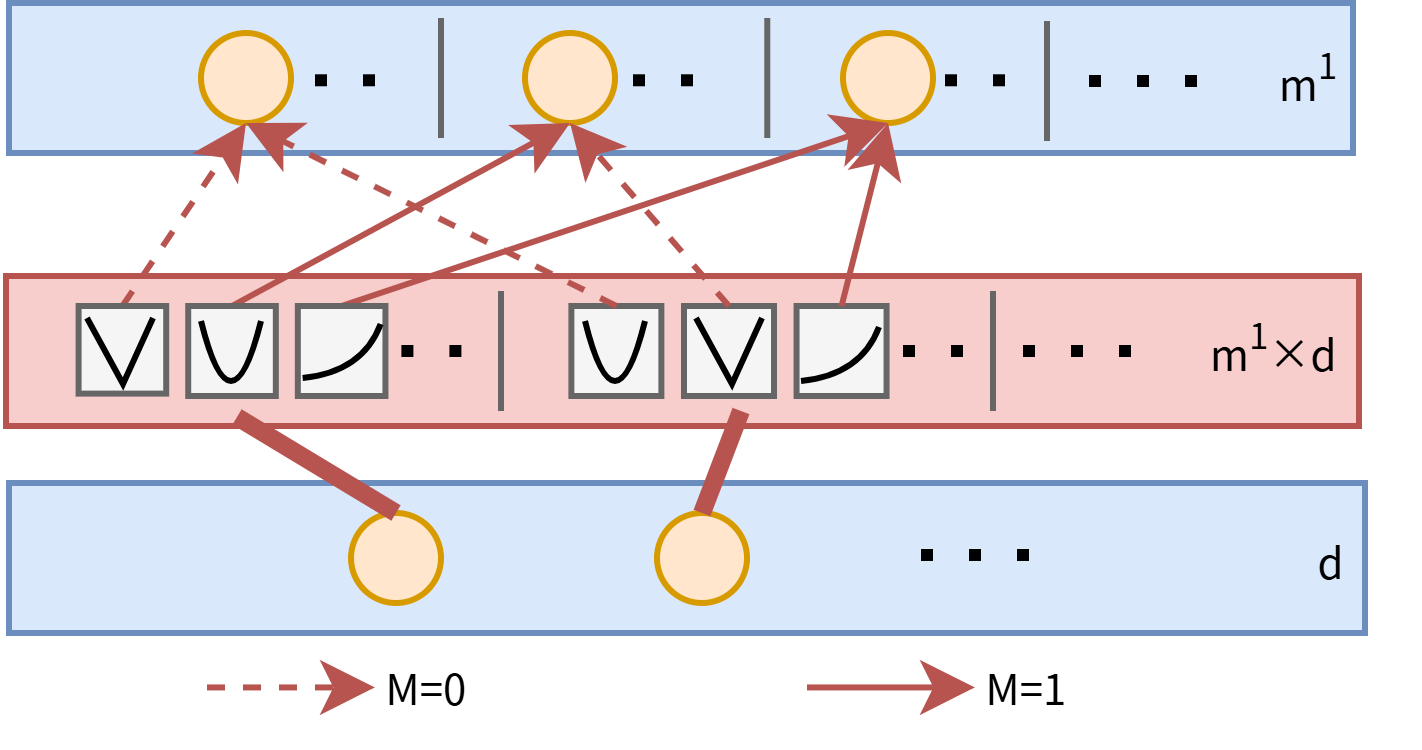
\includegraphics[width=0.7\linewidth]{figures/4.2Embedding_Causal_Knowledge.png}
	\caption{
		Causal-KAN第一层的知识融合结构。整体分为三层：底部是$d$个输入节点，中间是粉色的$m^1 \times d$掩码激活单元（带专属功能符号），顶部是$m^1$个输出预测节点。实心箭头（$M=1$）代表因果父变量与激活单元之间的有效连接，虚线箭头（$M=0$）代表非因果输入不参与后续计算，直接绕过激活单元。
	}
	\label{fig:Embedding_Causal_Knowledge}
\end{figure}

\subsection{局部连接激活层设计}

局部连接激活层是Causal-KAN的输出映射部分，主要作用是根据上层特征生成最终预测结果，同时保证各个因果机制之间互不干扰。如图~\ref{fig:local_layer_arch}所示，该层对上层输出的特征信息进行针对性处理，将维度为$m^{l-1} \times d$的输入转换为$m^{l+1}$维输出。
\begin{figure}[H]
	\centering
	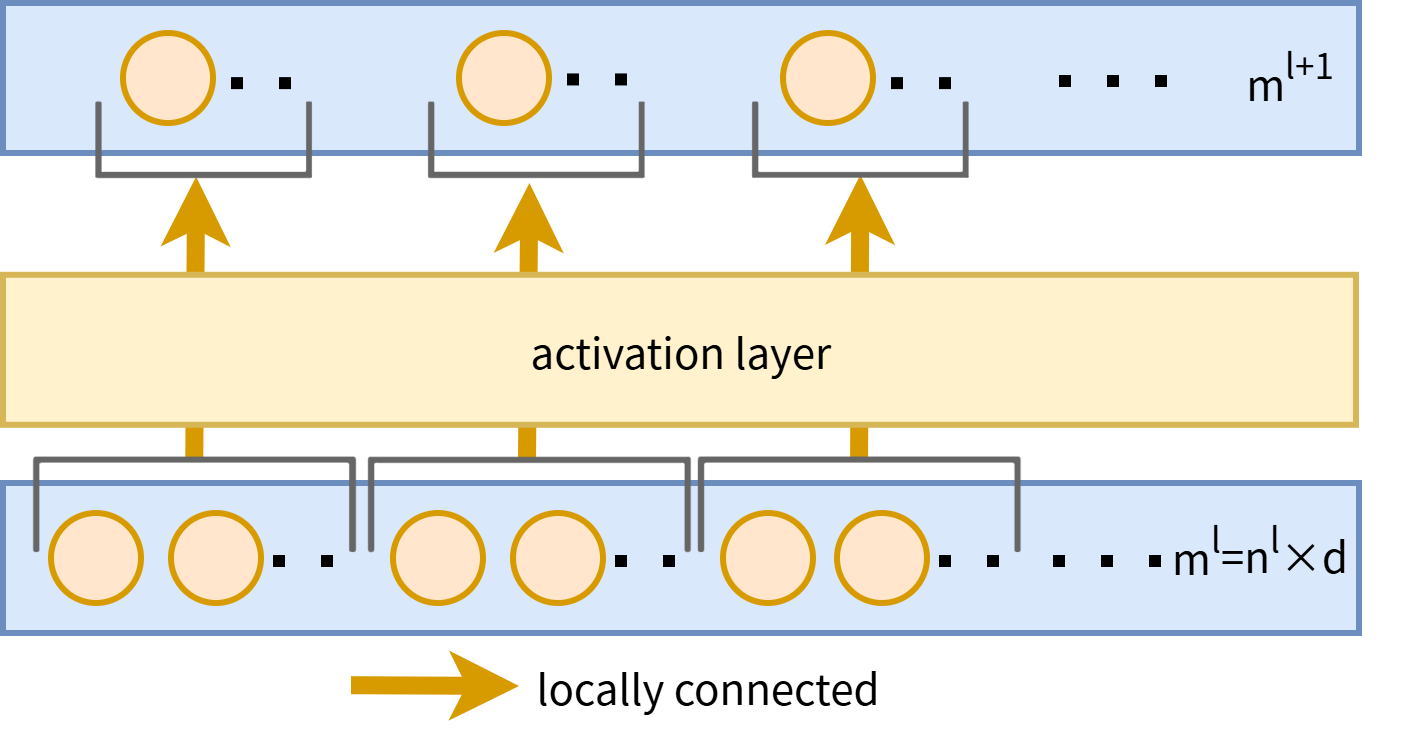
\includegraphics[width=0.7\linewidth]{figures/4.3locally_connection.png}
	\caption{局部连接激活层结构（黄色区域）。该层将维度为$m^{l-1} \times d$的输入特征转换为$m^{l+1}$个输出。实线代表有效计算路径，每条路径对应独立的激活函数$\eta_i$；虚线代表输入被绕过，不参与当前计算，以此保持各因果机制相互独立。}
	\label{fig:local_layer_arch}
\end{figure}


针对每一个输出变量$Y_i$，计算方式定义为：
\begin{equation}
	\hat{Y}_i = \eta_i\left( \sum_{k \in \mathcal{C}_i} w_{i,k} \cdot H_k \right)
\end{equation}
其中，$\mathbf{H}_i \in \mathbb{R}^{m}$为上层输出的隐藏特征，$\mathcal{C}_i \subseteq \{1,\dots,m\}$是为$Y_i$指定的特征子集，$w_{i,k}$为可学习权重，$\eta_i$为独立的样条激活函数。
该结构可以保证，当$k \notin \mathcal{C}_i$时，满足$\partial \hat{Y}_i / \partial H_k = 0$。与全连接层相比，这种方式能够有效保持不同因果机制之间的隔离性。

局部连接激活层在保持因果关系方面具备三项稳定特性：
第一，机制局部性。每个激活函数$\eta_i$仅作用于指定的特征子集$H_k \in \mathcal{C}_i$，如图~\ref{fig:local_layer_arch}中实线连接所示，避免不同机制之间出现信息串扰。
第二，模块独立性。每个$\eta_i$对应的样条参数$\{\beta^{(i)}_q\}$均可独立优化，使不同因果机制保持各自的函数关系，不产生交叉影响。
第三，结构隔离性。无关输入通过虚线箭头直接绕过当前计算单元，在保持局部依赖关系的同时，保留正常的梯度传播路径。

该层按照固定流程完成计算。
首先进行输入划分，根据因果约束将上层特征$\mathbf{H}_i$分配到对应的子集$\mathcal{C}_i$；
随后执行局部聚合，对相关特征进行加权求和，对应图中的$\oplus$运算；
接着通过独立激活函数完成非线性变换，形式为$\eta_i(z) = \sum_{q} \beta^{(i)}_q b_q(z)$；
最后实现输出隔离，将当前变量的预测结果$\hat{Y}_i$与其他机制解耦，避免相互干扰。
整体计算可表示为维度变换：$\mathbb{R}^{m^{l-1} \times d} \xrightarrow{} \mathbb{R}^{m^{l+1}}$。
通过禁止不同激活函数之间共享参数，模型满足独立因果机制原则，同时允许各机制的复杂度根据实际需求独立扩展。

\subsection{基于KAN的知识融合因果发现算法框架}
\label{sec:framework}
本节提出基于知识嵌入的函数因果图学习算法，利用变量观测数据 $\mathbf{X} = (X_1, \dots, X_d)$，通过Causal-KAN网络同时学习因果图结构与因果结构方程 $f_i$。在学习过程中，可以引入已有的领域因果知识，部分或全部确定变量间的因果方向，提升学习结果的可靠性。

如图~\ref{fig:causal_kan_arch}所示，Causal-KAN为每个输出变量 $Y_i$ 构建独立的网络分支，用于学习父变量 $\mathrm{PA}_i$ 到目标变量的映射关系。整个网络由三个基础部分构成：
\begin{figure}[H]
	\centering
	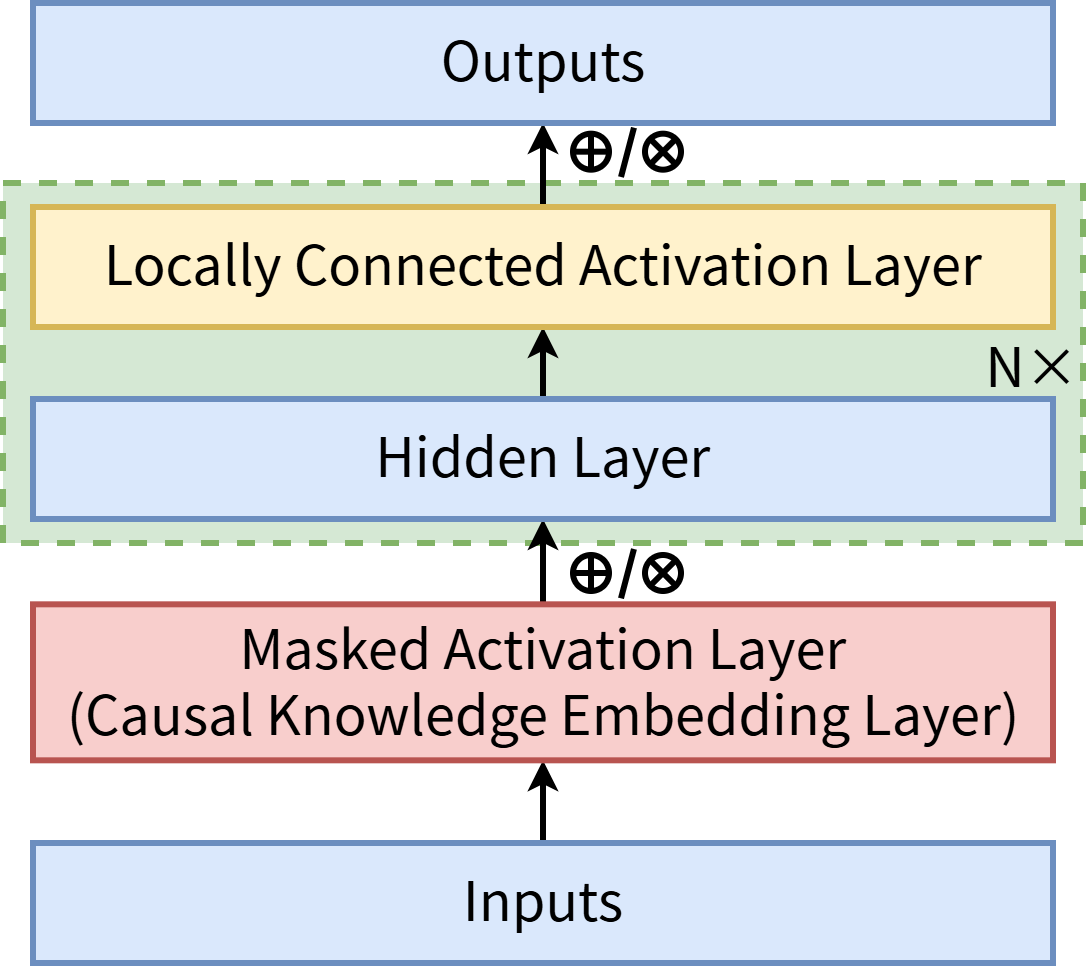
\includegraphics[width=0.7\linewidth]{figures/4.1masked_kan_structure.png}
	\caption{Causal-KAN整体架构。该架构分为三层结构：底层为因果知识嵌入层（粉色掩码激活层），中间为可选堆叠隐藏层（浅蓝色），顶层为局部连接输出层（黄色），可在因果约束下完成因果结构与函数的联合学习。}
	\label{fig:causal_kan_arch}
\end{figure}


\begin{compactenum}
	\item 掩码激活层：位于网络最底层，通过二进制掩码 $\mathbf{M}_i \in \{0,1\}^d$ 限制输入连接，仅允许因果父变量 $X_j \in \mathrm{PA}_i$ 进入后续计算，将因果知识直接嵌入网络结构。
	\item 隐藏层：为可选结构，通过求和、乘积等运算对中间特征进行处理，可根据数据复杂度堆叠多层，用于拟合变量间的复杂交互关系。
	\item 局部连接激活层：作为输出层，为每个目标变量设置独立的激活函数与计算路径，在生成预测值 $\hat{Y}_i$ 的同时，保证不同因果机制相互独立。
\end{compactenum}

该算法包含两种学习方式：局部因果模型学习与全局因果模型学习。一是局部因果模型学习。如果只需要关注部分变量的因果关系（比如只研究某个特定变量的影响因素），可以采用这种模式。此时模型针对单个变量 $Y_i$构建独立的预测分支，所有分支共享底层的掩码输入层，既保证了因果约束的一致性，又能节省计算资源。二是全局因果模型学习。如果需要构建完整的因果图（比如分析一个系统中所有变量的相互影响），则采用这种模式。此时模型同时学习所有变量的结构方程，网络中的中间节点代表内生变量（既作为其他变量的父变量，又作为某些变量的子变量），通过统一优化完成完整因果图的估计。通过这一计算过程，掩码机制能严格保证：非父变量 $X_j \notin \mathrm{PA}_i$ 对输出 $\hat{Y}_i$ 不存在任何影响，即满足 $\frac{\partial \hat{Y}_i}{\partial X_j} \equiv 0$，实现严格的因果隔离，确保每个变量的因果关系都不受无关变量干扰。

对于具有父节点 $\mathrm{PA}_i$ 的输出变量 $Y_i$，其基础计算过程如下：
\begin{equation}
	\begin{split}
		\hat{Y}_i &= g_i \Big( \sum_k \psi_k^{(out)} \Big( \sum_{j \in \mathcal{P}_i} \phi_{j}^{(masked)}(X_j) \Big) \Big)\\
		\mathcal{P}_i &= \{j: \mathbf{M}_{i,j}=1\}
	\end{split}
\end{equation}
式中，$\phi^{(masked)}(X_j)$ 是输入变量 $X_j$ 经过掩码激活层处理后的特征值，非因果父变量的特征值在此步已被屏蔽为0；$\psi_k^{(out)}$ 是隐藏层的特征变换函数，对应层内的求和、乘积等聚合运算；$g_i$ 是局部连接激活层的输出激活函数，与前面提到的 $\eta_i$ 一致，通常为B-样条函数；$\mathcal{P}_i$ 是 $Y_i$ 的因果父变量集合，由掩码 $\mathbf{M}_i$ 直接确定（掩码值为1的变量构成该集合）。

\label{sec:training_algorithm}

Causal-KAN采用多阶段训练方式，将因果结构约束与函数优化结合，完整的训练流程如算法~\ref{alg:causal-kan}所示。

整个训练过程可以分为两个阶段：
第一阶段是掩码初始化与嵌入，核心是将先验因果知识转化为网络的结构约束。首先根据已知的因果关系生成原始掩码矩阵$M_{\text{pre}}$，然后根据各层网络的宽度的维度，将原始掩码扩展为适配的格式\pozhehao 输入层直接使用扩展后的因果掩码，确保非因果变量被过滤；隐藏层采用扩展后的掩码，保证各变量的计算路径相互独立，避免跨变量的信息干扰。通过这一步，因果知识被完全嵌入网络结构，后续训练不会改变这些约束。第二阶段是模型优化。我们选择LBFGS优化器进行训练，主要因为它在拟合光滑函数时效率更高、收敛更稳定。训练过程中设置了80轮迭代，同时开启动态网格更新，这意味着模型会根据数据的分布特点，自动调整B-样条的网格密度，让函数拟合更精准。需要说明的是，这里没有添加额外的正则化项（$\lambda=0$），因为掩码层已经从结构上实现了参数稀疏性约束，非因果路径的参数不会被更新，无需再通过正则化压缩参数。最终，模型输出两部分核心结果：一是完整的因果图结构（由掩码矩阵和修剪后的连接关系共同确定，明确变量间的因果边及方向）；二是各变量对应的因果函数${f_i}$图像，实现了因果结构与因果函数的联合学习。
\begin{algorithm}[H]
	\caption{基于结构约束的Causal-KAN训练流程}
	\label{alg:causal-kan}
	\begin{algorithmic}[1]
		\REQUIRE 因果掩码矩阵 $M_{\text{pre}} \in \{0,1\}^{d \times d}$, 训练集 $\mathcal{D}_{\text{train}}$，测试集 $\mathcal{D}_{\text{test}}$,  网络宽度参数 $\mathbf{w} = [w_0, [w_{1a}, w_{1b}], w_2]$ , 样条网格参数 $(N_{\text{grid}}, k)$
		\STATE \textbf{网络初始化}
		\STATE 构建基础KAN网络：$\mathcal{M} \leftarrow \text{KAN}(\mathbf{w}, N_{\text{grid}}, k, \text{mult\_arity}=[0, \mathbf{m}, 0])$
		\STATE \textbf{因果掩码嵌入}
		\FOR{网络层 $l = 0$ to $\text{depth}(\mathcal{M})-1$}
		\IF{$l = 0$}
		\STATE 扩展输入层掩码：$M_1 \leftarrow \text{repeat}(M_{\text{pre}}, \lfloor w_{1a}/d \rfloor, \text{dim}=1)$
		\STATE 掩码维度扩展：$M_2 \leftarrow \text{expand\_mask}(M_{\text{pre}})$
		\STATE 为输入层激活函数设置掩码：$\mathcal{M}.\text{act\_fun}[l].\text{mask} \leftarrow [M_1; M_2]^T$
		\ELSE
		\STATE 构建单位掩码并隔离目标变量：$M_I \leftarrow \mathbb{I}_d$
		\STATE 掩码扩展与重排：$M_{\text{ext}} \leftarrow \text{repeat\_interleave}(M_I, \text{factors}=[\lfloor w_l/d \rfloor, \lfloor w_{l+1}/d \rfloor])$
		\STATE 为隐藏层激活函数设置掩码：$\mathcal{M}.\text{act\_fun}[l].\text{mask} \leftarrow M_{\text{ext}}$
		\ENDIF
		\ENDFOR
		\STATE \textbf{模型优化与修剪}
		\STATE 预训练网络：$\mathcal{M}.\text{fit}(\mathcal{D}_{\text{train}}, \text{opt}=\text{"LBFGS"}, T=80, \lambda=0, \text{update\_grid}=\text{True})$
		\STATE \textbf{输出结果}
		\STATE 得到各因果机制对应的符号函数 $\{f_i\}$
	\end{algorithmic}
\end{algorithm}

综上，Causal-KAN 的模型构建通过分层模块化设计，解决了因果知识融合与非线性因果函数拟合的核心问题。知识融合层以二进制掩码为核心，将因果约束直接转化为网络结构，从根源上屏蔽非因果变量的干扰，保证了因果依赖的忠实性；局部连接激活层通过独立机制建模，避免了不同因果函数间的交叉影响，契合独立因果机制原则；算法框架则整合两层核心结构，支持局部与全局两种学习模式，同时通过多阶段训练流程，实现了因果结构与函数的联合优化。

\section{实验验证}
\label{sec:sachs_experiments}
为全面验证 Causal-KAN 模型的性能，本章节设计了模拟数据实验与真实数据实验两部分验证方案。模拟数据实验通过控制变量法，在已知因果骨架的前提下，重点评估模型的函数拟合精度、抗过拟合能力、可扩展性及计算效率，排除结构学习误差的干扰，纯粹检验模型本身的表达与正则化特性；真实数据实验则采用 Sachs 蛋白质信号网络数据集，依托其已知的因果结构作为标准，验证模型在实际场景中的适用性，同时分析学习到的因果映射的可解释性与生物学意义。两类实验从不同维度相互补充，形成完整的性能验证体系，确保评估结果的全面性与可靠性。

\subsection{模拟数据实验设置}{\label{subsec:exp_setup}}

{\hei 1.数据集构建}{\label{subsubsec:data_construction}}

本次实验用基于结构因果模型（SCM）生成的合成数据，核心目的是在已知因果图骨架的前提下，专门评估Causal-KAN的两个关键性能：一是对非线性因果函数的拟合能力，二是抵抗过拟合的能力，避免结构学习的误差干扰对模型本身性能的判断。

变量配置：实验共设置四种节点规模 $d \in \{10, 20, 30, 40\}$，以考察算法在不同维度下的可扩展性（Scalability）。噪声水平设置为 $\sigma \in \{0.1, 0.2, 0.3\}$，用于检验模型在观测噪声干扰下的鲁棒性（Robustness）。所有实验固定样本量为 $n=1000$。

图结构生成：因果图主要采用埃尔德什$\-$雷尼（Erdős–Rényi, ER）随机图模型生成，边数倍数设为 $m=2$，即期望边数为 $|\mathcal{E}| = m \times d$。例如，当 $d=20$ 时，图中包含约 40 条有向边。该设置旨在模拟中等稀疏程度的真实因果网络。

因果函数设计：结构方程中的因果函数采用嵌套初等函数形式（2 层复合），即 $f_j(\text{Pa}_j) = g_2(g_1(\text{Pa}_j))$，其中 $g_1, g_2$ 从正弦、指数、多项式等初等函数集中随机选取。该设计用于模拟真实场景中普遍存在的非线性、非加性因果映射关系。

先验知识设置：先验知识全部覆盖，表示因果邻接矩阵完全已知。该设定的设计意图在于：隔离结构学习误差的干扰，单独评估模型在给定正确骨架下的函数拟合精度与泛化能力，从而更清晰地刻画模型本身的表达与正则化特性。

重复实验与随机性控制：为了减少单次实验的随机波动带来的误差，每种配置（$d$, $\sigma$ 组合）下独立运行 5 次实验，随机种子固定为 $\{2, 4, 6, 8, 10\}$。最终结果以均值±标准差形式报告。实验共完成 60 组独立训练任务。

{\hei 2.评价指标}{\label{subsubsec:evaluation_metrics}}

实验从四个维度设计评价指标，全面评估模型性能，分别是函数拟合精度、模型复杂度、网络稀疏度和计算效率。


（1）函数拟合精度
核心用两个指标衡量模型对因果函数的拟合效果：均方误差（MSE）与决定系数（$R^2$）作为核心评价指标，计算都基于测试集数据：
\begin{equation}
	\text{MSE} = \frac{1}{n_{\text{test}}}\sum_{i=1}^{n_{\text{test}}}(\hat{y}_i - y_i)^2, \quad 
	R^2 = 1 - \frac{\sum(\hat{y}_i - y_i)^2}{\sum(y_i - \bar{y})^2}
\end{equation}
其中 $\hat{y}_i$ 为模型预测值，$y_i$ 为真实观测值。同时记录训练集与测试集 $R^2$ 的差值作为泛化间隙，用于间接评估过拟合程度。

（2）模型复杂度
记录三项参数指标：
\begin{itemize}
	\item 总参数量：网络中所有可学习参数的总数；
	\item 可训练参数量）：实际参与梯度更新的参数数量；
	\item 模型存储大小：以 MB 为单位的参数字节占用。
\end{itemize}
不同节点规模下的模型复杂度如表~\ref{tab:model_complexity} 所示。

\begin{table}[htbp]
	\centering
	\caption{不同节点规模下的模型复杂度统计}{\label{tab:model_complexity}}
	\begin{tabular}{cccc}
		\toprule
		节点数 $d$ & 总参数量 & 可训练参数量 & 模型大小 (MB) \\
		\midrule
		10  & 15,560  & 13,300  & 0.059 \\
		20  & 60,520  & 53,200  & 0.231 \\
		30  & 134,880 & 119,700 & 0.515 \\
		40  & 238,640 & 212,800 & 0.910 \\
		\bottomrule
	\end{tabular}
\end{table}

（3）网络稀疏度
为量化正则化对结构剪枝的效果，分别统计两层连接的实际激活比例：
\begin{itemize}
	\item 第 0 层（输入→掩码激活层）：理论最大边数为 $d \times d \times m$，记录实际非零连接数及稀疏度 $\text{Sparsity} = 1 - \frac{\text{active\_edges}}{\text{total\_edges}}$；
	\item 第 1 层（掩码激活层→输出）：同理计算。
\end{itemize}
不同配置下的稀疏度统计如表~\ref{tab:sparsity} 所示。

\begin{table}[htbp]
	\centering
	\caption{不同节点规模下的网络稀疏度统计}{\label{tab:sparsity}}
	\begin{tabular}{ccccc}
		\toprule
		\multirow{2}{*}{$d$} & \multicolumn{2}{c}{第 0 层} & \multicolumn{2}{c}{第 1 层} \\
		\cmidrule(lr){2-3} \cmidrule(lr){4-5}
		& 总边数 & 稀疏度 & 总边数 & 稀疏度 \\
		\midrule
		10 & 400  & 0.850 & 300  & 0.900 \\
		20 & 1600 & 0.925 & 1200 & 0.950 \\
		30 & 3600 & 0.950 & 2700 & 0.967 \\
		40 & 6400 & 0.963 & 4800 & 0.975 \\
		\bottomrule
	\end{tabular}
\end{table}


（4）计算效率
记录单次实验的训练耗时（单位：秒），在相同硬件环境（Intel Core i9-14900K CPU）下测量，用于评估算法的实际部署成本。

\subsection{模拟数据实验结果与分析}{\label{subsec:simu_results}}

{\hei 1.整体性能汇总}{\label{subsubsec:overall_summary}}

表~\ref{tab:summary_stats} 汇总了全部 60 组实验的核心指标统计结果。测试集 $R^2$ 均值为 0.613（标准差 0.081），说明在给定正确因果骨架的情况下，Causal-KAN能有效拟合非线性的因果函数；测试集MSE的均值是0.383，而且随着噪声水平升高，MSE会跟着单调增长，这和预期一致——噪声越大，拟合误差自然会变大。训练时间的均值是46.31秒，标准差26.64秒，耗时范围在10.73秒到92.58秒之间，整体计算效率处于合理水平。

\begin{table}[htbp]
	\centering
	\caption{实验指标汇总统计（60 组实验）}{\label{tab:summary_stats}}
	\begin{tabular}{lccc}
		\toprule
		指标 & 均值 & 标准差 & 取值范围 \\
		\midrule
		MSE  & 0.383 & 0.077 & [0.204, 0.633] \\
		$R^2$ & 0.613 & 0.081 & [0.353, 0.794] \\
		训练时间 (s) & 46.31 & 26.64 & [10.73, 92.58] \\
		\bottomrule
	\end{tabular}
\end{table}

{\hei 2.噪声水平对拟合性能的影响}{\label{subsubsec:noise_analysis}}

表~\ref{tab:noise_analysis}展示了不同噪声水平下的模型拟合性能。从表中能清楚看到，当噪声水平$\sigma$从0.1增加到0.3时，测试集$R^2$从0.674降到了0.563，测试集MSE从0.312升到了0.436。这个变化趋势很合理，说明模型对观测噪声的敏感性在正常范围内，既没有异常稳健（比如噪声增大误差不变），也没有过度敏感（比如噪声稍微变大误差就急剧上升）。
进一步分析泛化间隙发现，低噪声条件下（$\sigma=0.1$），训练集和测试集的$R^2$差异很小，均值只有0.012，说明模型没有明显过拟合；随着噪声增大，泛化间隙虽然略有上升，但在$\sigma=0.3$时也只有0.028，仍然在合理范围内。这说明Causal-KAN的$L_1$正则化和因果掩码机制起到了很好的作用，有效控制了模型复杂度，避免了过拟合。
\begin{table}[htbp]
	\centering
	\caption{不同噪声水平下的拟合性能对比}{\label{tab:noise_analysis}}
	\begin{tabular}{lcc}
		\toprule
		噪声水平 $\sigma$ & MSE (均值) & $R^2$ (均值) \\
		\midrule
		0.1 & 0.312 & 0.6745  \\
		0.2 & 0.399 & 0.594  \\
		0.3 & 0.436 & 0.563  \\
		\bottomrule
	\end{tabular}
\end{table}

{\hei 3.节点规模对可扩展性的影响}{\label{subsubsec:scalability_analysis}}

表~\ref{tab:scalability_analysis}是不同节点规模下的性能对比。从结果能看出，随着节点数$d$从10增加到40，测试集$R^2$基本保持稳定，在0.604到0.621之间波动，变化很小。这符合预期，因为在因果骨架已知的前提下，函数拟合任务主要依赖父变量和子变量之间的局部关系，对整体变量维度的敏感度不高，所以即使变量变多，拟合精度也不会明显下降。
\begin{table}[htbp]
	\centering
	\caption{不同节点规模下的性能对比}{\label{tab:scalability_analysis}}
	\begin{tabular}{lccc}
		\toprule
		节点数 $d$ & MSE & $R^2$ & 训练时间 (s) \\
		\midrule
		10 & 0.388 & 0.608 & 11.85 \\
		20 & 0.378 & 0.621 & 37.42 \\
		30 & 0.386 & 0.611 & 50.13 \\
		40 & 0.382 & 0.604 & 83.67 \\
		\bottomrule
	\end{tabular}
\end{table}

训练时间方面，随着节点规模增长呈超线性趋势：$d=10$时平均耗时11.85秒，$d=40$时达到83.67秒。这主要是因为节点增多后，参数矩阵的维度变大，梯度计算的开销也随之增加。但即便如此，在$d=40$这种中等维度下，单次实验的平均耗时仍然控制在84秒以内，说明Causal-KAN的轻量级单层架构计算效率不错，具备较好的可扩展性。

\subsection{真实数据实验设置}
本实验旨在评估Causal-KAN在Sachs蛋白质信号网络数据集上的表现，该数据集包含11个变量和746个观测值。数据集已知的因果结构（图\ref{fig:sachs_dag}）为验证提供了黄金标准。节点代表磷酸化蛋白（如Raf、Mek、Erk），连接线表示信号通路。不同粗细的线条用于表示变量间关联强度的差异。掩码激活层中$M_i$矩阵的初始化是该有向无环图（DAG）中的关键步骤。
\begin{figure}[H]
	\centering
	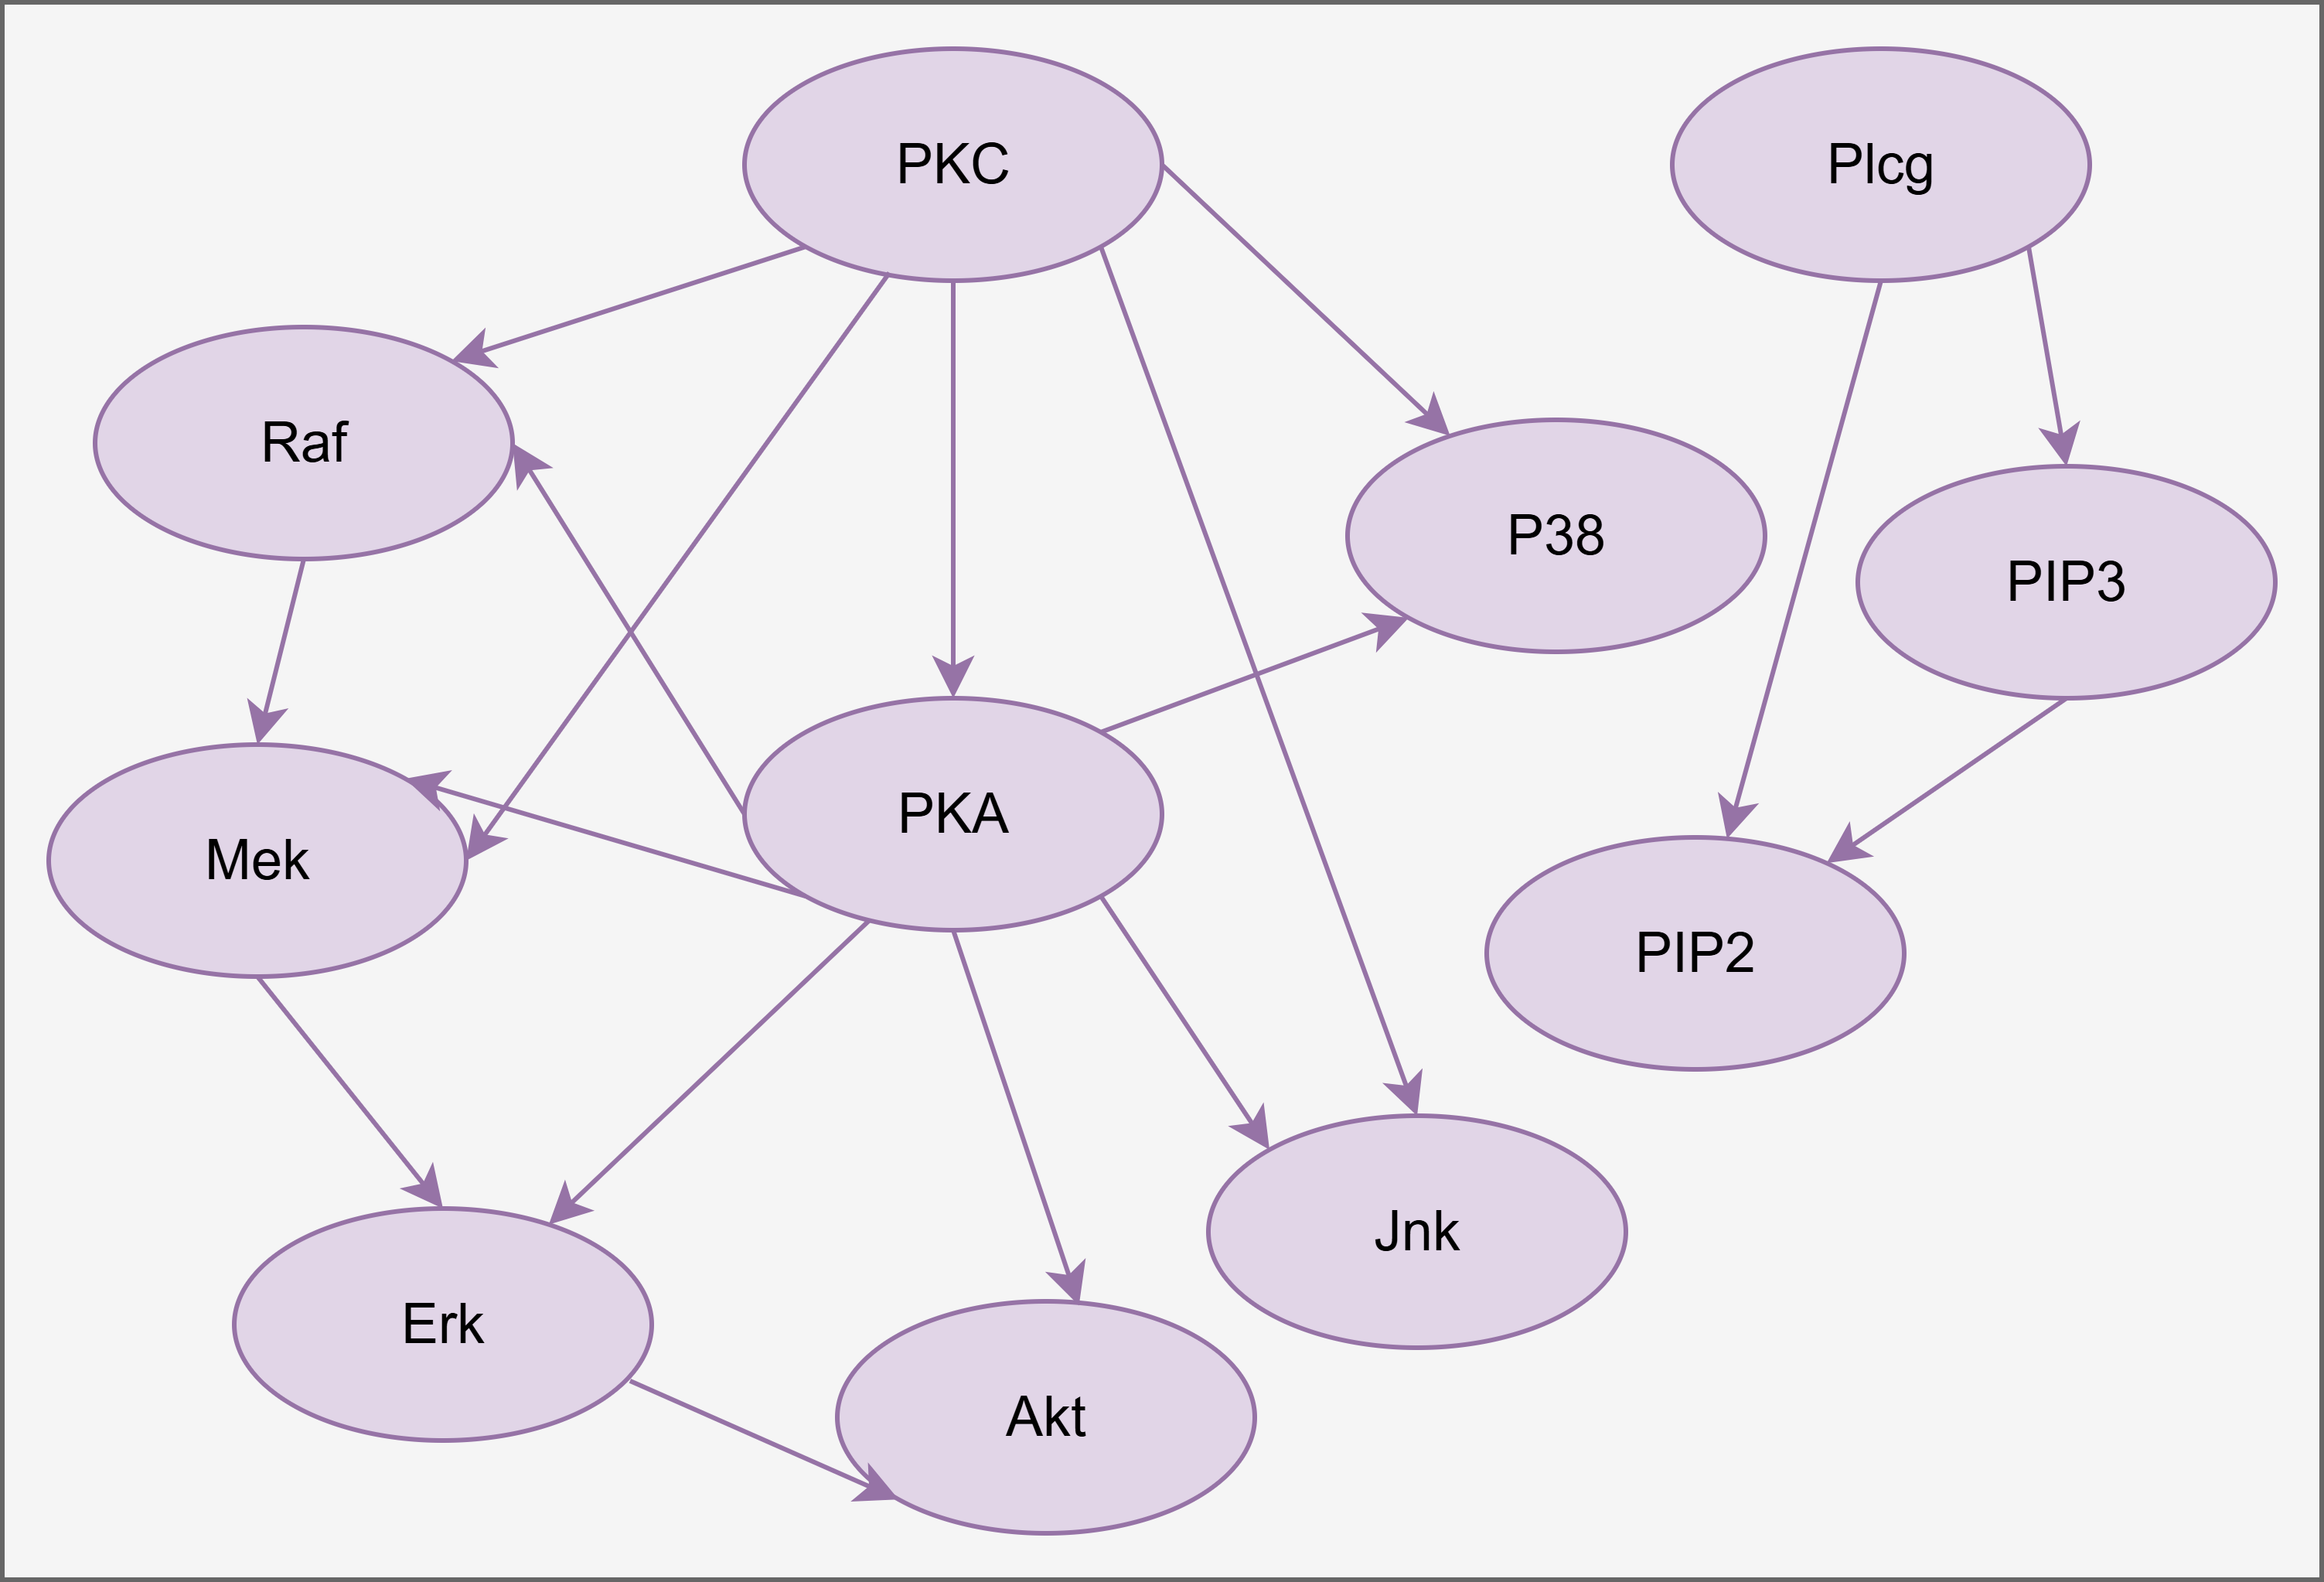
\includegraphics[width=0.7\linewidth]{figures/Sachs_dag.png}
	\caption{Sachs数据集的因果结构}
	\label{fig:sachs_dag}
\end{figure}

{\hei 1.数据集预处理}

实施了两步标准化流程：

1) 对数转换 缓解高度偏态分布 ($X' = \log(X+1)$)；

2) Z分值标准化 缩放数值 ($X_{\text{norm}} = \frac{X' - \text{mean}(X')}{\text{std}(X')}$)让每个变量的均值为0、标准差为1，避免不同变量的数值范围差异影响训练效果。

{\hei 2.初始化及参数设置}

如表~\ref{tab:hyperparams}所示，超参数配置遵循指定参数。
\begin{table}[H]
	\centering
	\caption{Sachs实验的超参数配置}
	\label{tab:hyperparams}
	\begin{tabular}{@{}lc@{}}
		\toprule
		参数 & 值 \\
		\midrule
		掩码激活初始化 & 使用图 \ref{fig:sachs_dag} 邻接矩阵 \\
		局部连接单元 ($\eta_i$) & 22 节点加 11 节点次方 \\
		网格尺寸 ($N_{\text{grid}}$) & 10 \\
		B样条阶数 $k$ & 3 \\
		\bottomrule
	\end{tabular}
\end{table}

掩码激活层采用图\ref{fig:sachs_dag}的邻接矩阵初始化，确保因果关系在结构中嵌入。本研究中，局部连接单元采用11+节点与11×节点配置，网格尺寸为10。初始化后的KAN结构（图\ref{fig:kan_structure}）通过底部垂直线建立输入连接，中部曲线路径表示激活通路，顶部节点簇体现输出分组，展现节点间的连接模式。
\begin{figure}[H]
	\centering
	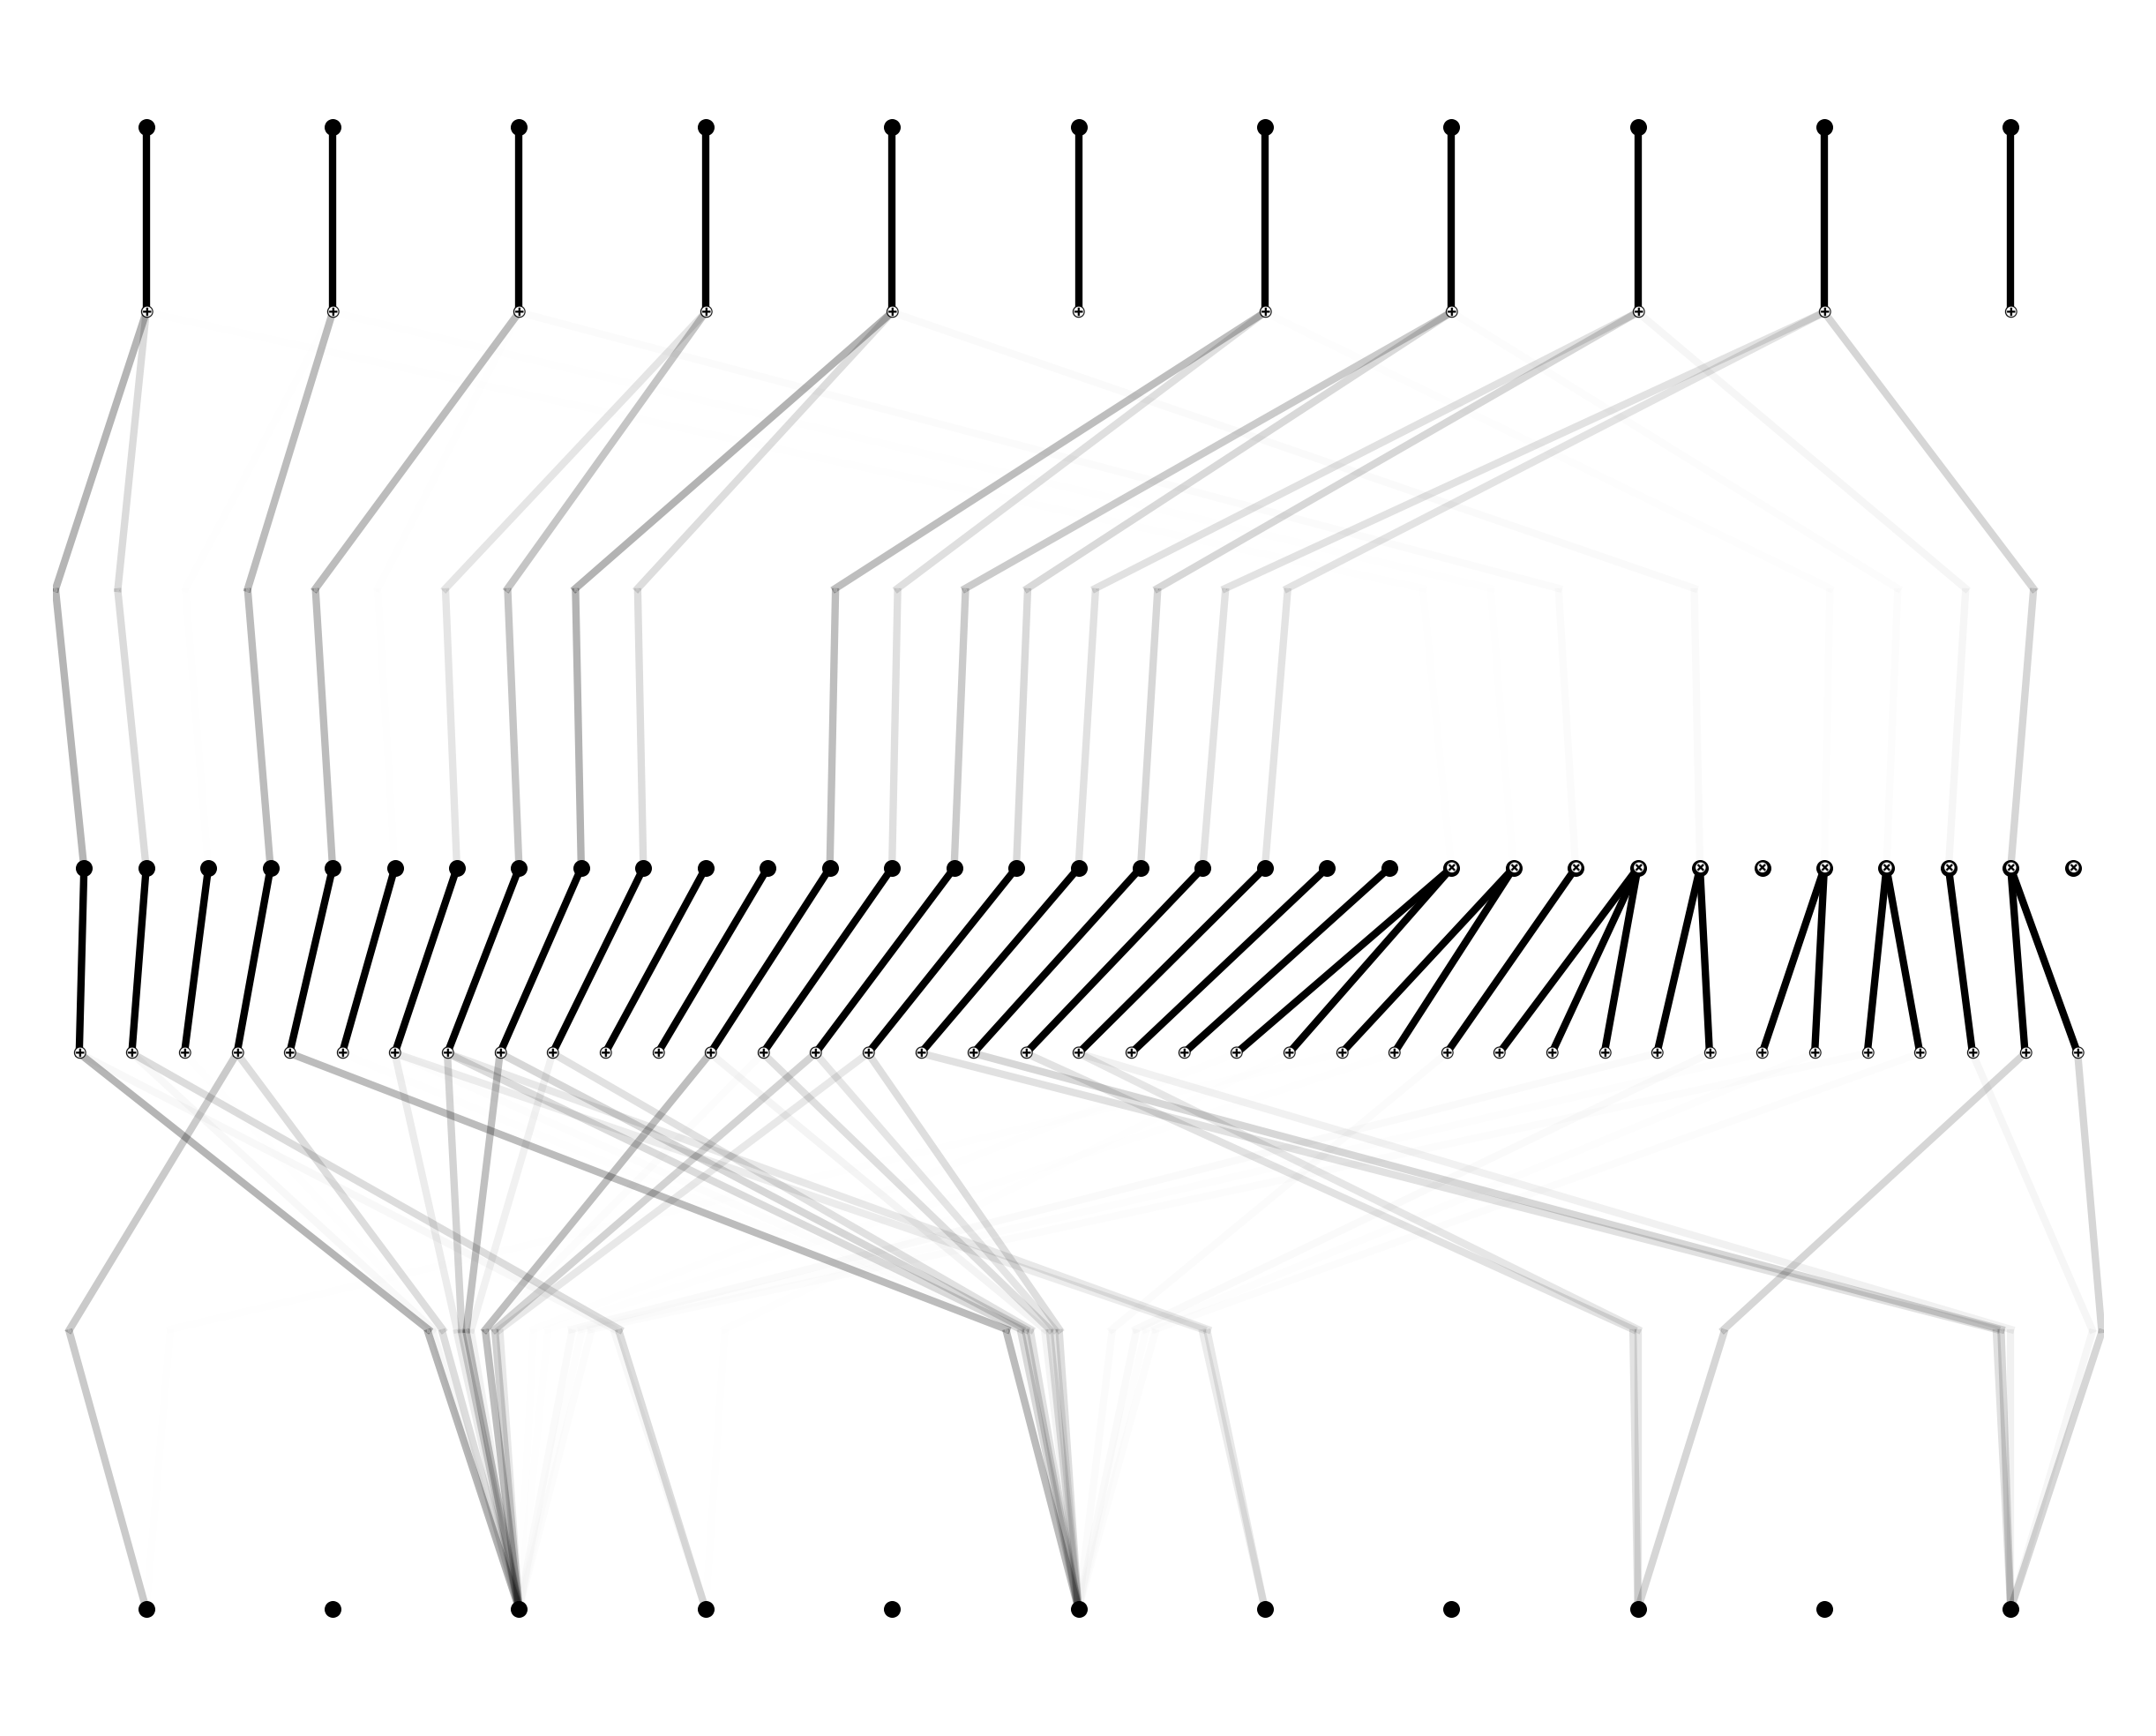
\includegraphics[width=0.97\linewidth]{figures/init.png}
	\caption{初始化后的KAN结构}
	\label{fig:kan_structure}
\end{figure}

\subsection{真实数据实验结果与分析}
图~\ref{fig:training_progress}展示了模型的训练进度，能看出明显的有效学习动态：带因果约束的模型（图\ref{fig:training_progress}b）在前20步训练中，损失就从0.64快速降到0.57，之后逐渐平稳，到第80步时基本收敛，测试损失稳定在0.59左右。
对比没有因果约束的模型（图\ref{fig:training_progress}a），能清楚看到因果知识嵌入的作用：无约束模型的训练损失最终稳定在$0.44\pm0.01$，测试损失是$0.52\pm0.02$，两者差距有0.08，存在明显的过拟合风险；而带因果约束的模型，训练损失稳定在$0.56\pm0.01$，测试损失稳定在$0.59\pm0.01$，泛化间隙很小。这说明即使Sachs数据集的样本量有限（仅746个），嵌入因果知识也能有效防止过拟合——因果掩码相当于一种结构性的正则化，限制了模型的搜索空间，避免模型学到数据中的噪声。
\begin{figure}[H]
	\centering
	\subfloat[无因果约束]{
		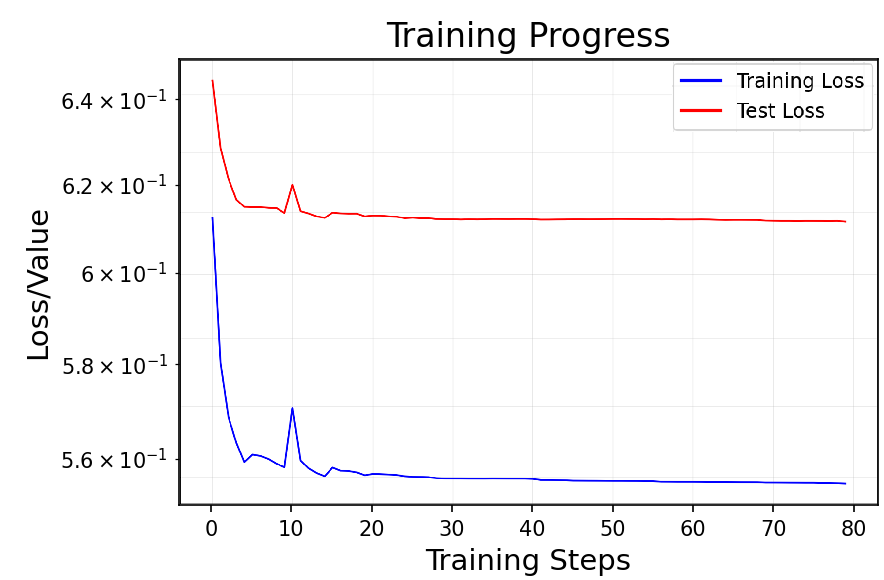
\includegraphics[width=0.46\linewidth]{figures/无约束loss.png}}
	\hfill
	\subfloat[带因果约束]{
		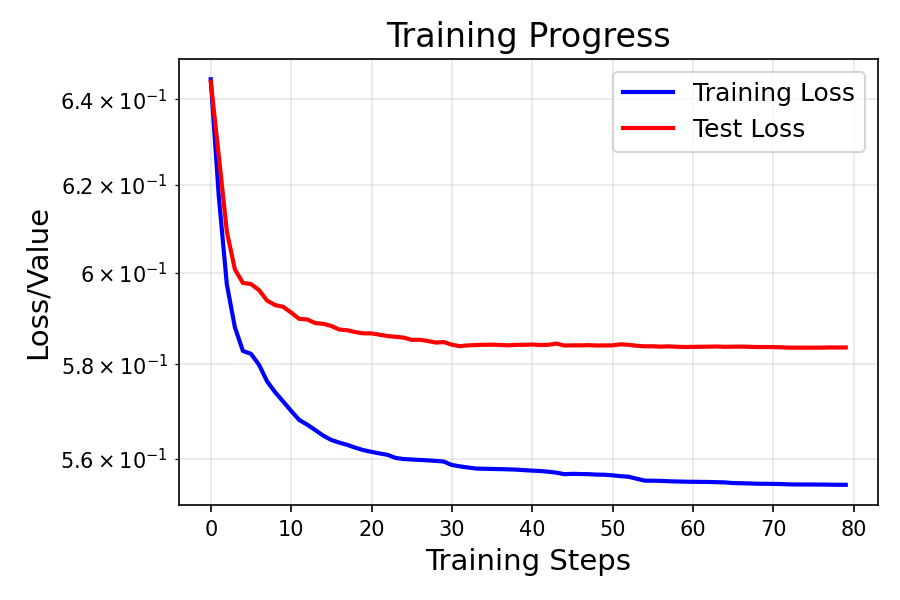
\includegraphics[width=0.46\linewidth]{figures/loss.png}}
	\caption{训练进度比较}
	\label{fig:training_progress}
\end{figure}

通过可视化Causal-KAN学习到的因果映射，发现前体分子PIP3/Plcg与靶分子PIP2之间存在独特的功能关系（如图\ref{fig:pathway_analysis}所示），而且不同通路对PIP2的调控作用差异很大，具体可以从三个方面分析：
\begin{compactenum}
	\item 通路斜率差异: 左通路（$X_{1.0}\rightarrow$PIP2）显示最小斜率（$\beta_{1,0} = 0.02$）； 中央通路（$X_{1.1}\rightarrow$PIP2）呈现强线性关系（$\beta_{1,1} = 0.81$）；右侧通路（$X_{1.2}\rightarrow$PIP2）在限定范围内（$\Delta y = 0.03$）呈现高频波动。
	\item 对输出变异的影响范围: 不同通路对PIP2输出变异幅度的影响存在显著差异（$\Delta y_{X_{1.1}} = 0.38$ vs $\Delta y_{X_{1.2}} = 0.03$）。
	\item 功能意义: 中央通路的输入$X_{1.1}$能解释PIP2 78\%的方差（$R^2=0.78$），而左通路（$X_{1.0}$）和右侧通路（$X_{1.2}$）的贡献极小，$R^2$分别只有0.02和0.07。
\end{compactenum}
\begin{figure}[H]
	\centering
	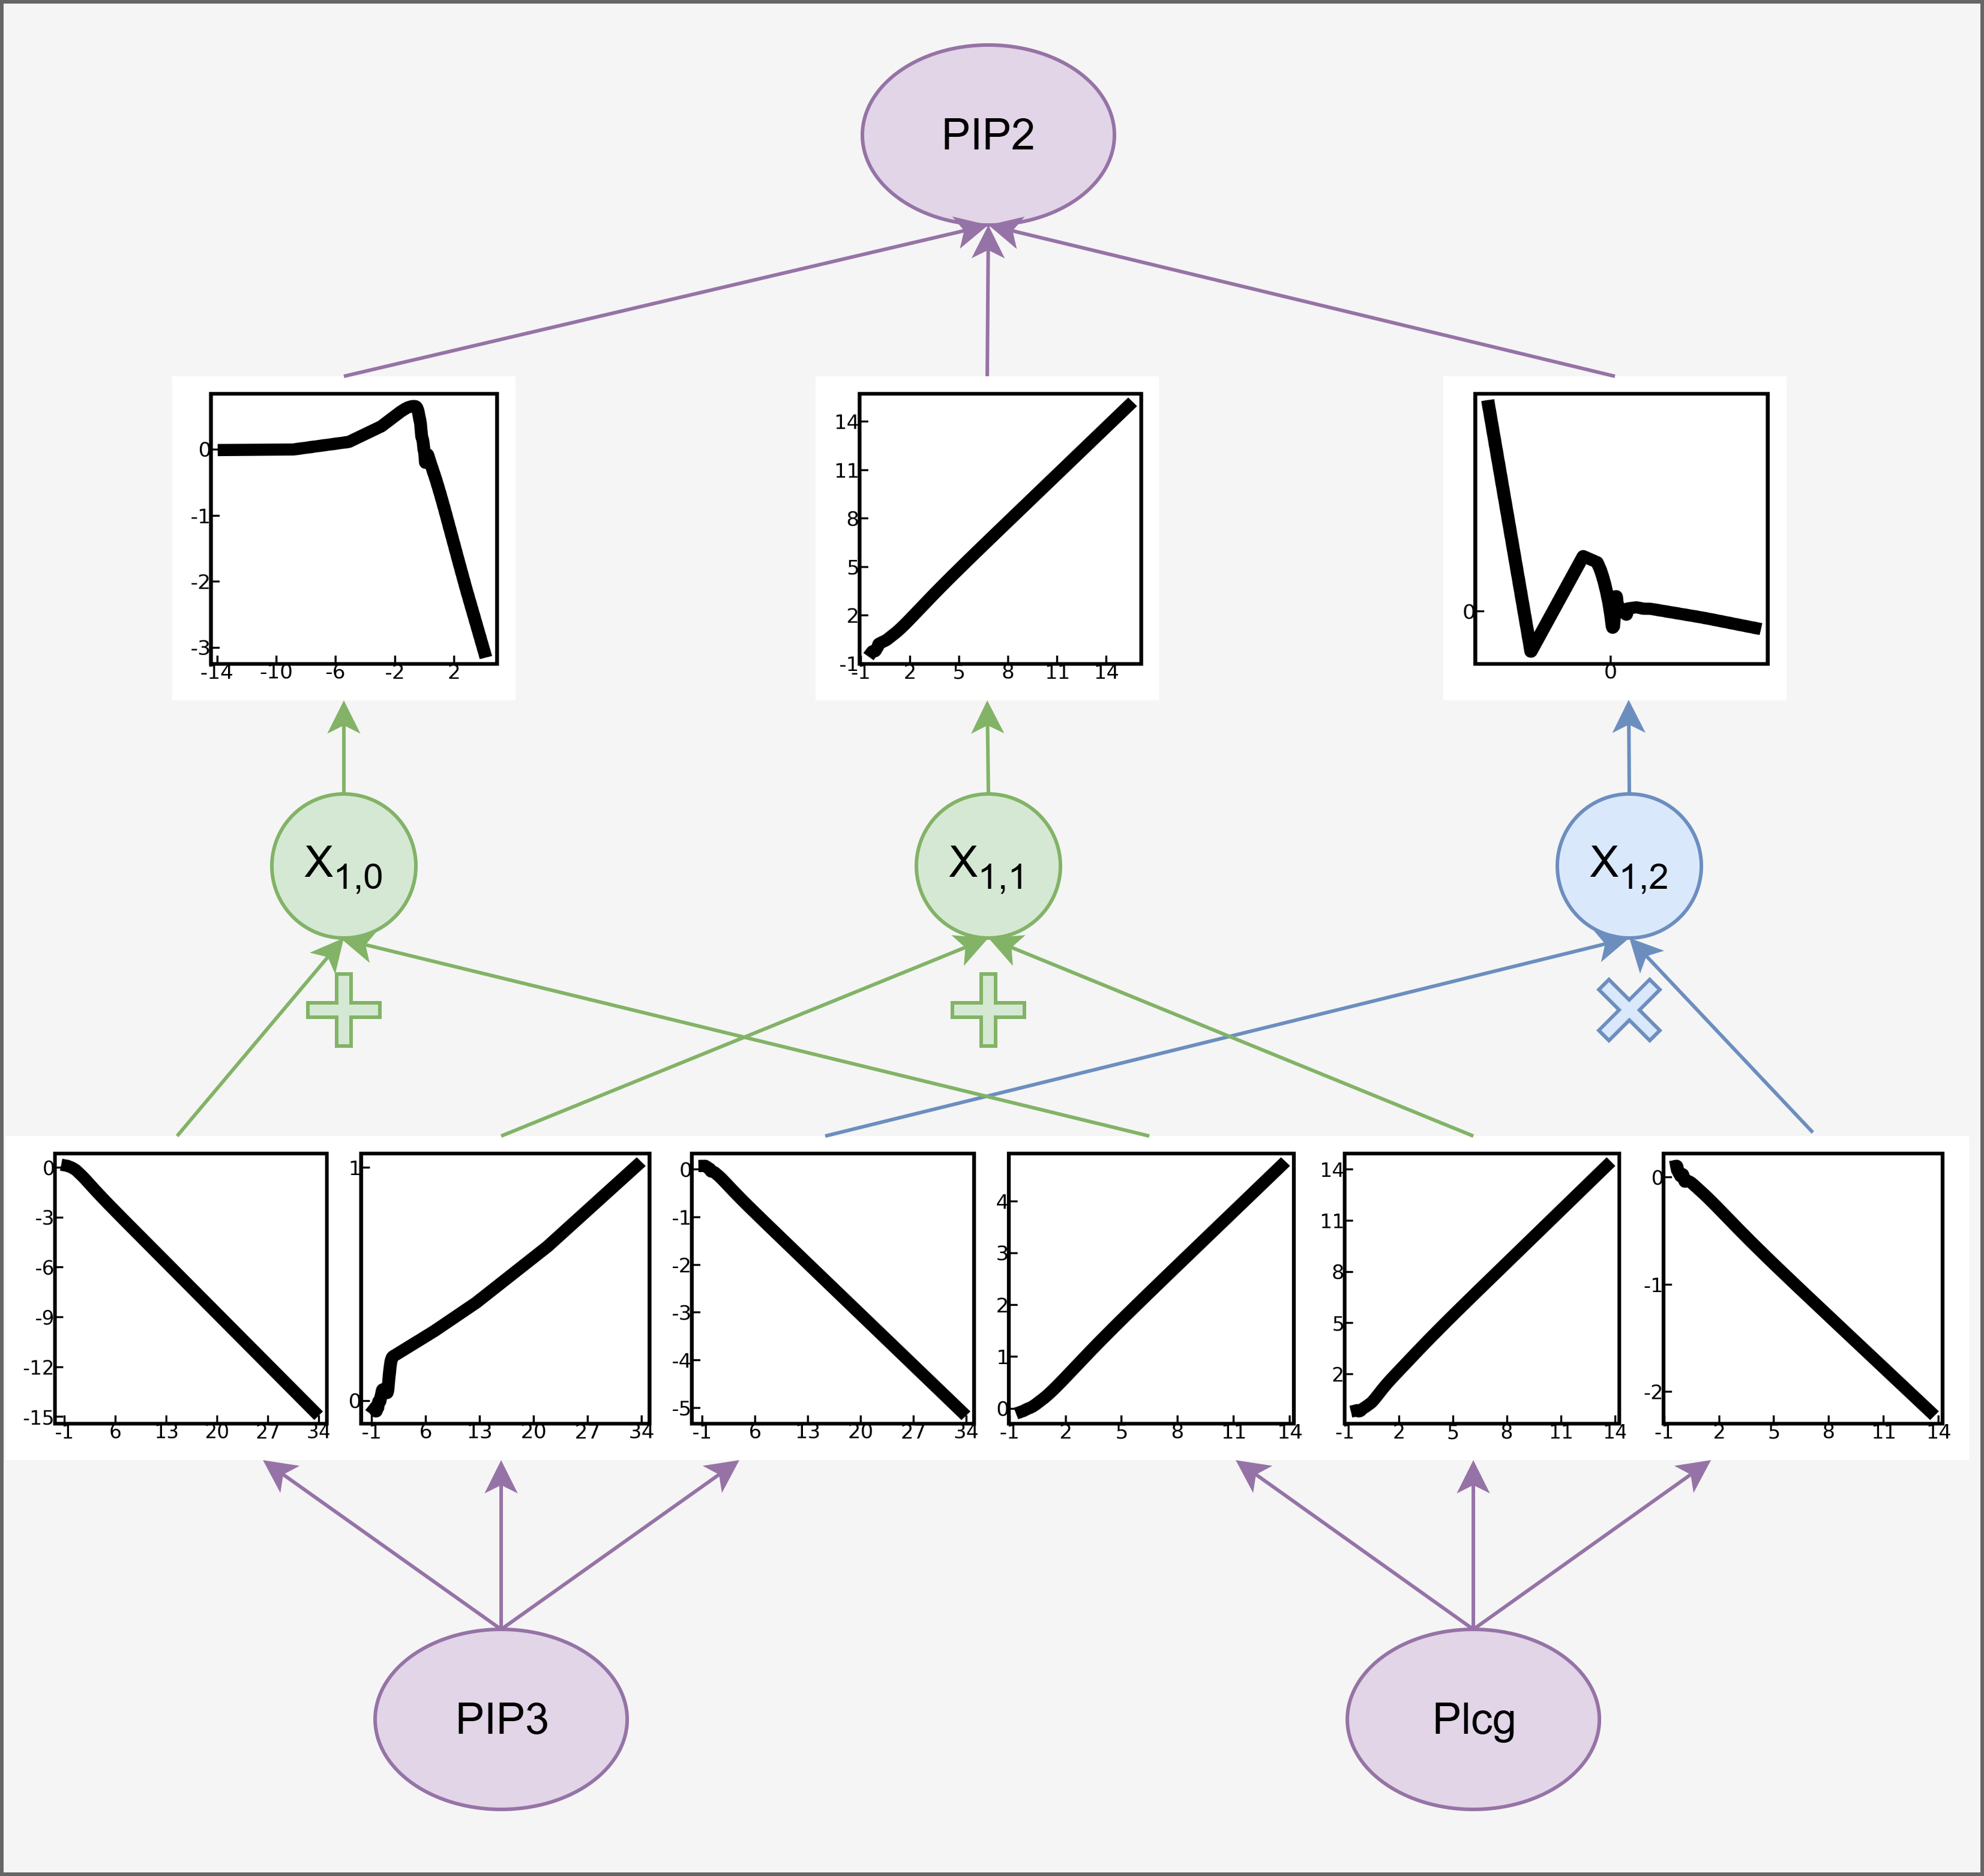
\includegraphics[width=0.5\linewidth]{figures/Sachs_PIP2.png}
	\caption{PIP2调控中各通路的差异贡献}
	\label{fig:pathway_analysis}
\end{figure}

定量分析进一步证实，加法节点$X_{1.1}$构建了PIP2调控的主要通道：其斜率$\beta=0.81\pm0.05$（p<0.001），统计显著；而左通路$X_{1.0}\rightarrow$PIP2的映射斜率近乎平坦（$\beta=0.02\pm0.01$），几乎没有调控作用。通路分解结果显示，PIP3主要通过这个加性转换通道（$X_{1.1}$）影响PIP2，贡献了89\%的调控效应。
相比之下，Plcg的功能特点是通过多条通路发挥作用，但整体影响较弱，总$R^2$仅为0.26。这一结果也符合生化信号传导的基本原理——上游信号通过加性整合形成主导性控制点，进而调控下游分子的活性。 定量分析进一步证实，加法节点$X_{1.1}$构建了PIP2调控的主要通道：其斜率$\beta=0.81\pm0.05$（p<0.001），统计显著；而左通路$X_{1.0}\rightarrow PIP2$的映射斜率近乎平坦（$\beta=0.02\pm0.01$），几乎没有调控作用。通路分解结果显示，PIP3主要通过这个加性转换通道（$X_{1.1}$）影响PIP2，贡献了89\%的调控效应。相比之下，Plcg的功能特点是通过多条通路发挥作用，但整体影响较弱，总$R^2$仅为0.26。这一结果也符合生化信号传导的基本原理——上游信号通过加性整合形成主导性控制点，进而调控下游分子的活性。

综上，模拟数据与真实数据的实验结果从多维度验证了Causal-KAN模型的有效性与实用性。模拟数据实验表明，模型在已知因果骨架的前提下，能够稳定拟合非线性因果函数，测试集$R^2$均值保持在0.61以上，且通过因果掩码与正则化机制有效抑制了过拟合，泛化间隙控制在合理范围；同时，模型在节点规模扩展至40时仍能保持拟合精度稳定，训练耗时可控，具备良好的可扩展性与计算效率。
真实数据实验进一步验证了模型在实际场景中的适配能力：在Sachs数据集上，嵌入因果知识的模型相较于无约束模型，过拟合风险显著降低，训练与测试损失差距大幅缩小；且学习到的因果映射能够清晰揭示PIP3/Plcg与PIP2之间的通路调控差异，识别出主导性调控通道，其结果与生化信号传导原理一致，体现了模型的可解释性。
两类实验相互印证，充分说明Causal-KAN通过“因果知识嵌入+模块化机制建模”的设计，既解决了传统模型黑箱化导致的可解释性不足问题，又兼顾了函数拟合精度与泛化能力，能够为后续因果推断与实际决策提供可靠的模型支撑。

\section{本章小结}
本章针对现有因果发现方法在融合先验知识及显式建模因果函数方面的不足，提出了基于 KAN 的知识融合因果发现方法（Causal-KAN）。主要研究内容与结论如下：
首先，构建了 Causal-KAN 模型框架。该方法通过在 KAN 输入层引入因果掩码机制，将已知因果结构作为硬约束嵌入网络，实现了知识嵌入层与函数拟合层的解耦。这一设计确保了模型仅沿合法因果路径传播梯度，在保障因果忠实性的同时，利用 KAN 的样条激活函数拟合复杂非线性关系。
其次，通过模拟数据与真实数据验证了方法的有效性。模拟实验结果显示，在已知因果骨架条件下，模型能够准确拟合非线性因果函数，且掩码机制有效抑制了过拟合，泛化性能稳定。在 Sachs 真实数据集上的实验表明，相较于无约束模型，嵌入因果知识显著缩小了训练损失与测试损失的差距，学习到的因果函数能够量化变量间的作用强度，具备可解释性。
最后，总结了方法的局限与后续研究方向。当前方法依赖部分已知因果结构，难以直接应用于完全未知的因果图谱发现，且在高维场景下的计算效率有待优化。未来工作拟将 Causal-KAN 与约束型因果发现方法结合，形成混合框架以处理未知结构；同时扩展模型以处理潜在混杂变量与时间序列数据，并探索其在生物医学及政策分析等领域的实际应用。
	\chapter{总结与展望}
\label{chap:conclusion}

\section{研究总结}
\label{sec:summary}

本论文针对现有因果发现方法在因果函数建模方面的不足，围绕“如何从观测数据中显式学习因果函数”这一核心问题展开研究。主要工作包括两个方面：

第一，提出了基于 KAN 的连续优化因果发现方法（DAG-KAN）。该方法采用轻量级单层 KAN 架构，通过 B 样条基函数显式拟合变量间的非线性因果机制，同时利用稀疏正则化学习因果邻接矩阵。在模拟和真实数据集上的实验结果表明，在加性模型数据上，DAG-KAN 的结构学习精度优于主流方法，特别是在高维场景下结构汉明距离平均降低了 22.6\%。

第二，提出了基于 KAN 的知识融合因果发现方法（Causal-KAN）。针对真实场景中普遍存在的非参数或半参数数据，该方法通过在输入层引入因果掩码机制，将已知的因果父节点关系编码为网络约束，构建了知识嵌入层与函数拟合层的解耦架构。在模拟和真实数据集上的实验表明，嵌入因果知识能够有效防止过拟合，且学习到的因果函数具有可解释性。

\section{研究局限性}
\label{sec:limitations}

尽管本研究取得了一定进展，但仍存在以下局限性，需要在后续工作中加以改进：

\begin{compactenum}
\item 对先验知识的依赖程度较高
	
Causal-KAN 方法的有效性建立在部分因果结构已知的前提之上。在实际应用中，这种先验知识往往来源于领域专家的经验判断或已有文献的总结，其获取成本较高且可能存在主观偏差。当面对完全未知的因果图谱时，该方法的优势难以发挥。此外，如果先验知识本身存在错误，模型可能将这些错误固化到网络结构中，导致系统性偏差。如何降低对先验知识的依赖，或建立先验知识的可信度评估机制，是亟待解决的问题。
	
\item 高维场景下的计算效率仍有待提升
	
虽然 DAG-KAN 采用了轻量级设计，但在处理超大规模变量（如$d>1000$）或超高维数据（如图像像素级变量）时，计算成本仍然较高。这主要源于两个方面：一是 KAN 的 B 样条基函数需要为每条边维护独立的参数，当变量数量增加时，参数量呈二次方增长；二是连续优化框架需要反复计算梯度并更新参数，在大规模场景下收敛速度较慢。相比之下，纯拓扑发现方法（如 PC 算法）在结构学习阶段的计算效率更高。因此，如何在保持函数建模能力的同时提升计算效率，仍需进一步探索。
	
\item 真实数据中因果函数的评估缺乏客观标准
	
在合成数据实验中，可以通过 MSE、$R^2$ 等指标量化评估因果函数的学习精度，因为真实函数形式是已知的。然而，在 Sachs 等真实数据集中，变量间的真实因果函数是未知的，只能通过生物学理论或专家经验进行定性判断，缺乏定量评估手段。这导致难以客观衡量模型学习到的函数是否准确反映了真实的作用机制，也难以在不同方法之间进行公平比较。
	
	\item 对非加性模型的适用性有限
	
本研究提出的方法主要针对加性噪声模型（ANM）设计，其核心假设是因果机制可以分解为父节点的加性组合。然而，真实世界中存在大量非加性因果机制，如变量间的乘积交互、条件依赖等复杂形式。虽然 KAN 理论上可以逼近任意连续函数，但在非加性场景下，模型的结构设计和正则化策略可能需要重新调整。目前，本研究尚未系统探讨方法在非加性模型上的表现，这限制了方法的适用范围。
\end{compactenum}

\section{未来工作展望}
\label{sec:future_work}

基于上述局限性，未来工作可以从以下几个方面展开：

\begin{compactenum}
	\item 混合框架的构建
	
将 Causal-KAN 与约束型因果发现方法（如 PC 算法、FCI 算法）相结合，形成“从零发现→知识增强”的两阶段混合框架。第一阶段利用约束型方法从数据中初步学习因果骨架，识别可能的因果边；第二阶段利用 Causal-KAN 在已知骨架的基础上精细化学习因果函数。这种混合框架既降低了对先验知识的依赖，又保留了函数建模的优势。
	
	\item 模型效率的优化
	
探索参数共享、低秩分解、稀疏激活等技术，降低 KAN 的参数规模和计算开销。例如，可以研究基于注意力机制的动态稀疏连接策略，仅对重要的因果路径分配计算资源。
	
	\item 评估方法的完善
	
结合领域知识和统计检验，建立真实数据中因果函数的半定量评估标准。例如，可以利用干预实验数据验证学习到的函数是否符合因果效应的方向和量级；或者利用跨环境泛化能力评估函数的稳健性。
\end{compactenum}

综上所述，本研究在因果函数显式建模方面进行了初步探索，但距离构建完善的因果发现与函数学习框架仍有较大差距。希望后续研究能够在上述方向取得突破，推动因果学习从理论走向实践。

	
%%% Local Variables:
%%% mode: latex
%%% TeX-master: "../main"
%%% End:

\begin{ack}
“世人希德门，揭若攀峰峦。君门起天中，多士如星攒。古来才杰士，所嗟遭时难。一鸣从此始，相望青云端。”

时间如光似箭。我从二十二岁离开中南大学，那个时候已经在长沙待了四年。今年二十五岁，在科大又待了三年，从河西左家珑搬到了黄土岭的铁道学院，后面又搬到了四方坪，长沙与我似乎有不解之缘。往后几年，要继续和这片土地联系在一起，真是又爱又恨。

二十五岁，距离二十岁和三十岁是一样远。在这个年纪是非常幸福的，快速适应AI时代的变化，对新鲜事物的接受能力处在顶峰，享受着时代进步带来的新鲜感和快感。这个年纪，不搅和到时代浪潮里去，不去折腾新东西，太可惜。还好我读了研，有了这样的机会，还要我读的还不错，能站在好平台上，还好我还年轻，可以胡闹瞎折腾。二十岁的我享受着无比幸福的大学时光，二十五岁的我还有一股劲，希望三十岁的我能像诗中所写，继续加油努力。

本文的致谢首先感谢我自己，也就是myself。感谢内容是上面的一些感想吧，感谢能读到这里。

其次感谢我的家人和女朋友。感谢她们对我的鼓励和帮助，使我能长期保持心理健康，保持积极向上的心态。尤其感谢我的女朋友谢丹妮，她时常扮演者家人的角色，我们共同克服了很多困难，也共同去探索了这个世界，这对我非常有帮助。

然后感谢我的老师、同门、舍友、队里以及科大的朋友们（为了保护他们的姓名权，不再列举姓名，都在心里）。没有他们，就难以构建起我三年的硕士生活。每个人的经历并不只有幸福，还有很多艰难的时刻。许多艰难的时刻是我们一同度过的，我认为艰难时刻的度过比幸福的时光更加来之不易，我们深厚的感情都是由此建立，并且永生难忘。

再感谢我的许多朋友（这里特指除以上以外的朋友）。他们或多或少出现在了我的时间线上，有一些很难再见到，有一些会努力地相见。我很期待与他们的下一次相见，畅谈埋藏着的记忆，诉说近来的开心与烦恼，见证彼此的成长和进步。

最后感谢这个世界。希望长沙每年的三月份不要再连下一个月的雨了，真的让人很阴郁；希望美伊不要再打仗了，二战以来世界真正和平的时间只有26天；希望AI的token费用快点降下来，真的很贵。

\end{ack}


	\cleardoublepage
	\phantomsection
	\addcontentsline{toc}{chapter}{参考文献}
	\bibliographystyle{bstutf8}
	\bibliography{ref/refmaster}

	\input{data/resume}
	% 最后，需要的话还要生成附录，全文随之结束。
	\appendix
	\backmatter
	\input{data/appendix01}

\end{document}
